\documentclass[12pt]{report}


\usepackage{uplb_gs_modified_forVPS,amssymb,amsmath,amsthm,epsfig,multicol,graphicx,url}
\usepackage[margin=1.0in]{geometry}
\usepackage{setspace}
\usepackage{amsthm}
\usepackage{array}
\usepackage{longtable}
\usepackage{tikz}
\usepackage{lscape}
\setcounter{MaxMatrixCols}{30}
\usepackage{ifpdf}
\usepackage[utf8]{inputenc}
\usepackage[UKenglish]{babel}
\usepackage{chngcntr}
\usetikzlibrary{decorations.pathmorphing, patterns,shapes,arrows}
%\counterwithout{figure}{chapter}
%\counterwithout{table}{chapter}
\title{}
\graphicspath{ {./IMAGES/} } 

\setcounter{secnumdepth}{3}
\setcounter{tocdepth}{3}

\theoremstyle{definition}
\newtheorem{thm}{\indent Theorem}[chapter]

%\bf\textsl
% The following are the environments defined. 
\newtheorem{define}{\indent Definition}[chapter]
\newtheorem{prop}[thm]{\indent Proposition}
\newtheorem{lem}[thm]{\indent Lemma}
\newtheorem{cor}[thm]{\indent Corollary}
\newtheorem{ex}{\indent Example}[chapter]
\newtheorem{rem}{\indent Remark}[chapter]
\newtheorem*{rem*}{\indent Remark}
\newtheorem{con}{\indent Conjecture}[chapter]
%%%%%%%%%%%%%%%%%%%%%%%%%%%%%%%%%%%%%
\def\ds{\displaystyle} % instead of typing \displaystyle everytime you use it, you can just use \ds.
\def\lt{\left}
\def\rt{\right}
\def\indent{\hspace*{.5cm}}
\def\vs{\vskip .1in}

\font\msbm=msbm10 at 12pt
\font\msbmmm=msbm10 at 10pt
\newcommand{\ZZ}{\mathbb{Z}}
\newcommand{\RR}{\mathbb{R}}
\newcommand{\CC}{\mathbb{C}}
%\newcommand{\QQ}{\mbox{\msbm Q}}
\newcommand{\FF}{\mathbb{F}}
\newcommand{\TT}{\mathbb{T}}
\newcommand{\NN}{\mathbb{N}}
\newcommand{\R}{\mathcal{R}}
\newcommand{\B}{\mathcal{B}}
\newcommand{\PP}{\mathcal{P}}
\newcommand{\T}{\mathcal{T}}
\newcommand{\om}{\omega}
\newcommand{\bt}{\beta}
\newcommand{\lmb}{\lambda}

\newcommand{\pf}{\vspace{-3mm} Proof:\hspace{.25cm}\begin{itemize} \item[]}
%Command for start of proof
\newcommand{\epf}{\hfill\rule{2mm}{2mm}\end{itemize}}
%Command for end of proof

\font\msb=msbm10 at 17pt
\newcommand{\ZZZ}{\mbox{\msb Z}}
\newcommand{\FFF}{\mbox{\msb F}}

\begin{document}
\pagenumbering{}

\raggedbottom

\newpage
\addcontentsline{toc}{chapter}{Title Page}
\thispagestyle{empty}
\setcounter{page}{1}
\pagenumbering{roman}
\centerline{
\includegraphics{SEAL}}
\bigskip
\bigskip
\bigskip
\centerline{MATHEMATICS DIVISION}
\centerline{INSTITUTE OF MATHEMATICAL SCIENCES AND PHYSICS}
\centerline{College of Arts and Sciences}
\centerline{University of the Philippines Los Ba\~{n}os}
\bigskip
\bigskip
\bigskip
\bigskip
\bigskip
\bigskip
\centerline{{\LARGE\bfseries THE GRACEFULNESS OF $F_{n}\left ( 2 \right )$ TREES}}
\bigskip
\bigskip
\bigskip
\bigskip
\bigskip
\bigskip
\bigskip
\bigskip
\bigskip
\centerline{\large\bfseries JOANA ROSE DELA CRUZ}
\centerline{\large\bfseries CAMILLE SHANES FERNANDEZ}
\centerline{\large\bfseries JAN CHRISTIAN SIGUA}
\bigskip
\bigskip
\bigskip
\bigskip
\bigskip
\bigskip
\bigskip
\bigskip
\bigskip
\bigskip
\bigskip
\bigskip
\centerline{A SPECIAL PROBLEM SUBMITTED IN PARTIAL FULFILLMENT}
\centerline{OF THE REQUIREMENTS FOR THE DEGREE OF}
\centerline{BACHELOR OF SCIENCE IN MATHEMATICS}
\bigskip
\bigskip
\bigskip
\bigskip
\bigskip
\bigskip
\centerline{MAY 2019}

\newpage
\addcontentsline{toc}{chapter}{Acknowledgement}


\chapter*{
\begin{center}
ACKNOWLEDGEMENT
\end{center}}
\doublespacing
\indent
Lorem ipsum dolor sit amet, vis veri dolorum omnesque ne. Vis enim splendide rationibus ne, mea te stet scaevola lobortis, his ne audire dolores verterem. No dicunt minimum nam, meis quaerendum definitiones an duo. Usu at commodo accusam appareat, tritani propriae deterruisset id nec, alia veniam theophrastus at vel. Eros placerat vel ei.

Eu vim inermis quaestio. Mea ex atqui minimum, ei eam esse incorrupte. Quaeque singulis corrumpit ut sed, ad nemore platonem vel, sea oportere electram ne. Ex mei disputationi consectetuer, cu vel imperdiet conceptam, cum expetenda scriptorem at. Persius fabulas necessitatibus et vis, lobortis democritum referrentur ei sed, vim te nobis integre volumus. Duo nobis epicuri ad, utamur veritus noluisse et vim, dolorem evertitur dissentias his ei.

In suas vituperatoribus vel, mundi iuvaret praesent et vim, ea cum populo animal luptatum. Iudico deleniti no nec. Ancillae definitiones te eos, et eam iusto veniam oporteat, delectus aliquando gloriatur has ea. Has dolores molestie ponderum at.

Ea sed reque omnes facete. Cu pri sonet dolorem deserunt, quo sumo sententiae ea, id esse oporteat eos. An menandri recusabo expetendis eam, sit in viris postulant assentior. Omnes alterum facilisis est ei, libris molestiae cum an. Eos quis maiestatis at, sit utinam ancillae corrumpit an, congue putent pertinacia per te. Eligendi omittantur et mel, in civibus definiebas duo.

 \begin{flushright}
 	JOANA ROSE DELA CRUZ
 \end{flushright}
\newpage

\chapter*{
	\begin{center}
		ACKNOWLEDGEMENT
\end{center}}
\doublespacing
\indent
Lorem ipsum dolor sit amet, vis veri dolorum omnesque ne. Vis enim splendide rationibus ne, mea te stet scaevola lobortis, his ne audire dolores verterem. No dicunt minimum nam, meis quaerendum definitiones an duo. Usu at commodo accusam appareat, tritani propriae deterruisset id nec, alia veniam theophrastus at vel. Eros placerat vel ei.

Eu vim inermis quaestio. Mea ex atqui minimum, ei eam esse incorrupte. Quaeque singulis corrumpit ut sed, ad nemore platonem vel, sea oportere electram ne. Ex mei disputationi consectetuer, cu vel imperdiet conceptam, cum expetenda scriptorem at. Persius fabulas necessitatibus et vis, lobortis democritum referrentur ei sed, vim te nobis integre volumus. Duo nobis epicuri ad, utamur veritus noluisse et vim, dolorem evertitur dissentias his ei.

In suas vituperatoribus vel, mundi iuvaret praesent et vim, ea cum populo animal luptatum. Iudico deleniti no nec. Ancillae definitiones te eos, et eam iusto veniam oporteat, delectus aliquando gloriatur has ea. Has dolores molestie ponderum at.

Ea sed reque omnes facete. Cu pri sonet dolorem deserunt, quo sumo sententiae ea, id esse oporteat eos. An menandri recusabo expetendis eam, sit in viris postulant assentior. Omnes alterum facilisis est ei, libris molestiae cum an. Eos quis maiestatis at, sit utinam ancillae corrumpit an, congue putent pertinacia per te. Eligendi omittantur et mel, in civibus definiebas duo.


\begin{flushright}
	CAMILLE SHANES FERNANDEZ
\end{flushright}

\newpage

\chapter*{
	\begin{center}
		ACKNOWLEDGEMENT
\end{center}}
\doublespacing
\indent
Lorem ipsum dolor sit amet, vis veri dolorum omnesque ne. Vis enim splendide rationibus ne, mea te stet scaevola lobortis, his ne audire dolores verterem. No dicunt minimum nam, meis quaerendum definitiones an duo. Usu at commodo accusam appareat, tritani propriae deterruisset id nec, alia veniam theophrastus at vel. Eros placerat vel ei.

Eu vim inermis quaestio. Mea ex atqui minimum, ei eam esse incorrupte. Quaeque singulis corrumpit ut sed, ad nemore platonem vel, sea oportere electram ne. Ex mei disputationi consectetuer, cu vel imperdiet conceptam, cum expetenda scriptorem at. Persius fabulas necessitatibus et vis, lobortis democritum referrentur ei sed, vim te nobis integre volumus. Duo nobis epicuri ad, utamur veritus noluisse et vim, dolorem evertitur dissentias his ei.

In suas vituperatoribus vel, mundi iuvaret praesent et vim, ea cum populo animal luptatum. Iudico deleniti no nec. Ancillae definitiones te eos, et eam iusto veniam oporteat, delectus aliquando gloriatur has ea. Has dolores molestie ponderum at.

Ea sed reque omnes facete. Cu pri sonet dolorem deserunt, quo sumo sententiae ea, id esse oporteat eos. An menandri recusabo expetendis eam, sit in viris postulant assentior. Omnes alterum facilisis est ei, libris molestiae cum an. Eos quis maiestatis at, sit utinam ancillae corrumpit an, congue putent pertinacia per te. Eligendi omittantur et mel, in civibus definiebas duo.

\begin{flushright}
	JAN CHRISTIAN SIGUA
\end{flushright}


\newpage

\chapter*{
	\begin{center}
		BIOGRAPHICAL SKETCH
\end{center}}
\doublespacing
\indent
Lorem ipsum dolor sit amet, vis veri dolorum omnesque ne. Vis enim splendide rationibus ne, mea te stet scaevola lobortis, his ne audire dolores verterem. No dicunt minimum nam, meis quaerendum definitiones an duo. Usu at commodo accusam appareat, tritani propriae deterruisset id nec, alia veniam theophrastus at vel. Eros placerat vel ei.

Eu vim inermis quaestio. Mea ex atqui minimum, ei eam esse incorrupte. Quaeque singulis corrumpit ut sed, ad nemore platonem vel, sea oportere electram ne. Ex mei disputationi consectetuer, cu vel imperdiet conceptam, cum expetenda scriptorem at. Persius fabulas necessitatibus et vis, lobortis democritum referrentur ei sed, vim te nobis integre volumus. Duo nobis epicuri ad, utamur veritus noluisse et vim, dolorem evertitur dissentias his ei.

In suas vituperatoribus vel, mundi iuvaret praesent et vim, ea cum populo animal luptatum. Iudico deleniti no nec. Ancillae definitiones te eos, et eam iusto veniam oporteat, delectus aliquando gloriatur has ea. Has dolores molestie ponderum at.

Ea sed reque omnes facete. Cu pri sonet dolorem deserunt, quo sumo sententiae ea, id esse oporteat eos. An menandri recusabo expetendis eam, sit in viris postulant assentior. Omnes alterum facilisis est ei, libris molestiae cum an. Eos quis maiestatis at, sit utinam ancillae corrumpit an, congue putent pertinacia per te. Eligendi omittantur et mel, in civibus definiebas duo.

\begin{flushright}
	JOANA ROSE DELA CRUZ
\end{flushright}

\newpage

\chapter*{
	\begin{center}
		BIOGRAPHICAL SKETCH
\end{center}}
\doublespacing
\indent
Lorem ipsum dolor sit amet, vis veri dolorum omnesque ne. Vis enim splendide rationibus ne, mea te stet scaevola lobortis, his ne audire dolores verterem. No dicunt minimum nam, meis quaerendum definitiones an duo. Usu at commodo accusam appareat, tritani propriae deterruisset id nec, alia veniam theophrastus at vel. Eros placerat vel ei.

Eu vim inermis quaestio. Mea ex atqui minimum, ei eam esse incorrupte. Quaeque singulis corrumpit ut sed, ad nemore platonem vel, sea oportere electram ne. Ex mei disputationi consectetuer, cu vel imperdiet conceptam, cum expetenda scriptorem at. Persius fabulas necessitatibus et vis, lobortis democritum referrentur ei sed, vim te nobis integre volumus. Duo nobis epicuri ad, utamur veritus noluisse et vim, dolorem evertitur dissentias his ei.

In suas vituperatoribus vel, mundi iuvaret praesent et vim, ea cum populo animal luptatum. Iudico deleniti no nec. Ancillae definitiones te eos, et eam iusto veniam oporteat, delectus aliquando gloriatur has ea. Has dolores molestie ponderum at.

Ea sed reque omnes facete. Cu pri sonet dolorem deserunt, quo sumo sententiae ea, id esse oporteat eos. An menandri recusabo expetendis eam, sit in viris postulant assentior. Omnes alterum facilisis est ei, libris molestiae cum an. Eos quis maiestatis at, sit utinam ancillae corrumpit an, congue putent pertinacia per te. Eligendi omittantur et mel, in civibus definiebas duo.

\begin{flushright}
	CAMILLE SHANES FERNANDEZ
\end{flushright}

\newpage

\chapter*{
	\begin{center}
		BIOGRAPHICAL SKETCH
\end{center}}
\doublespacing
\indent
Lorem ipsum dolor sit amet, vis veri dolorum omnesque ne. Vis enim splendide rationibus ne, mea te stet scaevola lobortis, his ne audire dolores verterem. No dicunt minimum nam, meis quaerendum definitiones an duo. Usu at commodo accusam appareat, tritani propriae deterruisset id nec, alia veniam theophrastus at vel. Eros placerat vel ei.

Eu vim inermis quaestio. Mea ex atqui minimum, ei eam esse incorrupte. Quaeque singulis corrumpit ut sed, ad nemore platonem vel, sea oportere electram ne. Ex mei disputationi consectetuer, cu vel imperdiet conceptam, cum expetenda scriptorem at. Persius fabulas necessitatibus et vis, lobortis democritum referrentur ei sed, vim te nobis integre volumus. Duo nobis epicuri ad, utamur veritus noluisse et vim, dolorem evertitur dissentias his ei.

In suas vituperatoribus vel, mundi iuvaret praesent et vim, ea cum populo animal luptatum. Iudico deleniti no nec. Ancillae definitiones te eos, et eam iusto veniam oporteat, delectus aliquando gloriatur has ea. Has dolores molestie ponderum at.

Ea sed reque omnes facete. Cu pri sonet dolorem deserunt, quo sumo sententiae ea, id esse oporteat eos. An menandri recusabo expetendis eam, sit in viris postulant assentior. Omnes alterum facilisis est ei, libris molestiae cum an. Eos quis maiestatis at, sit utinam ancillae corrumpit an, congue putent pertinacia per te. Eligendi omittantur et mel, in civibus definiebas duo.

\begin{flushright}
	JAN CHRISTIAN SIGUA
\end{flushright}


\newpage
\tableofcontents


\newpage


\newpage
\listoffigures

\chapter*{
	\begin{center}
		\textbf{ABSTRACT}\\
		\textbf{The Gracefulness of $F_{n}\left ( 2 \right )$ Trees}
\end{center}}
\singlespacing
\vspace{0.5in}
\noindent
\textbf{Joana Rose G. Dela Cruz} \hspace{80mm} \textbf{Adviser:}\\
\textbf{Camille Shanes S. Fernandez} \hspace{50mm} \textbf{Dr. Jean O. Loyola}\\
\textbf{Jan Christian C. Sigua}\\
University of the Philippines Los Ba\~{n}os\\
May 2019


\indent
Let $T$ be a tree with $n + 1$ vertices. Then, $T$ is graceful if we can label its vertices distinctly with $0,1,2,\ldots,n$ such that the induced edge labels are also distinct and run from $1$ through $n$, where the label of an edge is the absolute difference of the labels of its end vertices. 

\indent 
For $n\geq1$, let $P_{n}=v_{0}v_{1}$$\ldots$$v_{n}$ be a path on $n+1$ vertices and let $F_{n}(2)$ be the tree obtained by planting to $v_{n}$ the vertex $p_{i-2}$ of the path $\overline{P}_{i}=p_{0}p_{1}\ldots$ $p_{i}$ of length $i$ for $i=3,\ldots,n,n+1,n+2$.

\indent
For $n\geq1$, let $P_{n}=v_{0}v_{1}$$\ldots$$v_{n}$ be a path on $n+1$ vertices and let $F_{n}(3)$ be the tree obtained by planting to $v_{n}$ the vertex $p_{i-3}$ of the path $\overline{P}_{i}=p_{0}p_{1}\ldots$ $p_{i}$ of length $i$ for $i=4,\ldots,n,n+1,n+2,n+3$.

\indent
We show that $F_{n}(2)$ and $F_{n}(3)$ are both graceful for each natural number n.


\renewcommand{\baselinestretch}{2}


\chapter{INTRODUCTION}
\section{Background of the Study}
\thispagestyle{empty}
\pagestyle{myheadings} 
\setcounter{page}{1}
\pagenumbering{arabic}

\indent In the town of K\"{o}nigsberg in Prussia, there is a river containing two islands. The islands were connected to each other and to the main land of the town by seven bridges (as seen on the figure). As time passed, a question arose: was it possible to find a route that will cross each bridge exactly once? Until a Swiss mathematician named Leonhard Euler answered this problem.  First studied by Euler in 1735, Graph Theory evolved in to a powerful tool used in nearly every branch of Science and is a well-known field In Mathematics.
\begin{center}
   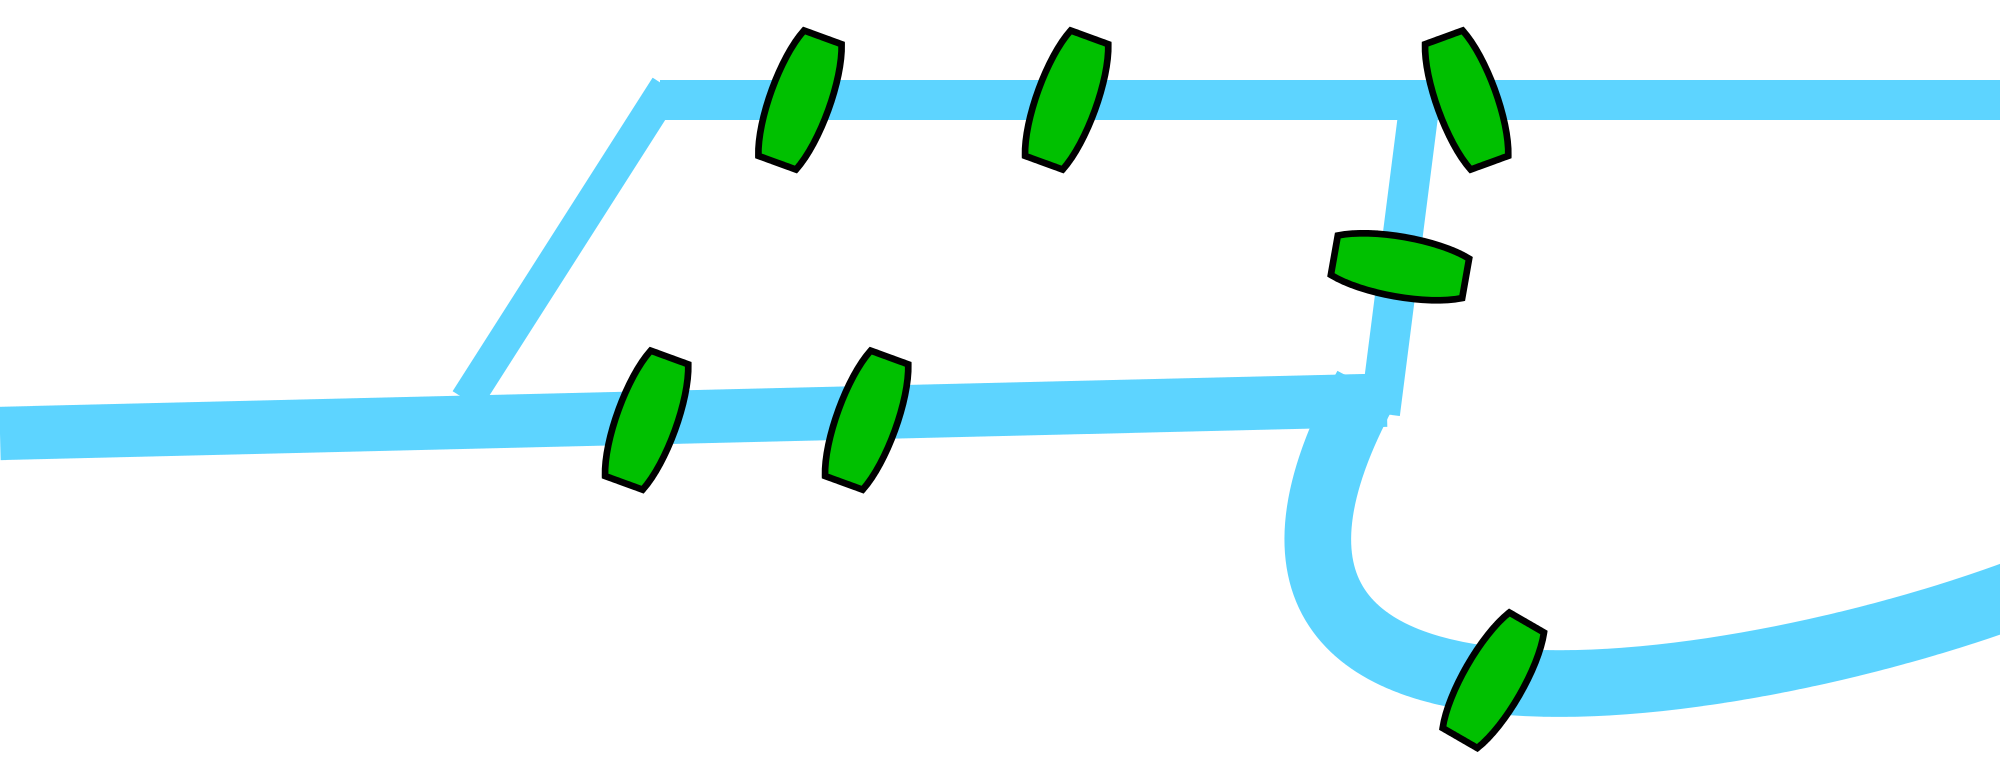
\includegraphics[width=10cm]{bridges.png} 
   \begin{center}
       \caption{\label{fig:my-label}Figure 1.1: Seven Bridges of K\"{o}nigsberg in Prussia}
   \end{center}
\end{center}


\indent This problem is also known as the “Seven Bridges of K\"{o}nigsberg” and is given a different approach by representing the four land masses in a form of a dot, and the bridges in a form of a line. These representations are collectively known as a graph. Graphs are made up of a collection of dots called vertices and lines connecting those dots called edges.\\

\indent A graph on $n$ vertices is said to be graceful if we can label all its vertices with integers from 0 to $n$, such that when an edge is labeled as the absolute difference of the numbers assigned to the vertices joining the edge, the edge will run from 1 to $n-1$.\\

\indent A tree is a connected simple graph without any cycles, or a tree is a connect acyclic graph. A tree on $n$ vertices is said to be graceful if its vertices can be labeled from 0 to $n-1$ such that the edge weights, that is equal to the absolute difference of the adjacent vertices, will run from 1 to $n-1$.\\

\indent In 1967, Gerhard Ringel and Anton Kotzig hypothesized that all trees are graceful. Up to this date,this conjecture has not yet proven, although some researches proved specific classes of trees. This problem lead to the discovery of new families of trees and some graceful labelling algorithms.

\section{Statement of the Problem}
\indent The problem in this study is to find and discover at least one new family of graceful trees in order to support and further strengthen the Ringel-Kotzig conjecture. 

\section{Objectives of the Study}
\indent
The main objective of this study is to discover at least one family of graceful
trees.

\par Specifically, it aims to:

\begin{enumerate}

\item \noindent provide readers sufficient background information about the Graceful Tree Conjecture;

\item \noindent provide a compilation of known families of graceful trees;

\item \noindent identify at least one family of graceful trees which is not yet shown to be graceful; and

\item \noindent find an interlaced graceful valuation of every member of the family of trees identified.

\end{enumerate}

\section{Significance of the Study}

\indent Since the introduction of the Ringel - Kotzig conjecture in 1967, many attempts were made in order to confirm the validity of the said conjecture. However, the conjecture remains unproven until now. No direct proof has been formulated yet but it was suggested that the conjecture can be indirectly proven by assuming that there is a tree that is not graceful. With it being not graceful, it should not be isomorphic to any member of discovered families of graceful trees. Thus, this study is significant in finding and discovering new families of graceful trees in order to support and further strengthen the conjecture.

\section{Scope and Limitations of the Study}

\indent Although most graphs can be gracefully-labeled, this study dealt only with graceful numbering of trees and while there are various graceful labeling of graphs, this study focuses only on the interlaced graceful valuation of trees.

\section{Time and Place of the Study}

\indent This study was conducted at the Mathematics Division, Institute of Mathematical Sciences and Physics, College of Arts and Sciences, University of the Philippines Los Ba\~{n}os, from January 2019 to May 2019.

\newpage
\chapter{REVIEW OF RELATED LITERATURE}
\thispagestyle{empty}

\indent
One of the most well-known unproven conjectures in Graph Theory is the Ringel - Kotzig conjecture. In 1963, Ringel and Kotzig hypothesized that all trees are graceful. Since the introduction of the Ringel–Kotzig conjecture, many attempts were made in order to confirm the validity of the said conjecture. As of now, many families of graceful trees have been found to support the conjecture. Here are some known families of graceful trees.


\begin{enumerate}
	
	\item \noindent {\bfseries Path}\\
	A path (or chain) is a walk with distinct vertices and edges. Shown in the figure below is a gracefully-labeled path on 7 vertices.\\

	\begin{center}
	\resizebox {0.5\textwidth} {0.5\height} {
		
		\begin{tikzpicture}[shorten >=1pt, auto, node distance=3cm,
		node_style/.style={circle,draw=black,fill=white!20!,font=\sffamily},
		edge_style/.style={draw=black}]
		\node[node_style] (n0) at (4,9)  {0};
		\node[node_style] (n6) at (7,9) {6};
		\node[node_style] (n1) at (10,9)  {1};
		\node[node_style] (n5) at (13,9)  {5};
		\node[node_style] (n2) at (16,9) {2};
		\node[node_style] (n4) at (19,9)  {4};
		\node[node_style] (n3) at (22,9)  {3};
		\draw[edge_style]  (n0) edge node{6} (n6);
		\draw[edge_style]  (n6) edge node{5} (n1);
		\draw[edge_style]  (n1) edge node{4} (n5);
		\draw[edge_style]  (n5) edge node{3} (n2);
		\draw[edge_style]  (n2) edge node{2} (n4);
		\draw[edge_style]  (n4) edge node{1} (n3);
		\end{tikzpicture}}
\end{center}
		



	\item \noindent {\bfseries Caterpillars}\\
	A caterpillar is a tree where the removal of its vertices of degree one leaves a path. Shown in the figure below is a gracefully-labeled caterpillar on 14 vertices.\\
	\begin{center}
		\resizebox {0.6\textwidth} {0.5\height} {
			\begin{tikzpicture}[shorten >=1pt, auto, node distance=3cm,
			node_style/.style={circle,draw=black,fill=white!20!,font=\sffamily},
			edge_style/.style={draw=black}]
			\node[node_style] (n12) at (7,11)  {12};
			\node[node_style] (n9) at (13,11) {9};
			\node[node_style] (n5) at (16,11)  {5};
			\node[node_style] (n13) at (3,9)  {13};
			\node[node_style] (n2) at (7,9) {2};
			\node[node_style] (n10) at (10,9)  {10};
			\node[node_style] (n4) at (13,9)  {4};
			\node[node_style] (n8) at (16,9)  {8};
			\node[node_style] (n6) at (19,9) {6};
			\node[node_style] (n0) at (1,7)  {0};
			\node[node_style] (n1) at (4,7)  {1};
			\node[node_style] (n11) at (7,7) {11};
			\node[node_style] (n3) at (10,7)  {3};
			\node[node_style] (n7) at (16,7)  {7};
			\draw[edge_style]  (n0) edge node{13} (n13);
			\draw[edge_style]  (n1) edge node{12} (n13);
			\draw[edge_style]  (n2) edge node{11} (n13);
			\draw[edge_style]  (n2) edge node{9} (n11);
			\draw[edge_style]  (n2) edge node{10} (n12);
			\draw[edge_style]  (n2) edge node{8} (n10);
			\draw[edge_style]  (n3) edge node{7} (n10);
			\draw[edge_style]  (n4) edge node{6} (n10);
			\draw[edge_style]  (n4) edge node{5} (n9);
			\draw[edge_style]  (n4) edge node{4} (n8);
			\draw[edge_style]  (n5) edge node{3} (n8);
			\draw[edge_style]  (n7) edge node{1} (n8);
			\draw[edge_style]  (n8) edge node{2} (n6);
			\end{tikzpicture}}
\end{center}	

	\item \noindent {\bfseries Symmetrical Trees}\\
A symmetrical tree is a rooted tree in which every level contains vertices of the same degree. Shown in the figure below is a gracefully-labeled symmetrical tree on 11 vertices.\\
\begin{center}
	\resizebox {0.3\textwidth} {0.5\height} {
		\begin{tikzpicture}[shorten >=1pt, auto, node distance=3cm,
		node_style/.style={circle,draw=black,fill=white!20!,font=\sffamily},
		edge_style/.style={draw=black}]
		\node[node_style] (n0) at (5,13)  {0};
		\node[node_style] (n10) at (3,11) {10};
		\node[node_style] (n6) at (7,11)  {6};
		\node[node_style] (n1) at (2,9) {1};
		\node[node_style] (n3) at (4,9)  {3};
		\node[node_style] (n8) at (6,9)  {8};
		\node[node_style] (n2) at (8,9)  {2};
		\node[node_style] (n9) at (2,7) {9};
		\node[node_style] (n4) at (4,7)  {4};
		\node[node_style] (n5) at (6,7)  {5};
		\node[node_style] (n7) at (8,7)  {7};
		\draw[edge_style]  (n0) edge node{10} (n10);
		\draw[edge_style]  (n0) edge node{6} (n6);
		\draw[edge_style]  (n10) edge node{9} (n1);
		\draw[edge_style]  (n10) edge node{7} (n3);
		\draw[edge_style]  (n6) edge node{2} (n8);
		\draw[edge_style]  (n6) edge node{4} (n2);
		\draw[edge_style]  (n1) edge node{8} (n9);
		\draw[edge_style]  (n3) edge node{1} (n4);
		\draw[edge_style]  (n8) edge node{3} (n5);
		\draw[edge_style]  (n2) edge node{5} (n7);
		\end{tikzpicture}}
\end{center}	

	\item \noindent {\bfseries Spider Trees}\\
A spider tree is a tree with one vertex of degree at least 3 and all others with degree at most 2. Shown in the figure below is a gracefully-labeled spider tree on 7 vertices.\\
\begin{center}
	\resizebox {0.2\textwidth} {0.4\height} {
		\begin{tikzpicture}[shorten >=1pt, auto, node distance=3cm,
		node_style/.style={circle,draw=black,fill=white!20!,font=\sffamily},
		edge_style/.style={draw=black}]
		\node[node_style] (n5) at (1,13)  {5};
		\node[node_style] (n1) at (9,13) {1};
		\node[node_style] (n0) at (3,11)  {0};
		\node[node_style] (n4) at (7,11) {4};
		\node[node_style] (n6) at (5,9)  {6};
		\node[node_style] (n2) at (5,7)  {2};
		\node[node_style] (n3) at (5,5)  {3};
		\draw[edge_style]  (n5) edge node{5} (n0);
		\draw[edge_style]  (n1) edge node{3} (n4);
		\draw[edge_style]  (n0) edge node{6} (n6);
		\draw[edge_style]  (n4) edge node{2} (n6);
		\draw[edge_style]  (n6) edge node{4} (n2);
		\draw[edge_style]  (n3) edge node{1} (n2);
		\end{tikzpicture}}
\end{center}	

\item \noindent {\bfseries Stars}\\
A star is a special case of caterpillar where the deletion of its end vertices results into a single vertex or a point. Shown in the figure below is a gracefully-labeled star of 5 vertices.\\
\begin{center}
	\resizebox {0.15\textwidth} {0.4\height} {
		\begin{tikzpicture}[shorten >=1pt, auto, node distance=3cm,
		node_style/.style={circle,draw=black,fill=white!20!,font=\sffamily},
		edge_style/.style={draw=black}]
		\node[node_style] (n1) at (3,11)  {1};
		\node[node_style] (n4) at (3,7) {4};
		\node[node_style] (n0) at (5,9)  {0};
		\node[node_style] (n2) at (7,11) {2};
		\node[node_style] (n3) at (7,7)  {3};
		\draw[edge_style]  (n1) edge node{1} (n0);
		\draw[edge_style]  (n0) edge node{4} (n4);
		\draw[edge_style]  (n0) edge node{2} (n2);
		\draw[edge_style]  (n0) edge node{3} (n3);
		\end{tikzpicture}}
\end{center}	


	\item \noindent {\bfseries $M$-stars}\\
A tree with one vertex acting as the root of paths of length $m$ is called an $m$-star. Shown in the figure below is a gracefully-labeled 3-star of 13 vertices.\\
\begin{center}
	\resizebox {0.2\textwidth} {0.4\height} {
		\begin{tikzpicture}[shorten >=1pt, auto, node distance=3cm,
		node_style/.style={circle,draw=black,fill=white!20!,font=\sffamily},
		edge_style/.style={draw=black}]
		\node[node_style] (n0) at (4,13)  {0};
		\node[node_style] (n12) at (1,11) {12};
		\node[node_style] (n4) at (4,11)  {4};
		\node[node_style] (n8) at (7,11) {8};
		\node[node_style] (n1) at (1,9)  {2};
		\node[node_style] (n9) at (4,9)  {9};
		\node[node_style] (n5) at (7,9)  {5};	
		\node[node_style] (n11) at (1,7) {11};
		\node[node_style] (n3) at (4,7)  {3};
		\node[node_style] (n7) at (7,7) {7};
		\node[node_style] (n2) at (1,5)  {2};
		\node[node_style] (n10) at (4,5)  {10};
		\node[node_style] (n6) at (7,5)  {6};
		\draw[edge_style]  (n0) edge node{12} (n12);
		\draw[edge_style]  (n0) edge node{4} (n4);
		\draw[edge_style]  (n0) edge node{8} (n8);
		\draw[edge_style]  (n12) edge node{11} (n1);
		\draw[edge_style]  (n1) edge node{10} (n11);
		\draw[edge_style]  (n11) edge node{9} (n2);
		\draw[edge_style]  (n4) edge node{5} (n9);
		\draw[edge_style]  (n9) edge node{6} (n3);
		\draw[edge_style]  (n3) edge node{7} (n10);
		\draw[edge_style]  (n8) edge node{3} (n5);
		\draw[edge_style]  (n5) edge node{2} (n7);
		\draw[edge_style]  (n7) edge node{1} (n6);
		\end{tikzpicture}}
\end{center}	

	\item \noindent {\bfseries Banana Trees}\\
A banana tree is a graph obtained by joining an end vertex of a star to a single vertex not in the star by an edge. Shown in the figure below is a gracefully-labeled banana tree of 11 vertices.\\
\begin{center}
	\resizebox {0.3\textwidth} {0.5\height} {
		\begin{tikzpicture}[shorten >=1pt, auto, node distance=3cm,
		node_style/.style={circle,draw=black,fill=white!20!,font=\sffamily},
		edge_style/.style={draw=black}]
		\node[node_style] (n1) at (6,11)  {1};
		\node[node_style] (n8) at (3,9) {8};
		\node[node_style] (n7) at (6,9)  {7};
		\node[node_style] (n5) at (9,9) {5};
		\node[node_style] (n0) at (3,7)  {0};
		\node[node_style] (n2) at (6,7)  {2};
		\node[node_style] (n6) at (9,7)  {6};	
		\node[node_style] (n9) at (1,5) {9};
		\node[node_style] (n10) at (5,5)  {10};
		\node[node_style] (n3) at (7,5) {3};
		\node[node_style] (n4) at (11,5)  {4};
		\draw[edge_style]  (n1) edge node{7} (n8);
		\draw[edge_style]  (n1) edge node{6} (n7);
		\draw[edge_style]  (n1) edge node{4} (n5);
		\draw[edge_style]  (n8) edge node{8} (n0);
		\draw[edge_style]  (n7) edge node{5} (n2);
		\draw[edge_style]  (n5) edge node{1} (n6);
		\draw[edge_style]  (n0) edge node{9} (n9);
		\draw[edge_style]  (n0) edge node{10} (n10);
		\draw[edge_style]  (n6) edge node{3} (n3);
		\draw[edge_style]  (n6) edge node{2} (n4);

		\end{tikzpicture}}
\end{center}		

	\item \noindent {\bfseries Firecrackers}\\
A firecracker is a tree consisting of a path $P$ and a collection of stars, where each vertex of $P$ is joined to the central vertex of exactly one star. Shown in the figure below is a gracefully-labeled firecracker of 9 vertices.\\
\begin{center}
	\resizebox {0.3\textwidth} {0.5\height} {
		\begin{tikzpicture}[shorten >=1pt, auto, node distance=3cm,
		node_style/.style={circle,draw=black,fill=white!20!,font=\sffamily},
		edge_style/.style={draw=black}]
		\node[node_style] (n5) at (1,11)  {5};
		\node[node_style] (n6) at (3,11) {6};
		\node[node_style] (n7) at (5,11)  {7};
		\node[node_style] (n3) at (7,11) {3};
		\node[node_style] (n2) at (9,11)  {2};
		\node[node_style] (n0) at (3,9)  {0};
		\node[node_style] (n1) at (8,9)  {1};	
		\node[node_style] (n8) at (3,7) {8};
		\node[node_style] (n4) at (8,7)  {4};
		\draw[edge_style]  (n0) edge node{5} (n5);
		\draw[edge_style]  (n0) edge node{6} (n6);
		\draw[edge_style]  (n0) edge node{7} (n7);
		\draw[edge_style]  (n0) edge node{8} (n8);
		\draw[edge_style]  (n1) edge node{1} (n2);
		\draw[edge_style]  (n1) edge node{2} (n3);
		\draw[edge_style]  (n1) edge node{3} (n4);
		\draw[edge_style]  (n4) edge node{4} (n8);		
		\end{tikzpicture}}
\end{center}		


	\item \noindent {\bfseries Lobster Trees}\\
A lobster tree is a tree such that the removal of its leaves results into a caterpillar. Shown in the figure below is a gracefully-labeled lobster tree of 26 vertices.\\
\begin{center}
	\resizebox {0.9\textwidth} {0.4\height} {
		\begin{tikzpicture}[shorten >=1pt, auto, node distance=3cm,
		node_style/.style={circle,draw=black,fill=white!20!,font=\sffamily},
		edge_style/.style={draw=black}]
		\node[node_style] (n25) at (27,13)  {25};
		\node[node_style] (n12) at (9,11) {12};
		\node[node_style] (n8) at (21,11)  {8};
		\node[node_style] (n4) at (27,11) {4};
		\node[node_style] (n0) at (33,11)  {0};
		\node[node_style] (n13) at (3,9)  {13};
		\node[node_style] (n17) at (9,9)  {17};	
		\node[node_style] (n21) at (15,9) {21};
		\node[node_style] (n16) at (19,9)  {16};
		\node[node_style] (n15) at (21,9)  {15};
		\node[node_style] (n14) at (23,9) {14};
		\node[node_style] (n20) at (25,9)  {20};
		\node[node_style] (n19) at (27,9) {19};
		\node[node_style] (n18) at (29,9)  {18};
		\node[node_style] (n24) at (31,9)  {24};
		\node[node_style] (n23) at (33,9)  {23};	
		\node[node_style] (n22) at (35,9) {22};
		\node[node_style] (n11) at (1,7)  {11};
		\node[node_style] (n10) at (3,7) {10};
		\node[node_style] (n9) at (5,7)  {9};
		\node[node_style] (n7) at (7,7) {7};
		\node[node_style] (n6) at (9,7)  {6};
		\node[node_style] (n5) at (11,7)  {5};
		\node[node_style] (n3) at (13,7)  {3};	
		\node[node_style] (n2) at (15,7) {2};
		\node[node_style] (n1) at (17,7)  {1};
		\draw[edge_style]  (n25) edge node{13} (n12);
		\draw[edge_style]  (n25) edge node{17} (n8);
		\draw[edge_style]  (n25) edge node{21} (n4);
		\draw[edge_style]  (n25) edge node{25} (n0);
		\draw[edge_style]  (n12) edge node{1} (n13);
		\draw[edge_style]  (n12) edge node{5} (n17);
		\draw[edge_style]  (n12) edge node{9} (n21);
		\draw[edge_style]  (n8) edge node{8} (n16);
		\draw[edge_style]  (n8) edge node{7} (n15);
		\draw[edge_style]  (n8) edge node{6} (n14);
		\draw[edge_style]  (n4) edge node{16} (n20);
		\draw[edge_style]  (n4) edge node{15} (n19);
		\draw[edge_style]  (n4) edge node{14} (n18);
		\draw[edge_style]  (n0) edge node{24} (n24);
		\draw[edge_style]  (n0) edge node{23} (n23);
		\draw[edge_style]  (n0) edge node{22} (n22);
		\draw[edge_style]  (n13) edge node{2} (n11);
		\draw[edge_style]  (n13) edge node{3} (n10);
		\draw[edge_style]  (n13) edge node{4} (n9);
		\draw[edge_style]  (n17) edge node{10} (n7);
		\draw[edge_style]  (n17) edge node{11} (n6);
		\draw[edge_style]  (n17) edge node{12} (n5);
		\draw[edge_style]  (n21) edge node{18} (n3);
		\draw[edge_style]  (n21) edge node{19} (n2);
		\draw[edge_style]  (n21) edge node{20} (n1);
		\end{tikzpicture}}
\end{center}		


	\item \noindent {\bfseries Regular Bamboo Trees}\\
A regular bamboo tree consists of legs with equal lengths attached to a
single vertex. The leaves of this tree are leaves of stars with the same size. Shown in the figure below is a gracefully-labeled regular bamboo tree of 43 vertices.\\
\begin{center}
	\resizebox {0.9\textwidth} {0.4\height} {
		\begin{tikzpicture}[shorten >=1pt, auto, node distance=3cm,
		node_style/.style={circle,draw=black,fill=white!20!,font=\sffamily},
		edge_style/.style={draw=black}]
		\node[node_style] (n0) at (18,13)  {0};
		\node[node_style] (n42) at (33,11) {42};
		\node[node_style] (n35) at (27,11)  {35};
		\node[node_style] (n28) at (21,11) {28};
		\node[node_style] (n21) at (15,11)  {21};
		\node[node_style] (n14) at (9,11)  {14};
		\node[node_style] (n7) at (3,11)  {7};	
		\node[node_style] (n1) at (33,9) {1};
		\node[node_style] (n8) at (27,9)  {8};
		\node[node_style] (n15) at (21,9)  {15};
		\node[node_style] (n22) at (15,9)  {22};
		\node[node_style] (n29) at (9,9) {29};
		\node[node_style] (n36) at (3,9)  {36};
		\node[node_style] (n41) at (33,7)  {41};
		\node[node_style] (n34) at (27,7)  {34};	
		\node[node_style] (n27) at (21,7) {27};
		\node[node_style] (n20) at (15,7)  {20};
		\node[node_style] (n13) at (9,7) {13};
		\node[node_style] (n6) at (3,7)  {6};
		\node[node_style] (n2) at (33,5) {2};
		\node[node_style] (n9) at (27,5)  {9};
		\node[node_style] (n16) at (21,5)  {16};
		\node[node_style] (n23) at (15,5)  {23};	
		\node[node_style] (n30) at (9,5) {30};
		\node[node_style] (n37) at (3,5)  {37};
		\node[node_style] (n40) at (35,3)  {40};
		\node[node_style] (n39) at (33,3) {39};
		\node[node_style] (n38) at (31,3)  {38};
		\node[node_style] (n33) at (29,3) {33};
		\node[node_style] (n32) at (27,3)  {32};
		\node[node_style] (n31) at (25,3)  {31};
		\node[node_style] (n26) at (23,3)  {26};	
		\node[node_style] (n25) at (21,3) {25};
		\node[node_style] (n24) at (19,3)  {24};
		\node[node_style] (n19) at (17,3) {19};
		\node[node_style] (n18) at (15,3)  {18};
		\node[node_style] (n17) at (13,3) {17};
		\node[node_style] (n12) at (11,3)  {12};
		\node[node_style] (n11) at (9,3)  {11};
		\node[node_style] (n10) at (7,3)  {10};	
		\node[node_style] (n5) at (5,3) {5};
		\node[node_style] (n4) at (3,3)  {4};
		\node[node_style] (n3) at (1,3)  {3};
		\draw[edge_style]  (n0) edge node{42} (n42);
		\draw[edge_style]  (n0) edge node{35} (n35);
		\draw[edge_style]  (n0) edge node{28} (n28);
		\draw[edge_style]  (n0) edge node{21} (n21); 
		\draw[edge_style]  (n0) edge node{14} (n14);
		\draw[edge_style]  (n0) edge node{7} (n7);
		\draw[edge_style]  (n42) edge node{41} (n1);
		\draw[edge_style]  (n35) edge node{27} (n8);
		\draw[edge_style]  (n28) edge node{13} (n15);
		\draw[edge_style]  (n21) edge node{1} (n22);
		\draw[edge_style]  (n14) edge node{15} (n29);
		\draw[edge_style]  (n7) edge node{29} (n36);
		\draw[edge_style]  (n1) edge node{40} (n41);
		\draw[edge_style]  (n8) edge node{26} (n34);
		\draw[edge_style]  (n15) edge node{12} (n27);
		\draw[edge_style]  (n22) edge node{2} (n20);
		\draw[edge_style]  (n29) edge node{16} (n13);
		\draw[edge_style]  (n36) edge node{30} (n6);
		\draw[edge_style]  (n41) edge node{39} (n2);
		\draw[edge_style]  (n34) edge node{25} (n9);
		\draw[edge_style]  (n27) edge node{11} (n16);
		\draw[edge_style]  (n20) edge node{3} (n23);
		\draw[edge_style]  (n13) edge node{17} (n30);
		\draw[edge_style]  (n6) edge node{31} (n37);
		\draw[edge_style]  (n2) edge node{38} (n40);
		\draw[edge_style]  (n2) edge node{37} (n39);		 \draw[edge_style]  (n2) edge node{36} (n38);		\draw[edge_style]  (n9) edge node{24} (n33);	  	
		\draw[edge_style]  (n9) edge node{23} (n32);	   
		\draw[edge_style]  (n9) edge node{22} (n31);		
		\draw[edge_style]  (n16) edge node{10} (n26);		\draw[edge_style]  (n16) edge node{9} (n25);		\draw[edge_style]  (n16) edge node{8} (n24);		\draw[edge_style]  (n23) edge node{4} (n19);		\draw[edge_style]  (n23) edge node{5} (n18);		\draw[edge_style]  (n23) edge node{6} (n17);		\draw[edge_style]  (n30) edge node{18} (n12);		\draw[edge_style]  (n30) edge node{19} (n11);		\draw[edge_style]  (n30) edge node{20} (n10);		\draw[edge_style]  (n37) edge node{32} (n5);		\draw[edge_style]  (n37) edge node{33} (n4);		\draw[edge_style]  (n37) edge node{34} (n3);
		\end{tikzpicture}}
\end{center}		

%11
\item {\bfseries Olive Trees}\\
    An Olive tree is formed by attaching paths of consecutive lengths in a single vertex. Shown below is an example 
	\\
	\begin{center}
	\resizebox {0.3\textwidth} {0.7\height} {
		\begin{tikzpicture}[shorten >=2pt, auto, node distance=1cm,
		node_style/.style={circle,draw=black,fill=white!0!,font=\sffamily},
		edge_style/.style={draw=black}]
		
		\node[node_style] (n15) at (3,3)  {15};
		\node[node_style] (n12) at (5,2)  {12};
		\node[node_style] (n5) at (4.5,0.5)  {5};
		\node[node_style] (n9) at (4.5,-1)  {9};
		\node[node_style] (n6) at (3.5,0)  {6};
		\node[node_style] (n8) at (3.5,-1.5)  {8};
		\node[node_style] (n7) at (3.5,-3)  {7};
		\node[node_style] (n10) at (1,0)  {10};
		\node[node_style] (n4) at (1,-1.5)  {4};
		\node[node_style] (n11) at (1,-3)  {11};
		\node[node_style] (n3) at (1,-4.5)  {3};
		\node[node_style] (n0) at (-0.5,1)  {0};
		\node[node_style] (n14) at (-0.5,-1.5)  {14};
		\node[node_style] (n1) at (-0.5,-3)  {1};
	    \node[node_style] (n13) at (-0.5,-4.5)  {13};
		\node[node_style] (n2) at (-0.5,-6)  {2};
		
		\draw[edge_style]  (n15) edge node{3} (n12);
    	\draw[edge_style]  (n15) edge node{10} (n5);
    	\draw[edge_style]  (n5) edge node{4} (n9);
    	\draw[edge_style]  (n15) edge node{9} (n6);
    	\draw[edge_style]  (n6) edge node{2} (n8);
    	\draw[edge_style]  (n8) edge node{1} (n7);
    	\draw[edge_style]  (n15) edge node{5} (n10);
    	\draw[edge_style]  (n10) edge node{6} (n4);
    	\draw[edge_style]  (n4) edge node{7} (n11);
    	\draw[edge_style]  (n11) edge node{8} (n3);
    	\draw[edge_style]  (n15) edge node{15} (n0);
    	\draw[edge_style]  (n0) edge node{14} (n14);
    	\draw[edge_style]  (n14) edge node{13} (n1);
    	\draw[edge_style]  (n1) edge node{12} (n13);
    	\draw[edge_style]  (n13) edge node{11} (n2);
    
		\end{tikzpicture}}
		\begin{center}
		    Figure "insert number": A graceful olive tree
		\end{center}
		
\end{center}

    Dr. Jean Loyola discovered three new families of graceful trees.
%12	
\item {\bfseries $J_n$ Trees}\\
    $J_n$ trees are constructed by planting an end vertex of a path of length $i$, for $i=0,1,2,...,n-1$, in a parent path $v_0 v_1 v_2...v_{n-1}$ with a length of $n-1$. Shown below is an example of a graceful $J_4$ tree.
    \\
\newpage
	\begin{center}
	\resizebox {0.3\textwidth} {0.7\height} {
		\begin{tikzpicture}[shorten >=2pt, auto, node distance=1cm,
		node_style/.style={circle,draw=black,fill=white!0!,font=\sffamily},
		edge_style/.style={draw=black}]
		
		\node[node_style] (n0) at (0,0)  {0};
		\node[node_style] (n9) at (2,0)  {9};
		\node[node_style] (n2) at (4,0)  {2};
		\node[node_style] (n6) at (6,0)  {6};
		\node[node_style] (n1) at (2,2)  {1};
		\node[node_style] (n8) at (4,2)  {8};
		\node[node_style] (n3) at (4,4)  {3};
		\node[node_style] (n5) at (6,2)  {5};
		\node[node_style] (n7) at (6,4)  {7};
		\node[node_style] (n4) at (6,6)  {4};
		
		
		\draw[edge_style]  (n0) edge node{9} (n9);
    	\draw[edge_style]  (n9) edge node{7} (n2);
    	\draw[edge_style]  (n2) edge node{4} (n6);
    	\draw[edge_style]  (n9) edge node{8} (n1);
    	\draw[edge_style]  (n2) edge node{6} (n8);
    	\draw[edge_style]  (n8) edge node{5} (n3);
    	\draw[edge_style]  (n6) edge node{1} (n5);
    	\draw[edge_style]  (n5) edge node{2} (n7);
    	\draw[edge_style]  (n7) edge node{3} (n4);
		\end{tikzpicture}}
		
	
		
\end{center}
%13	
\item {\bfseries $J_{n,m}$ Trees}\\
    A $J_{n,m}$ tree is formed by taking $m$ copies of the $J_n$ tree and making the classification $v_{0,i}=v_{0,j}$ for all $0 {\geq} i$, $j {\geq} m$, provided that $m,n {\geq} 2$.Shown below is an example of a graceful $J_{3,3}$ tree.
	\\
	\begin{center}
	\resizebox {0.5\textwidth} {0.7\height} {
		\begin{tikzpicture}[shorten >=2pt, auto, node distance=1cm,
		node_style/.style={circle,draw=black,fill=white!0!,font=\sffamily},
		edge_style/.style={draw=black}]
		
		\node[node_style] (n0) at (3,0)  {0};
		\node[node_style] (n15) at (5,1)  {15};
		\node[node_style] (n10) at (1,1)  {10};
		\node[node_style] (n5) at (3,-2)  {5};
		\node[node_style] (n12) at (3,-4)  {12};
		\node[node_style] (n11) at (1,-2)  {11};
		\node[node_style] (n4) at (1,-4)  {4};
		\node[node_style] (n13) at (-1,-4)  {5};
		\node[node_style] (n7) at (-1,2)  {7};
		\node[node_style] (n6) at (3,2)  {6};
		\node[node_style] (n1) at (7,0)  {1};
		\node[node_style] (n2) at (7,2)  {2};
		\node[node_style] (n14) at (9,1)  {14};
		\node[node_style] (n3) at (11,0)  {3};
		\node[node_style] (n9) at (1,3)  {9};
		\node[node_style] (n8) at (3,4)  {8};
		
		\draw[edge_style]  (n0) edge node{10} (n10);
    	\draw[edge_style]  (n10) edge node{3} (n7);
    	\draw[edge_style]  (n7) edge node{2} (n9);
    	\draw[edge_style]  (n9) edge node{1} (n8);
    	\draw[edge_style]  (n10) edge node{4} (n6);
    	\draw[edge_style]  (n0) edge node{15} (n15);
    	\draw[edge_style]  (n15) edge node{14} (n1);
    	\draw[edge_style]  (n15) edge node{13} (n2);
    	\draw[edge_style]  (n2) edge node{12} (n14);
        \draw[edge_style]  (n14) edge node{11} (n3);
        \draw[edge_style]  (n0) edge node{5} (n5);
    	\draw[edge_style]  (n5) edge node{6} (n11);
    	\draw[edge_style]  (n5) edge node{7} (n12);
    	\draw[edge_style]  (n12) edge node{8} (n4);
        \draw[edge_style]  (n13) edge node{9} (n4);
    
		\end{tikzpicture}}
		
		
		
\end{center}

%14
\item {\bfseries $J_n$ + $J_{n+1}$ Trees}\\

    \indent 
    A  $J_n$ + $J_{n+1}$ tree is formed considering  $J_n$ and $J_{n+1}$ and making the identification
   
    $v_{i,n}=v_{i+n,n+1}$ for all $1\leq i\leq n-1$.Shown below is an example of a graceful $J_2$ + $J_3$ tree.
	\\
	\begin{center}
	\resizebox {0.3\textwidth} {0.7\height} {
		\begin{tikzpicture}[shorten >=2pt, auto, node distance=1cm,
		node_style/.style={circle,draw=black,fill=white!0!,font=\sffamily},
		edge_style/.style={draw=black}]
		
		\node[node_style] (n5) at (0,0)  {5};
		\node[node_style] (n2) at (2,0)  {2};
		\node[node_style] (n4) at (4,0)  {4};
		\node[node_style] (n3) at (6,0)  {3};
		\node[node_style] (n6) at (2,2)  {6};
		\node[node_style] (n0) at (2,4)  {0};
		\node[node_style] (n1) at (4,2)  {1};
	
		
		\draw[edge_style]  (n5) edge node{3} (n2);
    	\draw[edge_style]  (n2) edge node{2} (n4);
    	\draw[edge_style]  (n4) edge node{1} (n3);
    	\draw[edge_style]  (n2) edge node{4} (n6);
    	\draw[edge_style]  (n0) edge node{6} (n6);
    	\draw[edge_style]  (n6) edge node{5} (n1);
    
    
		\end{tikzpicture}}
		
		
\end{center}

%15
\newpage
Castilan and Zarraga discover three new familes of graceful trees namely, $\overline{P}_{(0,1)_n}(f)$,  $\overline{P}_{(0,2)_n}(f)$, and  $\overline{P}_{(0,3)_n}(f)$
\item {\bfseries $\overline{P}_{(0,1)_n}(f)$ Trees}\\
    % NEEDS DEFINITION
    Let $f(i)=k$ if $n=2k-1$ or $n=2k$. Let  $\overline{P}_{(0,1)_n}(f)=v_0 v_1 v_2\dots v_n$ be a path of length $n$ where $n$ is an even integer. Let $\overline{P}_{(0,1)_n}(f)$ be the tree obtained by planting an end vertex of a path $\overline{P}_i$ of length $f(i)$ to each $v_i$ for $i=1,2,\dots,n$. Shown below is an example of a graceful $\overline{P}_{(0,1)_4}(f)$ tree.
	\\
	\begin{center}
	\resizebox {0.4\textwidth} {0.7\height} {
		\begin{tikzpicture}[shorten >=2pt, auto, node distance=1cm,
		node_style/.style={circle,draw=black,fill=white!0!,font=\sffamily},
		edge_style/.style={draw=black}]
		
		\node[node_style] (n0) at (0,0)  {0};
		\node[node_style] (n10) at (2,0)  {10};
		\node[node_style] (n1) at (2,2)  {1};
		\node[node_style] (n2) at (4,0)  {2};
		\node[node_style] (n9) at (4,2)  {9};
		\node[node_style] (n8) at (6,0)  {8};
		\node[node_style] (n3) at (6,2)  {3};
	    \node[node_style] (n7) at (6,4)  {7};
		\node[node_style] (n5) at (8,0)  {5};
		\node[node_style] (n6) at (8,2)  {6};
		\node[node_style] (n4) at (8,4)  {4};
		
		\draw[edge_style]  (n0) edge node{10} (n10);
    	\draw[edge_style]  (n10) edge node{9} (n1);
    	\draw[edge_style]  (n10) edge node{8} (n2);
    	\draw[edge_style]  (n2) edge node{7} (n9);
    	\draw[edge_style]  (n2) edge node{6} (n8);
    	\draw[edge_style]  (n8) edge node{3} (n5);
        \draw[edge_style]  (n8) edge node{5} (n3);
    	\draw[edge_style]  (n3) edge node{4} (n7);
    	\draw[edge_style]  (n5) edge node{1} (n6);
    	\draw[edge_style]  (n6) edge node{2} (n4);
    
		\end{tikzpicture}}

\end{center}

%16 
\item {\bfseries $\overline{P}_{(0,2)_n}(f)$ Trees}\\

    Let $f(i)=k+1$ if $n=2k-1$ or $n=2k$, $k\geq1$. Let $\overline{P}_{(0,2)_n}(f)=v_0 v_1 v_2\dots v_n$ be a path of length $n$ where $n$ is an even integer. Let $\overline{P}_{(0,2)_n}(f)$ be the tree obtained by planting an end vertex of a path $\overline{P}_i$ of length $f(i)$ to each $v_i$ for $i=1,2,\dots,n$. Shown below is an example of a graceful $\overline{P}_{(0,2)_4}(f)$ tree.
	\\
	\begin{center}
	\resizebox {0.4\textwidth} {0.7\height} {
		\begin{tikzpicture}[shorten >=2pt, auto, node distance=1cm,
		node_style/.style={circle,draw=black,fill=white!0!,font=\sffamily},
		edge_style/.style={draw=black}]
		
		\node[node_style] (n0) at (0,0)  {0};
		\node[node_style] (n14) at (2,0)  {14};
		\node[node_style] (n1) at (2,2)  {1};
		\node[node_style] (n13) at (2,4)  {13};
		\node[node_style] (n3) at (4,0)  {3};
		\node[node_style] (n12) at (4,2)  {12};
		\node[node_style] (n2) at (4,4)  {2};
	    \node[node_style] (n11) at (6,0)  {11};
		\node[node_style] (n4) at (6,2)  {4};
		\node[node_style] (n10) at (6,4)  {10};
		\node[node_style] (n5) at (6,6)  {5};
		\node[node_style] (n7) at (8,0)  {7};
		\node[node_style] (n8) at (8,2)  {8};
		\node[node_style] (n6) at (8,4)  {6};
		\node[node_style] (n9) at (8,6)  {9};
		
		
		\draw[edge_style]  (n0) edge node{14} (n14);
    	\draw[edge_style]  (n14) edge node{13} (n1);
    	\draw[edge_style]  (n1) edge node{12} (n13);
    	\draw[edge_style]  (n14) edge node{11} (n3);
    	\draw[edge_style]  (n3) edge node{9} (n12);
    	\draw[edge_style]  (n12) edge node{10} (n2);
        \draw[edge_style]  (n3) edge node{8} (n11);
    	\draw[edge_style]  (n11) edge node{7} (n4);
    	\draw[edge_style]  (n4) edge node{6} (n10);
    	\draw[edge_style]  (n10) edge node{5} (n5);
    	\draw[edge_style]  (n11) edge node{3} (n7);
    	\draw[edge_style]  (n7) edge node{1} (n8);
    	\draw[edge_style]  (n8) edge node{2} (n6);
    	\draw[edge_style]  (n6) edge node{3} (n9);
    
		\end{tikzpicture}}

\end{center}

%17 
\item {\bfseries $\overline{P}_{(0,3)_n}$ $(f)$ Trees}\\

     Let $f(i)=k+2$ if $n=2k-1$ or $n=2k$, $k\geq1$. Let $\overline{P}_{(0,3)_n}(f)=v_0 v_1 v_2\dots v_n$ be a path of length $n$ where $n$ is an even integer. Let $\overline{P}_{(0,3)_n}(f)$ be the tree obtained by planting an end vertex of a path $\overline{P}_i$ of length $f(i)$ to each $v_i$ for $i=1,2,\dots,n$.Shown below is an example of a graceful $\overline{P}_{(0,3)_4}(f)$ tree.
	\\
	\begin{center}
	\resizebox {0.4\textwidth} {0.7\height} {
		\begin{tikzpicture}[shorten >=2pt, auto, node distance=1cm,
		node_style/.style={circle,draw=black,fill=white!0!,font=\sffamily},
		edge_style/.style={draw=black}]
		
		\node[node_style] (n0) at (0,0)  {0};
		\node[node_style] (n18) at (2,0)  {18};
		\node[node_style] (n1) at (2,2)  {1};
		\node[node_style] (n17) at (2,4)  {17};
		\node[node_style] (n2) at (2,6)  {2};
		\node[node_style] (n4) at (4,0)  {4};
		\node[node_style] (n15) at (4,2)  {15};
	    \node[node_style] (n3) at (4,4)  {3};
		\node[node_style] (n16) at (4,6)  {16};
		\node[node_style] (n14) at (6,0)  {14};
		\node[node_style] (n5) at (6,2)  {5};
		\node[node_style] (n13) at (6,4)  {13};
		\node[node_style] (n6) at (6,6)  {6};
		\node[node_style] (n12) at (6,8)  {12};
		\node[node_style] (n9) at (8,0)  {9};
		\node[node_style] (n10) at (8,2)  {10};
		\node[node_style] (n8) at (8,4)  {8};
		\node[node_style] (n11) at (8,6)  {11};
		\node[node_style] (n7) at (8,8)  {7};
		
		
		\draw[edge_style]  (n0) edge node{18} (n18);
    	\draw[edge_style]  (n18) edge node{17} (n1);
    	\draw[edge_style]  (n1) edge node{16} (n17);
    	\draw[edge_style]  (n17) edge node{15} (n2);
    	\draw[edge_style]  (n18) edge node{14} (n4);
    	\draw[edge_style]  (n4) edge node{11} (n15);
        \draw[edge_style]  (n15) edge node{12} (n3);
    	\draw[edge_style]  (n3) edge node{13} (n16);
    	\draw[edge_style]  (n4) edge node{10} (n14);
    	\draw[edge_style]  (n14) edge node{9} (n5);
    	\draw[edge_style]  (n5) edge node{8} (n13);
    	\draw[edge_style]  (n13) edge node{7} (n6);
    	\draw[edge_style]  (n6) edge node{6} (n12);
    	\draw[edge_style]  (n14) edge node{5} (n9);
    	\draw[edge_style]  (n9) edge node{1} (n10);
    	\draw[edge_style]  (n10) edge node{2} (n8);
    	\draw[edge_style]  (n8) edge node{3} (n11);
    	\draw[edge_style]  (n11) edge node{4} (n7);
    
		\end{tikzpicture}}
\end{center}

%18 

Manalo and Rosales generalized the three graceful trees found by Castilan and Zarraga and named the tree $P_{0,m_n} (f)$.
\item {\bfseries $P_{0,m_n}$ $(f)$ Trees}\\

    Let $f(i)=k+m-1$ if $i=2k-1$ or $i=2k$ where $k,m {\geq} 1$. Let $P_{0,m_n}$ $(f)$ tree be the tree obtained by considering a path $P_n = v_0 v_1 v_2...v_n$ of length $f(i)$ to each $v_i$ for $i=1,2,...,n$. 
	\\

%19 
Adaya and Crehencia discovered that all $P_{2n}(f)$ trees are graceful.
\item {\bfseries $P_{2n}(f)$ Trees}\\
    Let $f(n)=$
\begin{cases}
    0, \text{if $n$ is even}\\
    3, \text{if $n=4k-3$, $k \in \mathbb{N}$}\\
    5, \text{if $n=4k-1$, $k \in \mathbb{N}$}.
    
\end{cases}
\\
Let $P_{2n}(f)$ be the tree obtained by considering a path $P_{2n}=v_0 v_1 v_2\dots v_{2n}$ on $2n+1$ vertices and planting to $v_i$ an end vertex of the path $P_i$ of length $f(i)$ for $i=0,1,2,\dots,2n$.Shown below is an example of a graceful $P_8 (f)$ tree.
\newpage
	\begin{center}
	\resizebox {0.7\textwidth} {0.7\height} {
		\begin{tikzpicture}[shorten >=2pt, auto, node distance=1cm,
		node_style/.style={circle,draw=black,fill=white!0!,font=\sffamily},
		edge_style/.style={draw=black}]
		
		\node[node_style] (n0) at (0,0)  {0};
		\node[node_style] (n24) at (2,0)  {24};
		\node[node_style] (n2) at (2,2)  {2};
		\node[node_style] (n23) at (2,4)  {23};
		\node[node_style] (n3) at (2,6)  {3};
		\node[node_style] (n1) at (4,0)  {1};
		\node[node_style] (n20) at (6,0)  {20};
	    \node[node_style] (n6) at (6,2)  {6};
		\node[node_style] (n21) at (6,4)  {21};
		\node[node_style] (n5) at (6,6)  {5};
		\node[node_style] (n22) at (6,8)  {22};
		\node[node_style] (n4) at (6,10)  {4};
		\node[node_style] (n7) at (8,0)  {7};
		\node[node_style] (n19) at (10,0)  {19};
		\node[node_style] (n9) at (10,2)  {9};
		\node[node_style] (n18) at (10,4)  {18};
		\node[node_style] (n10) at (10,6)  {10};
		\node[node_style] (n8) at (12,0)  {8};
		\node[node_style] (n15) at (14,0)  {15};
		\node[node_style] (n13) at (14,2)  {13};
		\node[node_style] (n16) at (14,4)  {16};
		\node[node_style] (n12) at (14,6)  {12};
		\node[node_style] (n17) at (14,8)  {17};
		\node[node_style] (n11) at (14,10)  {11};
		\node[node_style] (n14) at (16,0)  {14};		
		
		\draw[edge_style]  (n0) edge node{24} (n24);
    	\draw[edge_style]  (n24) edge node{22} (n2);
    	\draw[edge_style]  (n2) edge node{21} (n23);
    	\draw[edge_style]  (n23) edge node{20} (n3);
    	\draw[edge_style]  (n24) edge node{23} (n1);
    	\draw[edge_style]  (n1) edge node{19} (n20);
        \draw[edge_style]  (n20) edge node{14} (n6);
    	\draw[edge_style]  (n6) edge node{15} (n21);
    	\draw[edge_style]  (n21) edge node{16} (n5);
    	\draw[edge_style]  (n5) edge node{17} (n22);
    	\draw[edge_style]  (n22) edge node{17} (n4);
    	\draw[edge_style]  (n20) edge node{13} (n7);
    	\draw[edge_style]  (n7) edge node{12} (n19);
    	\draw[edge_style]  (n19) edge node{10} (n9);
    	\draw[edge_style]  (n9) edge node{9} (n18);
    	\draw[edge_style]  (n18) edge node{8} (n10);
    	\draw[edge_style]  (n19) edge node{11} (n8);
    	\draw[edge_style]  (n8) edge node{7} (n15);
    	\draw[edge_style]  (n15) edge node{2} (n13);
    	\draw[edge_style]  (n13) edge node{3} (n16);
    	\draw[edge_style]  (n16) edge node{4} (n12);
    	\draw[edge_style]  (n12) edge node{5} (n17);
    	\draw[edge_style]  (n17) edge node{5} (n11);
    	\draw[edge_style]  (n15) edge node{1} (n14);
    	
		\end{tikzpicture}}

\end{center}

%20
Gonzales and Navarro found four new families of graceful trees namely, $M_n$, $Z_n$, $Z_n + Z_{n+1}$, and $O_n (1,3)$.
\item {\bfseries $M_n$ Trees}\\
    For $n\geq2$, let $M_n$ be the tree formed by considering a path $P_{2n+a}=v_0 v_1 v_2\dots v_2n$ on $n+1$ vertices and planting to $v_{2i-1}$ an end vertex of the path $P_i$ of length $i$, for $1=0,1,2,\dots,n$. Shown below is an example of graceful $M_6$ tree.
	\\
	\begin{center}
	\resizebox {0.5\textwidth} {0.7\height} {
		\begin{tikzpicture}[shorten >=2pt, auto, node distance=1cm,
		node_style/.style={circle,draw=black,fill=white!0!,font=\sffamily},
		edge_style/.style={draw=black}]
		
		\node[node_style] (n0) at (0,0)  {0};
		\node[node_style] (n12) at (2,0)  {12};
		\node[node_style] (n2) at (2,2)  {2};
		\node[node_style] (n1) at (4,0)  {1};
		\node[node_style] (n10) at (6,0)  {10};
		\node[node_style] (n3) at (6,2)  {3};
		\node[node_style] (n11) at (6,4)  {11};
	    \node[node_style] (n4) at (8,0)  {4};
		\node[node_style] (n9) at (10,0)  {9};
		\node[node_style] (n6) at (10,2)  {6};
		\node[node_style] (n8) at (10,4)  {8};
		\node[node_style] (n7) at (10,6)  {7};
		\node[node_style] (n5) at (12,0)  {5};
		
		\draw[edge_style]  (n0) edge node{12} (n12);
    	\draw[edge_style]  (n12) edge node{10} (n2);
    	\draw[edge_style]  (n12) edge node{11} (n1);
    	\draw[edge_style]  (n1) edge node{9} (n10);
    	\draw[edge_style]  (n10) edge node{7} (n3);
    	\draw[edge_style]  (n3) edge node{8} (n11);
        \draw[edge_style]  (n10) edge node{6} (n4);
    	\draw[edge_style]  (n4) edge node{5} (n9);
    	\draw[edge_style]  (n9) edge node{3} (n6);
    	\draw[edge_style]  (n6) edge node{2} (n8);
    	\draw[edge_style]  (n8) edge node{1} (n7);
    	\draw[edge_style]  (n9) edge node{4} (n5);
    
		\end{tikzpicture}}
\end{center}
\item {\bfseries $Z_n$ Trees}
\\
For $n \geq 2$, let $Z_n$ be the tree formed by considering a path $P_{n+1} = v_0 v_1 v_2...v_n$
on n + 1 vertices and planting an end vertex of a path $P_1$ of length 1 to $v_1$ and
$v_2$, and end vertex of $Y_{(\dfrac{1}{2})(i+3)}$ to vi
if i is odd and $Y_{(\dfrac{1}{2})(i+2)}$ to $v_i$
if i is even for
i = 3, 4, 5, ..., n where $Y_{k+2}$ is the caterpillar on k + 2 vertices which has a path
on k vertices with two legs on one of its end vertices.

\begin{center}
	\resizebox {0.6\textwidth} {0.7\height} {
		\begin{tikzpicture}[shorten >=2pt, auto, node distance=1cm,
		node_style/.style={circle,draw=black,fill=white!0!,font=\sffamily},
		edge_style/.style={draw=black}]
		
		\node[node_style] (n0) at (0,0)  {0};
		\node[node_style] (n18) at (2,0)  {18};
		\node[node_style] (n2) at (4,0)  {2};
		\node[node_style] (n16) at (6,0)  {16};
		\node[node_style] (n5) at (8,0) {5};
		\node[node_style] (n13) at (10,0)  {13};
		\node[node_style] (n9) at (12,0)  {9};
		\node[node_style] (n1) at (2,2)  {1};
		\node[node_style] (n17) at (4,2)  {17};
		\node[node_style] (n3) at (5,2)  {3};
		\node[node_style] (n4) at (6.5,2)  {4};
		\node[node_style] (n15) at (7.5,2)  {15};
		\node[node_style] (n14) at (9,2)  {14};
		\node[node_style] (n6) at (10,2)  {6};
		\node[node_style] (n10) at (12,2)  {10};
		\node[node_style] (n12) at (9.3,4)  {12};
		\node[node_style] (n11) at (10.5,4)  {11};
		\node[node_style] (n7) at (11.5,4)  {7};
		\node[node_style] (n8) at (14,4)  {8};
	
	    \draw[edge_style] (n0) edge node{18} (n18);
	    \draw[edge_style] (n18) edge node{17} (n1);
	    \draw[edge_style] (n18) edge node{16} (n2);
	    \draw[edge_style] (n2) edge node{15} (n17);
	    \draw[edge_style] (n3) edge node{13} (n16);
	    \draw[edge_style] (n4) edge node{12} (n16);
	    \draw[edge_style] (n2) edge node{14} (n16);
		\draw[edge_style] (n5) edge node{11} (n16);
		\draw[edge_style] (n15) edge node{10} (n5);
		\draw[edge_style] (n14) edge node{9} (n5);
		\draw[edge_style] (n13) edge node{8} (n5);
		\draw[edge_style] (n13) edge node{7} (n6);
		\draw[edge_style] (n12) edge node{6} (n6);
		\draw[edge_style] (n11) edge node{5} (n6);
		\draw[edge_style] (n9) edge node{4} (n13);
		\draw[edge_style] (n10) edge node{3} (n7);
		\draw[edge_style] (n10) edge node{2} (n8);
		\draw[edge_style] (n9) edge node{1} (n10);
    
		\end{tikzpicture}}
		\end{center}


\begin{center}
A graceful $Z_6$ tree.
\end{center}


\item {\bfseries $Z_n + Z_{n+1}$ Trees}
Let $Z_n + Z_{n+1}$ be the tree formed by considering $Z_n$ and $Z_{n+1}$ and making the identification $v_{i,n}=v_{i+1,n+1}$, for all $1 \leq i \leq n-1$ where $v_{i,n}$ is an element of $Z_n$ and $v_{i,n}=v_{i+1,n+1}$ element of $Z_{n+1}$.
\\


	\begin{center}
	\resizebox {0.6\textwidth} {0.9\height} {
		\begin{tikzpicture}[shorten >=2pt, auto, node distance=1cm,
		node_style/.style={circle,draw=black,fill=white!0!,font=\sffamily},
		edge_style/.style={draw=black}]
		
		\node[node_style] (n0) at (0,0)  {0};
		\node[node_style] (n20) at (2,0)  {20};
		\node[node_style] (n2) at (4,0)  {2};
		\node[node_style] (n17) at (6,0)  {17};
		\node[node_style] (n6) at (8,0) {6};
		\node[node_style] (n12) at (10,0)  {12};
		\node[node_style] (n1) at (2,2)  {1};
		\node[node_style] (n18) at (4,2)  {18};
		\node[node_style] (n4) at (5,2)  {4};
		\node[node_style] (n3) at (6.5,2)  {3};
		\node[node_style] (n14) at (7.5,2)  {14};
		\node[node_style] (n13) at (9,2)  {13};
		\node[node_style] (n9) at (10,2)  {9};
		\node[node_style] (n11) at (9.3,4)  {11};
		\node[node_style] (n10) at (11.5,4)  {10};
		\node[node_style] (n19) at (4,-2)  {19};
		\node[node_style] (n5) at (6,-2)  {5};
		\node[node_style] (n15) at (7.5,-2)  {15};
		\node[node_style] (n16) at (8.7,-2)  {16};
		\node[node_style] (n7) at (9.5,-2)  {7};		\node[node_style] (n8) at (11.5,-2)  {8};		
	
	    \draw[edge_style] (n0) edge node{20} (n20);
	    \draw[edge_style] (n1) edge node{19} (n20);
	    \draw[edge_style] (n2) edge node{18} (n20);
	    \draw[edge_style] (n19) edge node{17} (n2);
	    \draw[edge_style] (n18) edge node{16} (n2);
	    \draw[edge_style] (n2) edge node{15} (n17);
	    \draw[edge_style] (n3) edge node{14} (n17);
	    \draw[edge_style] (n4) edge node{13} (n17);
	    \draw[edge_style] (n5) edge node{12} (n17);
		\draw[edge_style] (n6) edge node{11} (n17);
		\draw[edge_style] (n16) edge node{10} (n6);
		\draw[edge_style] (n15) edge node{9} (n6);
		\draw[edge_style] (n14) edge node{8} (n6);
		\draw[edge_style] (n13) edge node{7} (n6);
		\draw[edge_style] (n12) edge node{6} (n6);
		\draw[edge_style] (n12) edge node{5} (n7);
		\draw[edge_style] (n8) edge node{4} (n12);
		\draw[edge_style] (n12) edge node{3} (n9);
		\draw[edge_style] (n11) edge node{2} (n9);
		\draw[edge_style] (n9) edge node{1} (n10);
    
		\end{tikzpicture}}
		\end{center}
\\
\begin{center}
A graceful $Z_4 + Z_3$ tree.
\end{center}
\\
\item {\bfseries $O_n$ Trees}
\\
An $O_n$ (1,3) tree is formed by considering a path $P_{2n+1} = v{0},v_{1},v_{2},...,v_{2n}$ on
2n+1 vertices and planting to $v_{4i-3}$ an end vertex of a path $P_1$ of length 1 and to $v_{4i-1}$ an end vertex of a path $P_3$ of length 3, for $i = 0,1,2,...,n$.
\\
	\begin{center}
	\resizebox {0.7\textwidth} {0.7\height} {
		\begin{tikzpicture}[shorten >=2pt, auto, node distance=1cm,
		node_style/.style={circle,draw=black,fill=white!0!,font=\sffamily},
		edge_style/.style={draw=black}]
		
		\node[node_style] (n0) at (0,0)  {0};
		\node[node_style] (n16) at (2,0)  {16};
		\node[node_style] (n1) at (4,0)  {1};
		\node[node_style] (n14) at (6,0)  {14};
		\node[node_style] (n5) at (8,0) {5};
		\node[node_style] (n13) at (10,0)  {13};
		\node[node_style] (n6) at (12,0)  {6};
		\node[node_style] (n11) at (14,0)  {11};
		\node[node_style] (n10) at (16,0)  {10};
		\node[node_style] (n2) at (2,2)  {2};
		\node[node_style] (n4) at (6,2)  {4};
		\node[node_style] (n7) at (10,2)  {7};
		\node[node_style] (n9) at (14,2)  {9};
		\node[node_style] (n15) at (6,4) {15};
		\node[node_style] (n12) at (14,4)  {10};
		\node[node_style] (n3) at (6,6)  {3};
		\node[node_style] (n8) at (14,6)  {8};		
	
	    \draw[edge_style] (n16) edge node{16} (n0);
	    \draw[edge_style] (n1) edge node{15} (n16);
	    \draw[edge_style] (n2) edge node{14} (n16);
	    \draw[edge_style] (n1) edge node{13} (n14);
	    \draw[edge_style] (n15) edge node{12} (n3);
		\draw[edge_style] (n4) edge node{11} (n15);
		\draw[edge_style] (n14) edge node{10} (n4);
		\draw[edge_style] (n14) edge node{9} (n5);
		\draw[edge_style] (n13) edge node{8} (n5);
		\draw[edge_style] (n13) edge node{7} (n6);
		\draw[edge_style] (n13) edge node{6} (n7);
		\draw[edge_style] (n11) edge node{5} (n6);
		\draw[edge_style] (n8) edge node{4} (n12);
		\draw[edge_style] (n12) edge node{3} (n9);
		\draw[edge_style] (n11) edge node{2} (n9);
		\draw[edge_style] (n11) edge node{1} (n10);
    
		\end{tikzpicture}}
		\end{center}
\\
\\
\begin{center}
A graceful $0_4(1,3)$ tree.
\end{center}
\\
    \item{\bfseries $P_{m,m+1}^{2n-1}$ Trees}
\\  
For $m,n \in \N,P_{m,m+1}^{2n-1}$ is the tree formed by considering a path $P_{2n-1} = v_{0}v_{1}v_{2}...v{2n-1}$ of length $2n−1$ and planting to every pair of $v_i$ and $v_{i+1}$ the end vertices of the path $P_{m}$ and $P_{m+1}$ respectively, for $i = 0,2,...,2n−2$ where $P_m$ and $P_{m+1}$ have lengths m and $m + 1$, respectively.
\\


	\begin{center}
	\resizebox {0.6\textwidth} {0.9\height} {
		\begin{tikzpicture}[shorten >=2pt, auto, node distance=1cm,
		node_style/.style={circle,draw=black,fill=white!0!,font=\sffamily},
		edge_style/.style={draw=black}]
		
		\node[node_style] (n1) at (0,0)  {1};
		\node[node_style] (n19) at (2,0)  {19};
		\node[node_style] (n5) at (4,0)  {5};
		\node[node_style] (n16) at (6,0)  {16};
		\node[node_style] (n9) at (8,0) {9};
		\node[node_style] (n13) at (10,0)  {13};
		\node[node_style] (n20) at (0,2)  {20};
		\node[node_style] (n2) at (2,2)  {2};
		\node[node_style] (n17) at (4,2)  {17};
		\node[node_style] (n6) at (6,2)  {6};
		\node[node_style] (n14) at (8,2)  {14};
		\node[node_style] (n10) at (10,2)  {10};
		\node[node_style] (n0) at (0,4)  {0};
		\node[node_style] (n18) at (2,4) {18};
		\node[node_style] (n4) at (4,4)  {4};
		\node[node_style] (n15) at (6,4)  {15};
		\node[node_style] (n8) at (8,4)  {8};
		\node[node_style] (n12) at (10,4)  {12};
		\node[node_style] (n3) at (2,6)  {3};		\node[node_style] (n7) at (6,6) {7};
		\node[node_style] (n11) at (10,6) {11};
	
	    \draw[edge_style] (n0) edge node{20} (n20);
	    \draw[edge_style] (n1) edge node{19} (n20);
	    \draw[edge_style] (n1) edge node{18} (n19);
	    \draw[edge_style] (n19) edge node{17} (n2);
	    \draw[edge_style] (n18) edge node{16} (n2);
	    \draw[edge_style] (n3) edge node{15} (n18);
	    \draw[edge_style] (n5) edge node{14} (n19);
	    \draw[edge_style] (n4) edge node{13} (n17);
	    \draw[edge_style] (n5) edge node{12} (n17);
		\draw[edge_style] (n5) edge node{11} (n16);
		\draw[edge_style] (n16) edge node{10} (n6);
		\draw[edge_style] (n15) edge node{9} (n6);
		\draw[edge_style] (n15) edge node{8} (n7);
		\draw[edge_style] (n16) edge node{7} (n9);
		\draw[edge_style] (n14) edge node{6} (n8);
		\draw[edge_style] (n14) edge node{5} (n9);
		\draw[edge_style] (n9) edge node{4} (n13);
		\draw[edge_style] (n13) edge node{3} (n10);
		\draw[edge_style] (n12) edge node{2} (n10);
		\draw[edge_style] (n12) edge node{1} (n11);
    
		\end{tikzpicture}}
		\end{center}
\\
\\
\begin{center}
A graceful $P_{5}^{2,3}$ tree.
\end{center}
\\
    \item{\bfseries $P_n(H)$ Trees}
\\
For $n \geq 2, P_n(n)$ tree is obtained by considering a path $P_n = v_{0},v_1,v_2,...,v_n$ of length n and planting to $v_i$ for $i = 0,1,...,n$ a caterpillar H where $u \in H$ is
a fixed vertex of H in figure below.
\\
	\begin{center}
	\resizebox {0.3\textwidth} {0.7\height} {
		\begin{tikzpicture}[shorten >=2pt, auto, node distance=0.3cm,
		node_style/.style={circle,draw=black,fill=black!100!,font=\sffamily},
		edge_style/.style={draw=black}]
		
		\node[node_style] (n0) at (0,0)  {};
		\node[node_style] (n5) at (-2,2)  {};
		\node[node_style] (n6) at (2,2)  {};
		\node[node_style] (n11) at (0,4)  {};
		\node[node_style] (n2) at (-2,6)  {};
		\node[node_style] (n1) at (2,6)  {};		
	
		\draw[edge_style] (n0) edge node{} (n11);
		\draw[edge_style] (n11) edge node{} (n1);
		\draw[edge_style] (n11) edge node{} (n2);
		\draw[edge_style] (n0) edge node{} (n6);
		\draw[edge_style] (n0) edge node{} (n5);
    
		\end{tikzpicture}}
		\end{center}
\\
	\begin{center}
	\resizebox {0.5\textwidth} {0.7\height} {
		\begin{tikzpicture}[shorten >=2pt, auto, node distance=1cm,
		node_style/.style={circle,draw=black,fill=white!0!,font=\sffamily},
		edge_style/.style={draw=black}]
		
		\node[node_style] (n0) at (0,0)  {0};
		\node[node_style] (n8) at (8,0) {8};
		\node[node_style] (n5) at (-2,2)  {5};
		\node[node_style] (n6) at (2,2)  {6};
		\node[node_style] (n9) at (6,2)  {9};
		\node[node_style] (n4) at (10,2)  {4};
		\node[node_style] (n11) at (0,4)  {11};
		\node[node_style] (n10) at (8,4)  {10};
		\node[node_style] (n2) at (-2,6)  {2};
		\node[node_style] (n1) at (2,6)  {1};
		\node[node_style] (n7) at (6,6)  {7};
		\node[node_style] (n3) at (10,6)  {3};		
	
		\draw[edge_style] (n0) edge node{11} (n11);
		\draw[edge_style] (n11) edge node{10} (n1);
		\draw[edge_style] (n11) edge node{9} (n2);
		\draw[edge_style] (n8) edge node{8} (n0);
		\draw[edge_style] (n10) edge node{7} (n3);
		\draw[edge_style] (n0) edge node{6} (n6);
		\draw[edge_style] (n0) edge node{5} (n5);
		\draw[edge_style] (n8) edge node{4} (n4);
		\draw[edge_style] (n10) edge node{3} (n7);
		\draw[edge_style] (n10) edge node{2} (n8);
		\draw[edge_style] (n9) edge node{1} (n8);
    
		\end{tikzpicture}}
		\end{center}
\\
\begin{center}
A graceful $P_2(H)$ tree.
\end{center}
\\
    \item{\bfseries $P_{2j}(S_{i+1})$ Trees}
\\
For $i,j \in \N ,P_{2j}(S_{i+1})$ is a caterpillar formed by planting the central vertex of the star $S_{i+1}$ on $i + 1$ vertices to a path $P_{2j}$ of length 2j.
\\
	\begin{center}
	\resizebox {0.3\textwidth} {0.5\height} {
		\begin{tikzpicture}[shorten >=2pt, auto, node distance=1cm,
		node_style/.style={circle,draw=black,fill=white!0!,font=\sffamily},
		edge_style/.style={draw=black}]
		
		\node[node_style] (n2) at (0,0)  {2};
		\node[node_style] (n3) at (0,2) {3};
		\node[node_style] (n1) at (0,4)  {1};
		\node[node_style] (n4) at (0,6)  {4};
		\node[node_style] (n0) at (0,8)  {0};
		\node[node_style] (n6) at (0,10)  {6};
		\node[node_style] (n5) at (-2,9)  {5};
		\node[node_style] (n7) at (2,9)  {7};		
	
		\draw[edge_style] (n0) edge node{7} (n7);
		\draw[edge_style] (n0) edge node{6} (n6);
		\draw[edge_style] (n0) edge node{5} (n5);
		\draw[edge_style] (n0) edge node{4} (n4);
		\draw[edge_style] (n1) edge node{3} (n4);
		\draw[edge_style] (n1) edge node{2} (n3);
		\draw[edge_style] (n2) edge node{1} (n3);
    
		\end{tikzpicture}}
		\end{center}
\\
\begin{center}
A graceful $P_4(S_4)$ tree.
\end{center}
\\
    \item{\bfseries $nP_{2j}(S_{i+1})$ Trees}
\\
For $n,i,j \in \N ,nP_{2j}(S_{i+1})$ is a tree formed by planting $v_0$ of $P_{2j}$ to each vertex of a path $p_1,p_2,...,p_n$ on n vertices.
\begin{center}
	\resizebox {0.6\textwidth} {0.6\height} {
		\begin{tikzpicture}[shorten >=2pt, auto, node distance=1cm,
		node_style/.style={circle,draw=black,fill=white!0!,font=\sffamily},
		edge_style/.style={draw=black}]
		
		\node[node_style] (n2) at (0,0)  {2};
		\node[node_style] (n10) at (8,0) {10};
		\node[node_style] (n11) at (0,2)  {11};
		\node[node_style] (n3) at (8,2)  {3};
		\node[node_style] (n1) at (0,4)  {1};
		\node[node_style] (n9) at (8,4)  {9};
		\node[node_style] (n12) at (0,6)  {12};
		\node[node_style] (n4) at (8,6)  {4};
		\node[node_style] (n0) at (0,8)  {0};
		\node[node_style] (n8) at (8,8)  {8};
		\node[node_style] (n7) at (8,10)  {7};
		\node[node_style] (n14) at (0,10)  {14};
		\node[node_style] (n15) at (-2,9)  {15};
		\node[node_style] (n13) at (2,9)  {13};
		\node[node_style] (n5) at (6,9)  {5};
		\node[node_style] (n6) at (10,9)  {6};

        \draw[edge_style] (n0) edge node{15} (n15);
        \draw[edge_style] (n0) edge node{14} (n14);
		\draw[edge_style] (n13) edge node{13} (n0);
		\draw[edge_style] (n12) edge node{12} (n0);	
		\draw[edge_style] (n12) edge node{11} (n1);
		\draw[edge_style] (n11) edge node{10} (n1);
		\draw[edge_style] (n11) edge node{9} (n2);
		\draw[edge_style] (n10) edge node{8} (n2);
		\draw[edge_style] (n10) edge node{7} (n3);
		\draw[edge_style] (n3) edge node{6} (n9);
		\draw[edge_style] (n9) edge node{5} (n4);
		\draw[edge_style] (n8) edge node{4} (n4);
		\draw[edge_style] (n8) edge node{3} (n5);
		\draw[edge_style] (n6) edge node{2} (n8);
		\draw[edge_style] (n7) edge node{1} (n8);
    
		\end{tikzpicture}}
		\end{center}
\\
\begin{center}
A graceful $2P_4(S_4)$ tree.
\end{center}
\\
    \item {\bfseries $O_n(a,a+2$) Trees}
\\
For $n \geq 2, O_n(a,a+2)$ is the tree formed by considering a path $P_{n+1} = v_{0},v_{1},v_{2},...,v_{2n}$ on
$2n+1$ vertices and planting to $v_{4i-3}$ an end vertex of a path $P_a$ of length a and to $v_{4i-1}$ an end vertex of a path $P_{a+2}$ of length $a+2$, for $i = 0,1,2,...,n$, n is provided that $n \geq 2$.
\\

	\begin{center}
	\resizebox {0.7\textwidth} {0.7\height} {
		\begin{tikzpicture}[shorten >=2pt, auto, node distance=1cm,
		node_style/.style={circle,draw=black,fill=white!0!,font=\sffamily},
		edge_style/.style={draw=black}]
		
		\node[node_style] (n0) at (0,0)  {0};
		\node[node_style] (n24) at (2,0)  {24};
		\node[node_style] (n1) at (4,0)  {1};
		\node[node_style] (n20) at (6,0)  {20};
		\node[node_style] (n7) at (8,0) {7};
		\node[node_style] (n19) at (10,0)  {19};
		\node[node_style] (n8) at (12,0)  {8};
		\node[node_style] (n15) at (14,0)  {15};
		\node[node_style] (n14) at (16,0)  {14};
		\node[node_style] (n2) at (2,2)  {2};
		\node[node_style] (n6) at (6,2)  {6};
		\node[node_style] (n9) at (10,2)  {9};
		\node[node_style] (n13) at (14,2)  {13};
		\node[node_style] (n23) at (2,4) {23};
		\node[node_style] (n21) at (6,4)  {21};
		\node[node_style] (n16) at (14,4)  {16};
		\node[node_style] (n18) at (10,4)  {18};
		\node[node_style] (n3) at (2,6)  {3};
		\node[node_style] (n5) at (6,6)  {5};
		\node[node_style] (n10) at (10,6)  {10};
		\node[node_style] (n12) at (14,6)  {12};
		\node[node_style] (n22) at (6,8)  {22};
		\node[node_style] (n17) at (14,8)  {17};
		\node[node_style] (n4) at (6,10)  {4};
		\node[node_style] (n11) at (14,10)  {11};

	    \draw[edge_style] (n24) edge node{24} (n0);
	    \draw[edge_style] (n1) edge node{23} (n24);
	    \draw[edge_style] (n2) edge node{22} (n24);
	    \draw[edge_style] (n2) edge node{21} (n23);
	    \draw[edge_style] (n23) edge node{20} (n3);
		\draw[edge_style] (n1) edge node{19} (n20);
		\draw[edge_style] (n22) edge node{18} (n4);
		\draw[edge_style] (n22) edge node{17} (n5);
	    \draw[edge_style] (n21) edge node{16} (n5);
	    \draw[edge_style] (n21) edge node{15} (n6);
	    \draw[edge_style] (n20) edge node{14} (n6);
	    \draw[edge_style] (n20) edge node{13} (n7);
	    \draw[edge_style] (n19) edge node{12} (n7);
		\draw[edge_style] (n8) edge node{11} (n19);
		\draw[edge_style] (n19) edge node{10} (n9);
		\draw[edge_style] (n18) edge node{9} (n9);
		\draw[edge_style] (n18) edge node{8} (n10);
		\draw[edge_style] (n15) edge node{7} (n8);
		\draw[edge_style] (n11) edge node{6} (n17);
		\draw[edge_style] (n17) edge node{5} (n12);
		\draw[edge_style] (n16) edge node{4} (n12);
		\draw[edge_style] (n16) edge node{3} (n13);
		\draw[edge_style] (n15) edge node{2} (n13);
		\draw[edge_style] (n15) edge node{1} (n14);
    
		\end{tikzpicture}}
		\end{center}
\\
\begin{center}
A graceful $O_2(3,5)$ tree.
\end{center}
\\
    \item{\bfseries $F_n$ Trees}
\\
The $F_n$ tree is formed by considering a path $P_{n+1} = v_0,v_1,v_2,...,v_n$ on $n + 1$ vertices and planting to $v_n$ the vertex $p_{i−1}$ of the path $P_i = p_0,p_1,...,p_i$ of length i for $i = 2,...,n,n + 1$, $n \in N$.
\\
	\begin{center}
	\resizebox {0.3\textwidth} {0.6\height} {
		\begin{tikzpicture}[shorten >=2pt, auto, node distance=1cm,
		node_style/.style={circle,draw=black,fill=white!0!,font=\sffamily},
		edge_style/.style={draw=black}]
		
		\node[node_style] (n0) at (0,0)  {0};
		\node[node_style] (n7) at (2,0) {7};
		\node[node_style] (n3) at (4,0)  {3};
		\node[node_style] (n1) at (2,2)  {1};
		\node[node_style] (n5) at (4,2)  {5};
		\node[node_style] (n4) at (4,4)  {4};
		\node[node_style] (n2) at (2,-2)  {2};
		\node[node_style] (n6) at (4,-2)  {6};		
	
		\draw[edge_style] (n0) edge node{7} (n7);
		\draw[edge_style] (n1) edge node{6} (n7);
		\draw[edge_style] (n2) edge node{5} (n7);
		\draw[edge_style] (n3) edge node{4} (n7);
		\draw[edge_style] (n3) edge node{3} (n6);
		\draw[edge_style] (n5) edge node{2} (n3);
		\draw[edge_style] (n4) edge node{1} (n5);
    
		\end{tikzpicture}}
		\end{center}
\\
\begin{center}
A graceful $F_2$ tree.
\end{center}
\\
    \item{\bfseries $B_n$ Trees}
\\
The $B_n$ tree is formed by considering the path $P_{2n+1} = v_0,v_1,v_2,...,v_{2n}$ on $2n+1$ vertices and planting an end vertex of the $P_i$ path of length i to the vertex $v_i$ for each odd integer i, for $n \geq 2$.
\\

	\begin{center}
	\resizebox {0.8\textwidth} {0.5\height} {
		\begin{tikzpicture}[shorten >=2pt, auto, node distance=1cm,
		node_style/.style={circle,draw=black,fill=white!0!,font=\sffamily},
		edge_style/.style={draw=black}]
		
		\node[node_style] (n0) at (0,0)  {0};
		\node[node_style] (n35) at (2,0)  {32};
		\node[node_style] (n1) at (4,0)  {1};
		\node[node_style] (n33) at (6,0)  {33};
		\node[node_style] (n5) at (8,0) {5};
		\node[node_style] (n32) at (10,0)  {32};
		\node[node_style] (n6) at (12,0)  {6};
		\node[node_style] (n26) at (14,0)  {26};
		\node[node_style] (n14) at (16,0)  {14};
		\node[node_style] (n25) at (18,0)  {25};
		\node[node_style] (n15) at (20,0)  {15};
		\node[node_style] (n2) at (2,2)  {2};
		\node[node_style] (n4) at (6,2)  {4};
		\node[node_style] (n7) at (10,2)  {7};
		\node[node_style] (n13) at (14,2)  {13};
		\node[node_style] (n16) at (18,2)  {16};
		\node[node_style] (n34) at (6,4)  {34};
		\node[node_style] (n31) at (10,4)  {31};
		\node[node_style] (n27) at (14,4)  {27};
		\node[node_style] (n24) at (18,4)  {24};
		\node[node_style] (n3) at (6,6)  {3};
		\node[node_style] (n8) at (10,6)  {8};
		\node[node_style] (n12) at (14,6)  {12};
		\node[node_style] (n17) at (18,6)  {17};
		\node[node_style] (n30) at (10,8)  {30};
		\node[node_style] (n28) at (14,8)  {28};
		\node[node_style] (n23) at (18,8)  {23};
		\node[node_style] (n9) at (10,10)  {9};
		\node[node_style] (n11) at (14,10)  {11};
		\node[node_style] (n18) at (18,10)  {18};
		\node[node_style] (n29) at (14,12)  {29};
		\node[node_style] (n22) at (18,12)  {22};
		\node[node_style] (n10) at (14,14)  {10};
		\node[node_style] (n19) at (18,14)  {19};
		\node[node_style] (n21) at (18,16)  {21};
		\node[node_style] (n20) at (18,18)  {20};

	    \draw[edge_style] (n35) edge node{35} (n0);
	    \draw[edge_style] (n1) edge node{34} (n35);
	    \draw[edge_style] (n2) edge node{33} (n35);
	    \draw[edge_style] (n33) edge node{32} (n1);
	    \draw[edge_style] (n34) edge node{31} (n3);
		\draw[edge_style] (n34) edge node{30} (n4);
		\draw[edge_style] (n33) edge node{29} (n4);
		\draw[edge_style] (n33) edge node{28} (n5);
	    \draw[edge_style] (n32) edge node{27} (n5);
	    \draw[edge_style] (n32) edge node{26} (n6);
	    \draw[edge_style] (n32) edge node{25} (n7);
	    \draw[edge_style] (n31) edge node{24} (n7);
	    \draw[edge_style] (n31) edge node{23} (n8);
	    \draw[edge_style] (n30) edge node{22} (n8);
	    \draw[edge_style] (n30) edge node{21} (n9);
	    \draw[edge_style] (n26) edge node{20} (n6);
		\draw[edge_style] (n29) edge node{19} (n10);
		\draw[edge_style] (n29) edge node{18} (n11);
		\draw[edge_style] (n28) edge node{17} (n11);
	    \draw[edge_style] (n28) edge node{16} (n12);
	    \draw[edge_style] (n27) edge node{15} (n12);
	    \draw[edge_style] (n27) edge node{14} (n13);
	    \draw[edge_style] (n26) edge node{13} (n13);
	    \draw[edge_style] (n26) edge node{12} (n14);
		\draw[edge_style] (n25) edge node{11} (n14);
		\draw[edge_style] (n25) edge node{10} (n15);
		\draw[edge_style] (n25) edge node{9} (n16);
		\draw[edge_style] (n24) edge node{8} (n16);
		\draw[edge_style] (n24) edge node{7} (n17);
		\draw[edge_style] (n23) edge node{6} (n17);
		\draw[edge_style] (n23) edge node{5} (n18);
		\draw[edge_style] (n22) edge node{4} (n18);
		\draw[edge_style] (n22) edge node{3} (n19);
		\draw[edge_style] (n21) edge node{2} (n19);
		\draw[edge_style] (n21) edge node{1} (n20);
    
		\end{tikzpicture}}
		\end{center}
\\

\begin{center}
A graceful $B_5$ tree.
\end{center}
\\
    \item{\bfseries $I_n$ Trees}
\\
Let $f(i) = 2k$ if $i = 2k - 1$ or $i = 2k, k \geq 0$. For each natural
number $n \geq 1$, $I_n$ is the tree formed by:
\\
(a) considering the path $P_{2n} = v_0,v_1,v_2,...,v_{2n}$ on $2n + 1$ vertices and;
\\
(b) planting an end vertex of the path $P_i$ of length $f(i)$ to each vertex $v_i$ in $P_{2n}$.
\\
	\begin{center}
	\resizebox {0.5\textwidth} {0.5\height} {
		\begin{tikzpicture}[shorten >=2pt, auto, node distance=1cm,
		node_style/.style={circle,draw=black,fill=white!0!,font=\sffamily},
		edge_style/.style={draw=black}]
		
		\node[node_style] (n0) at (0,0)  {0};
		\node[node_style] (n16) at (2,0)  {16};
		\node[node_style] (n3) at (4,0)  {3};
		\node[node_style] (n13) at (6,0)  {13};
		\node[node_style] (n8) at (8,0) {8};
		\node[node_style] (n1) at (2,2)  {1};
		\node[node_style] (n15) at (2,4)  {15};
		\node[node_style] (n14) at (4,2)  {14};
		\node[node_style] (n2) at (4,4)  {2};
		\node[node_style] (n4) at (6,2)  {4};
		\node[node_style] (n12) at (6,4)  {12};
		\node[node_style] (n5) at (6,6) {5};
		\node[node_style] (n11) at (6,8)  {11};
		\node[node_style] (n9) at (8,2)  {9};
		\node[node_style] (n7) at (8,4)  {7};
		\node[node_style] (n10) at (8,6) {10};
		\node[node_style] (n6) at (8,8)  {6};
	

	    \draw[edge_style] (n16) edge node{16} (n0);
	    \draw[edge_style] (n1) edge node{15} (n16);
	    \draw[edge_style] (n1) edge node{14} (n15);
	    \draw[edge_style] (n3) edge node{13} (n16);
	    \draw[edge_style] (n14) edge node{12} (n2);
		\draw[edge_style] (n3) edge node{11} (n14);
		\draw[edge_style] (n13) edge node{10} (n3);
		\draw[edge_style] (n13) edge node{9} (n4);
		\draw[edge_style] (n12) edge node{8} (n4);
		\draw[edge_style] (n12) edge node{7} (n5);
		\draw[edge_style] (n11) edge node{6} (n5);
		\draw[edge_style] (n13) edge node{5} (n8);
		\draw[edge_style] (n6) edge node{4} (n10);
		\draw[edge_style] (n10) edge node{3} (n7);
		\draw[edge_style] (n9) edge node{2} (n7);
		\draw[edge_style] (n9) edge node{1} (n8);
    
		\end{tikzpicture}}
		\end{center}
\\
\begin{center}
A graceful $I_2$ tree.
\end{center}
\\
    \item{\bfseries $R_n$ Trees}
\\
For $n \geq 2$, $R_n$ is formed by considering $R_{n-1}$ and the path $P_{2n+4} = p_0,p_1,...,p_{2n+3}$ of length $2n + 3$ and joining the vertex $v_{(n+2)^{2}-1}$ of $R_{n-1}$ to the
vertex $p_{n+1}$ of $P_{2n+4}$ by an edge. Each vertex $p_i$ of $P_{2n+4}$ is then relabeled as $V_{i+k}$
where $k = |V (R_{n-1})|$.
\\
	\begin{center}
	\resizebox {0.5\textwidth} {0.5\height} {
		\begin{tikzpicture}[shorten >=2pt, auto, node distance=1cm,
		node_style/.style={circle,draw=black,fill=white!0!,font=\sffamily},
		edge_style/.style={draw=black}]
		
		\node[node_style] (n15) at (0,0)  {15};
		\node[node_style] (n7) at (2,0)  {7};
		\node[node_style] (n10) at (4,0)  {10};
		\node[node_style] (n8) at (6,0)  {8};
		\node[node_style] (n9) at (8,0) {9};
		\node[node_style] (n3) at (0,2)  {3};
		\node[node_style] (n17) at (-2,2)  {17};
		\node[node_style] (n0) at (-2,4)  {0};
		\node[node_style] (n14) at (0,4)  {14};
		\node[node_style] (n4) at (2,4)  {4};
		\node[node_style] (n13) at (4,4)  {13};
		\node[node_style] (n16) at (-2,6)  {16};
		\node[node_style] (n1) at (0,6)  {1};
		\node[node_style] (n2) at (0,-2) {2};
		\node[node_style] (n11) at (2,-2)  {11};
		\node[node_style] (n6) at (2,-4)  {6};
		\node[node_style] (n12) at (2,-6)  {12};
		\node[node_style] (n5) at (2,-8)  {5};		
	    \draw[edge_style] (n17) edge node{17} (n0);
	    \draw[edge_style] (n16) edge node{16} (n0);
	    \draw[edge_style] (n1) edge node{15} (n16);
	    \draw[edge_style] (n0) edge node{14} (n14);
	    \draw[edge_style] (n2) edge node{13} (n15);
	    \draw[edge_style] (n15) edge node{12} (n3);
		\draw[edge_style] (n3) edge node{11} (n14);
		\draw[edge_style] (n14) edge node{10} (n4);
		\draw[edge_style] (n13) edge node{9} (n4);
		\draw[edge_style] (n15) edge node{8} (n7);
		\draw[edge_style] (n12) edge node{7} (n5);
		\draw[edge_style] (n12) edge node{6} (n6);
		\draw[edge_style] (n11) edge node{5} (n6);
		\draw[edge_style] (n7) edge node{4} (n11);
		\draw[edge_style] (n10) edge node{3} (n7);
		\draw[edge_style] (n10) edge node{2} (n8);
		\draw[edge_style] (n9) edge node{1} (n8);
    
		\end{tikzpicture}}
		\end{center}
\\
\begin{center}
A graceful $R_2$ tree.
\end{center}
\\
\end{enumerate}




\newpage
\chapter{THEORETICAL FRAMEWORK}
\thispagestyle{empty}
\indent To better understand problem, this section discusses the basic concepts, definitions, and lemmas about graphs, trees, and gracefulness of trees which will be used throughout the paper.

\begin{define} A graph $G$ is an ordered pair of $(V(G), (E(G)$, consisting of a non-empty set $V(G)$ of vertices and a set $E(G)$ of edges, disjoint from $V(G)$.
\end{define}
\indent 
\indent In a graph, the vertices are usually represented by dots, while edges are represented by curves or segments. For example, if $V(G)=$\{$v_0, v_1, v_2, v_3, v_4$\} and $E(G)=$\{$(v_0, v_1),(v_1, v_2), (v_2, v_2), (v_2, v_3), (v_3, v_4), (v_4, v_3), \\(v_4, v_0)$\}, then the graph may be presented as in Figure 2.1.
	\begin{center}
	\resizebox {0.4\textwidth} {0.9\height} {
		\begin{tikzpicture}[shorten >=2pt, auto, node distance=1cm,
		node_style/.style={circle,draw=black,fill=white!0!,font=\sffamily},
		edge_style/.style={draw=black}]
		
		\node[node_style] (n0) at (0,0)  {$v_0$};
		\node[node_style] (n4) at (2,0)  {$v_4$};
		\node[node_style] (n1) at (-1,2)  {$v_1$};
		\node[node_style] (n2) at (1,3)  {$v_2$};
		\node[node_style] (n3) at (3,2)  {$v_3$};
		
		\draw[edge_style]  (n0) edge node{} (n4);
    	\draw[edge_style]  (n4) edge[bend right] node{} (n3);
    	\draw[edge_style]  (n3) edge node{} (n2);
    	\draw[edge_style]  (n2) edge node{} (n1);
    	\draw[edge_style]  (n1) edge node{} (n0);
    	\draw[edge_style]  (n2) edge [loop] node{} (n2);
    	\draw[edge_style]  (n3) edge[bend right] node{} (n4);

    
		\end{tikzpicture}}
		\begin{center}
		    Figure 2.1
		\end{center}
\end{center}


\begin{define} If $a,b\in V(G)$ and $(a,b)\in E(G)$, $(a,b)$ is said to be incidents to both $a$ and $b$.
\end{define}

\begin{define} The \textbf{degree}, $d_G (v)$, of a vertex $v$ in a graph $G$ is the number of edges of $G$ incident with $u$, each loop counting as two edges.
\end{define}

\begin{define} A graph is \textbf{simple} if it has no loops and no two edges of its edges join the same pair of vertices.
\end{define}
\indent
\indent In Figure 2.1, since the graph contains a loop, the graph is not simple. Moreover, The graph has multiple edges.

\begin{define} A graph is \textbf{finite} if both its vertex set and edge set are finite.
\end{define}

\begin{define}
    A \textbf{walk} in a graph $G$ is a finite nonempty sequence $W=v_0 e_1 v_1 e_2 v_2 \dots e_k v_k$, whose terms are alternately vertices and edges of $G$, such that, for $1\leq i\leq k$, the ends of $e_i$ are $v_{i-1}$ and $v_i$. A walk is \textbf{closed} if its end and initial vertices are the same. If the vertices in a walk is distinct then the walk is called a \textbf{path}.
\end{define}

\begin{define} A graph is \textbf{cyclic} if it has a closed path. Otherwise, it is \textbf{acyclic}.
\end{define}

\begin{define} A graph $G$ is \textbf{connected} if there is a path between any two vertices in $G$.
\end{define}

\begin{define} A \textbf{tree} is an acyclic connected simple graph. 
\end{define}

\begin{define} A graph $G$ is \textbf{bipartite} if its vertex set can be partitioned into two nonempty subsets $A$ and $B$ such that each edge of $G$ has one end in $A$ and the other in $B$.
\end{define}
\indent
\indent A graph is bipartite if and only if it has no odd cycle. Since every tree is acyclic, then every tree is bipartite.


\begin{define} A \textbf{graceful numbering} or \textbf{valuation} of a graph $G$ with $m$ edges is an injection $g$ between the vertex set $V(G)$ of $G$ and $N_m^0=$\{$0,1,\dots,m$\} such that the induced function $w$ defined as $w(u,v)=|g(u)-g(v)|$ is a bijection between the edge set $E(G)$ and $N_m=$\{$1,2,\dots,m$\}.
\end{define}

\begin{define} A graph with a graceful numbering is called a \textbf{graceful graph}.
\end{define}

\begin{define} A tree $T$ with $n$ vertices has $n-1$ edges. Therefore, the graceful valuation of a tree $T$ is an injection between $V(T)$ and $N_{n-1}^0$ and which induces an injection between $E(T)$ and $N_{n-1}$.
\end{define}


\begin{define} The distance between two vertices in a tree $T$ is the length of the unique path joining them.
\end{define}

\begin{define} The \textbf{base} of a tree $T$ under a graceful valuation $g$ is the vertex $b$ in $T$ such that $g(b)=0$.
\end{define}

\begin{define} A graceful valuation $g$ of a tree $T$ is said to be \textbf{interlaced} if g induces, by restriction, a bijection between $P(b)$ and \{$0,1,2,\dots,{s-1}$\}, where $b$ is the base of $T$ under $g$, and, $s$ is the number of vertices of $T$ in $P(b)$ and the \textit{size} of $T$ under $g$.
\end{define}

The following lemmas are in Loyola's 1991 master's thesis.
\begin{lem} Let $T$ be a tree with $n$ vertices and a graceful valuation $g$. Suppose $g$ is interlaced and $s$ is the size of $T$ under $g$. Let $c$ and $d$ be non-negative integers and $g*$ be defined on $T$ by
\begin{center}
    $g^*(v)= $
    \begin{cases}
        $g(v)+c$, \text{if $v\in A_T$}\\
        $g(v)+d$, \text{if $v\in B_T$} 
    \end{cases}
    
\end{center}
Then, 
\begin{enumerate}
    \item[(a)]$g^*$ is an injection between $A_T$ and \{$c,c+1,\dots,s+c-1$\} 
    \item[(b)] $g^*$ is an injection between $B_T$ and \{$s+d, s+d+1,\dots, n+d-1$\}.
\end{enumerate}
\end{lem}

\begin{lem} Let $w$ be a one-to-one function induced by $g$ on $E(T)$ and $w^*$ be the function induced by $g^*$ on $E(T)$. Then, 

\begin{enumerate}
    \item[(a)] if $d\geq c$, $w^*$ is an injection between $E(T)$ and \{$d-c+1, d-c+2, \dots, d-c+n-1$\}.
    \item[(b)] if $c\geq d$, $w^*$ is an injection between $E(T)$ and \{$c-d-n+1,c-d-n+2, \dots, c-d-1$\}.
\end{enumerate}
\end{lem}

\begin{lem}
    Let $P=p_{0},p_{1},\ldots,p_{n+3}$ be a path of length $n+4$ where $n$ is even. Then, $P_{n+3}$ has an interlaced valuation $h_{1}$ such that
    
    \begin{center}
        $h(p_{n+1)}=\dfrac{n}{2}+3$
    \end{center}
    
    \indent and the size of $P_{n+3}$ under $h_{1}$ is $n+4$.
\end{lem}

\begin{lem}
    Let $P=p_{0},p_{1},\ldots,p_{n+3}$ be a path of length $n+4$ where $n$ is odd. Then, $P_{n+3}$ has an interlaced valuation $h_{2}$ such that
    
    \begin{center}
        $h(p_{n+1})=\dfrac{3}{4}$
    \end{center}
    
    \indent and the size of $P_{n+3}$ under $h_{2}$ is $n+4$.
\end{lem}

\newpage
\chapter{METHODOLOGY}

\indent The results of this study were obtained by:
\begin{enumerate}
    \item \textbf{Preliminary Studies.} This involves gathering information about the Graceful Tree Conjecture and studying and compiling known families of Graceful Trees.
    \item \textbf{Generating Results.} This is devoted to discovering and identifying at least one family of trees that is not yet shown to be graceful. By trial and error, the first few members of a family of trees that are not yet shown graceful and their graceful numberings were obtained. The patterns on the graceful numbering of the first few members of a family of trees and the properties of these members were noted and a conjecture on the graceful numbering of each member was formulated.
    \item \textbf{Proving.} Lastly, the formulated conjecture was proven and hence confirming the gracefulness of the family of trees. 

\end{enumerate}

\chapter{RESULTS AND DISCUSSION}

This chapter presents a new family of graceful trees. \bigskip
\begin{define}
    For $n\geq1$, let  $F_{n}\left ( 2 \right )$ be the tree formed by \begin{enumerate}
    	\item considering a path  $P_{n}=v_{0}v_{1}$$\ldots$$v_{n}$ on $n+1$ vertices and
    	\item planting to $v_{n}$ the vertex $p_{i-2}$ of the path $\overline{P}_{i}=p_{0}p_{1}\ldots$ $p_{i}$ of length $i$ for $i=3,\ldots,n,n+1,n+2$.
    
	\end{enumerate}
\end{define}\\

In the figure below, we illustrate how to construct $F_{n}(2)$.


\begin{center}
\resizebox {0.7\textwidth} {0.8\height}
{
\begin{tikzpicture} [->,>=stealth,shorten >=2pt, auto, node distance=1cm,
		node_style1/.style={circle,draw=black,fill=black!100!,font=\sffamily},
		node_style/.style={circle,draw=black, fill=black!20!,font=\sffamily},
		edge_style/.style={draw=black},
		edge_style1/.style={snake=zigzag,decorate,decoration=zigzag},
		edge_style2/.style={draw=black,bend left}
		]
		\node[node_style1,label=below:$v_{0}$,] (v0) at (0,0) {} ;
		\node[node_style1,label=below:$v_{1}$,] (v1) at (2,0)  ;
			\node[node_style1,label=above:$\overline{P}_{3}$] (p31) at (2,8)  ;
			\node[node_style1] (p32) at (2,6)  ;
			\node[node_style1] (p33) at (2,4)  ;
			\node[node_style1] (p34) at (2,2)  ;
		\node[node_style1,label=below:$v_{2}$,] (v2) at (4,0)  ;
		    \node[node_style1,label=above:$\overline{P}_{4}$] (p41) at (4,10)  ;
			\node[node_style1] (p42) at (4,8)  ;
			\node[node_style1] (p43) at (4,6)  ;
			\node[node_style1] (p44) at (4,4)  ;
			\node[node_style1] (p45) at (4,2)  ;
		\node[node_style1,label=below:$v_{3}$,] (v3) at (6,0)  ;
		    \node[node_style1,label=above:$\overline{P}_{5}$] (p51) at (6,12)  ;
			\node[node_style1] (p52) at (6,10)  ;
			\node[node_style1] (p53) at (6,8)  ;
			\node[node_style1] (p54) at (6,6)  ;
			\node[node_style1] (p55) at (6,4)  ;
			\node[node_style1] (p56) at (6,2)  ;
		\node[node_style1,label=below:$v_{4}$,] (v4) at (8,0)  ;
		    \node[node_style1,label=above:$\overline{P}_{6}$] (p61) at (8,14)  ;
			\node[node_style1] (p62) at (8,12)  ;
			\node[node_style1] (p63) at (8,10)  ;
			\node[node_style1] (p64) at (8,8)  ;
			\node[node_style1] (p65) at (8,6)  ;
			\node[node_style1] (p66) at (8,4)  ;
			\node[node_style1] (p67) at (8,2)  ;
		\node[node_style1,label=below:$v_{n-2}$,] (v5) at (10,0)  ;
		    \node[node_style1,label=above:$\overline{P}_{n}$] (p71) at (10,18)  ;
			\node[node_style1] (p72) at (10,16)  ;
			\node[node_style1] (p73) at (10,14)  ;
			\node[node_style1] (p74) at (10,12)  ;
			\node[node_style1] (p75) at (10,10)  ;
			\node[node_style1] (p76) at (10,8)  ;
			\node[node_style1] (p77) at (10,6)  ;
			\node[node_style1] (p78) at (10,4)  ;
			\node[node_style1] (p79) at (10,2)  ;
		\node[node_style1,label=below:$v_{n-1}$,] (v6) at (12,0)  ;
		    \node[node_style1,label=above:$\overline{P}_{n+1}$] (p81) at (12,20)  ;
			\node[node_style1] (p82) at (12,18)  ;
			\node[node_style1] (p83) at (12,16)  ;
			\node[node_style1] (p84) at (12,14)  ;
			\node[node_style1] (p85) at (12,12)  ;
			\node[node_style1] (p86) at (12,10)  ;
			\node[node_style1] (p87) at (12,8)  ;
			\node[node_style1] (p88) at (12,6)  ;
			\node[node_style1] (p89) at (12,4)  ;
			\node[node_style1] (p810) at (12,2)  ;
		\node[node_style1,label=below:$v_{n}$,] (v7) at (14,0)  ;
		    \node[node_style1,label=above:$\overline{P}_{n+2}$] (p91) at (14,22)  ;
			\node[node_style1] (p92) at (14,20)  ;
			\node[node_style1] (p93) at (14,18)  ;
			\node[node_style1] (p94) at (14,16)  ;
			\node[node_style1] (p95) at (14,14)  ;
			\node[node_style1] (p96) at (14,12)  ;
			\node[node_style1] (p97) at (14,10)  ;
			\node[node_style1] (p98) at (14,8)  ;
			\node[node_style1] (p99) at (14,6)  ;
			\node[node_style1] (p910) at (14,4)  ;
			\node[node_style1] (p911) at (14,2)  ;
		
		
		\draw[edge_style]  (v0) edge node{} (v1);
		    \draw[edge_style]  (p31) edge node{} (p32);
		    \draw[edge_style]  (p32) edge node{} (p33);
		    \draw[edge_style]  (p33) edge node{} (p34);
		    \draw[edge_style2,->] (p34) to [out=100,in=500] (v1);
		\draw[edge_style]  (v1) edge node{} (v2);
		    \draw[edge_style]  (p41) edge node{} (p42);
		    \draw[edge_style]  (p42) edge node{} (p43);
		    \draw[edge_style]  (p43) edge node{} (p44);
		    \draw[edge_style]  (p44) edge node{} (p45);
		    \draw[edge_style2,->] (p45) to [out=100,in=500] (v2);
		\draw[edge_style]  (v2) edge node{} (v3);
		    \draw[edge_style]  (p51) edge node{} (p52);
		    \draw[edge_style]  (p52) edge node{} (p53);
		    \draw[edge_style]  (p53) edge node{} (p54);
		    \draw[edge_style]  (p54) edge node{} (p55);
		    \draw[edge_style]  (p55) edge node{} (p56);
		    \draw[edge_style2,->] (p56) to [out=100,in=500] (v3);
		\draw[edge_style]  (v3) edge node{} (v4);
		    \draw[edge_style]  (p61) edge node{} (p62);
		    \draw[edge_style]  (p62) edge node{} (p63);
		    \draw[edge_style]  (p63) edge node{} (p64);
		    \draw[edge_style]  (p64) edge node{} (p65);
		    \draw[edge_style]  (p65) edge node{} (p66);
		    \draw[edge_style]  (p66) edge node{} (p67);
		    \draw[edge_style2,->] (p67) to [out=100,in=500] (v4);
		\draw[edge_style]  (v5) edge node{} (v6);
		    \draw[edge_style]  (p71) edge node{} (p72);
		    \draw[edge_style1]  (10,16) -- (10,14);
		    \draw[edge_style]  (p73) edge node{} (p74);
		    \draw[edge_style]  (p74) edge node{} (p75);
		    \draw[edge_style]  (p75) edge node{} (p76);
		    \draw[edge_style]  (p76) edge node{} (p77);
		    \draw[edge_style]  (p77) edge node{} (p78);
		    \draw[edge_style]  (p78) edge node{} (p79);
		    \draw[edge_style2,->] (p79) to [out=100,in=500] (v5);
		\draw[edge_style]  (v6) edge node{} (v7);
		    \draw[edge_style]  (p81) edge node{} (p82);
		    \draw[edge_style1]  (12,16) -- (12,14);
		    \draw[edge_style]  (p82) edge node{} (p83);
		    \draw[edge_style]  (p84) edge node{} (p85);
		    \draw[edge_style]  (p85) edge node{} (p86);
		    \draw[edge_style]  (p86) edge node{} (p87);
		    \draw[edge_style]  (p87) edge node{} (p88);
		    \draw[edge_style]  (p88) edge node{} (p89);
		    \draw[edge_style]  (p89) edge node{} (p810);
		    \draw[edge_style2,->] (p810) to [out=100,in=500] (v6);
		\draw[edge_style1]  (8,0) -- (10,0);
            \draw[edge_style]  (p91) edge node{} (p92);
		    \draw[edge_style1]  (14,16) -- (14,14);
		    \draw[edge_style]  (p92) edge node{} (p93);
		    \draw[edge_style]  (p93) edge node{} (p94);
		    \draw[edge_style]  (p95) edge node{} (p96);
		    \draw[edge_style]  (p96) edge node{} (p97);
		    \draw[edge_style]  (p97) edge node{} (p98);
		    \draw[edge_style]  (p98) edge node{} (p99);
		    \draw[edge_style]  (p99) edge node{} (p910);
		    \draw[edge_style]  (p910) edge node{} (p911);
		    \draw[edge_style2,->] (p911) to [out=100,in=500] (v7);

\end{tikzpicture}
}
	\end{center}
    \begin{center}
        $F_{n}(2)$
    \end{center}

\indent For $n=1$, $F_{1}(2)$ is formed by considering the path $P_{1}=v_{0}v_{1}$ and by planting to $v_{1}$ the vertex $p_{1}$ of another path $\overline{P}_{3}=p_{0}p_{1}p_{2}p_{3}$. Being a star, $F_{1}(2)$ is graceful as shown in the figure below.

	\begin{center}
	\resizebox {0.7\textwidth} {0.8\height}
{
		\begin{tikzpicture}[shorten >=2pt,auto,node distance=1cm,node_style1/.style={circle,draw=black,fill=black!100!,font=\sffamily},
		node_style/.style={circle,draw=black, fill=black!20!,font=\sffamily},
		edge_style/.style={draw=black},
		edge_style1/.style={snake=zigzag,decorate,decoration=zigzag}
		edge_style2/.style={draw=black,decorate,decoration=arc}]
		
		\node[node_style1,label=above:$v_{0}$] (v0) at (0,0)  {};
		\node[node_style1,label=above:$v_{1}$] (v1) at (2,0)  {};
		\node[node_style1,label=right:$p_{0}$] (p0) at (5,2)  {};
		\node[node_style1,label=right:$p_{1}$] (p1) at (5,0)  {};
		\node[node_style1,label=right:$p_{2}$] (p2) at (5,-2)  {};
		\node[node_style1,label=right:$p_{3}$] (p3) at (5,-4)  {};
		
	
        \draw[edge_style,<-] (3,0) -- (4,0);
        \draw[edge_style] (7,-0.5) -- (8,-0.5);
        \draw[edge_style] (7,-0.75) -- (8,-0.75);
		
		\node[node_style1] (f1) at (10,0)  {};
		\node[node_style1] (f2) at (12,0)  {};
		\node[node_style1] (f3) at (12,2)  {};
		\node[node_style1] (f4) at (12,-2)  {};
		\node[node_style1] (f5) at (12,-4)  {};
		
		
		\draw[edge_style]  (v0) edge node{} (v1);
    	\draw[edge_style]  (p0) edge node{} (p1);
    	\draw[edge_style]  (p1) edge node{} (p2);
    	\draw[edge_style]  (p2) edge node{} (p3);
    	\draw[edge_style]  (f1) edge node{} (f2);
    	\draw[edge_style]  (f3) edge node{} (f2);
    	\draw[edge_style]  (f2) edge node{} (f4);
    	\draw[edge_style]  (f4) edge node{} (f5);
    
		\end{tikzpicture}}\\
\end{center}

\indent For $n=2$, $F_{2}(2)$ is formed by considering the path $P_{2}=v_{0}v_{1}v_{2}$ and by planting to $v_{1}$ the vertex $p_{2}$ of another path $\overline{P}_{3}=p_{0}p_{1}p_{2}p_{3}$ and then planting to $v_{2}$ the vertex $p_{2}$ of another path $\overline{P}_{4}=p_{0}p_{1}p_{2}p_{3}p_{4}$. This is shown in the figure below.
	\begin{center}
	\resizebox {0.9\textwidth} {0.9\height}
{
		\begin{tikzpicture}[shorten >=2pt,auto,node distance=1cm,node_style1/.style={circle,draw=black,fill=black!100!,font=\sffamily},
		node_style/.style={circle,draw=black, fill=black!20!,font=\sffamily},
		edge_style/.style={draw=black},
		edge_style1/.style={snake=zigzag,decorate,decoration=zigzag}
		edge_style2/.style={draw=black,decorate,decoration=arc}]
		
		\node[node_style1,label=above:$v_{0}$] (v0) at (-2,0)  {};
		\node[node_style1,label=above:$v_{1}$] (v1) at (0,0)  {};
		\node[node_style1,label=above:$v_{2}$] (v2) at (2,0)  {};
		
		\node[node_style1] (p30) at (5,2)  {};
		\node[node_style1] (p31) at (5,0)  {};
		\node[node_style1] (p32) at (5,-2)  {};
		\node[node_style1,label=below:$\overline{P}_{3}$] (p33) at (5,-4)  {};
		
		\node[node_style1] (p40) at (7,4)  {};
		\node[node_style1] (p41) at (7,2)  {};
		\node[node_style1] (p42) at (7,0)  {};
		\node[node_style1] (p43) at (7,-2)  {};
		\node[node_style1,label=below:$\overline{P}_{4}$] (p44) at (7,-4)  {};
		
	
        \draw[edge_style,<-] (3,0) -- (4,0);
        \draw[edge_style] (9,-0.5) -- (10,-0.5);
        \draw[edge_style] (9,-0.75) -- (10,-0.75);
		
		\node[node_style1] (f1) at (12,0)  {};
		\node[node_style1] (f2) at (14,0)  {};
		\node[node_style1] (f3) at (14,2)  {};
		\node[node_style1] (f4) at (14,-2)  {};
		\node[node_style1] (f5) at (14,-4)  {};
		\node[node_style1] (f6) at (16,4)  {};
		\node[node_style1] (f7) at (16,0)  {};
		\node[node_style1] (f8) at (16,2)  {};
		\node[node_style1] (f9) at (16,-2)  {};
		\node[node_style1] (f10) at (16,-4)  {};
		
		
		\draw[edge_style]  (v0) edge node{} (v1);
		\draw[edge_style]  (v1) edge node{} (v2);
    	\draw[edge_style]  (p30) edge node{} (p31);
    	\draw[edge_style]  (p31) edge node{} (p32);
    	\draw[edge_style]  (p32) edge node{} (p33);
    	\draw[edge_style]  (p40) edge node{} (p41);
    	\draw[edge_style]  (p41) edge node{} (p42);
    	\draw[edge_style]  (p42) edge node{} (p43);
    	\draw[edge_style]  (p43) edge node{} (p44);
    	\draw[edge_style]  (f1) edge node{} (f2);
    	\draw[edge_style]  (f3) edge node{} (f2);
    	\draw[edge_style]  (f2) edge node{} (f4);
    	\draw[edge_style]  (f4) edge node{} (f5);
    	\draw[edge_style]  (f2) edge node{} (f7);
    	\draw[edge_style]  (f6) edge node{} (f8);
    	\draw[edge_style]  (f8) edge node{} (f7);
    	\draw[edge_style]  (f7) edge node{} (f9);
    	\draw[edge_style]  (f9) edge node{} (f10);
    
		\end{tikzpicture}}\\
\end{center}

\indent As shown in the figure below, another way to construct $F_{2}(2)$ is to consider $F_{1}(2)$ and $\overline{P}_{4}$ and join $v_{1}$ of $F_{1}(2)$ and $p_{2}$ of $\overline{P}_{4}$ by an edge.

    \begin{center}
	\resizebox {0.9\textwidth} {0.9\height}
{	
\begin{tikzpicture} [shorten >=2pt,auto,node distance=1cm,node_style1/.style={circle,draw=black,fill=black!100!,font=\sffamily},
		node_style/.style={circle,draw=black, fill=black!20!,font=\sffamily},
		edge_style/.style={draw=black},
		edge_style1/.style={snake=zigzag,decorate,decoration=zigzag}
		edge_style2/.style={draw=black,decorate,decoration=arc}]
		

        \node[node_style1,label=below:$v_{0}$] (v0) at (0,0)  {};
		\node[node_style1,label=280:$v_{1}$] (v1) at (2,0)  {};
		\node[node_style1] (f1) at (2,2)  {};
		\node[node_style1] (f2) at (2,-2)  {};
		\node[node_style1,label=below:$F_{1}(2)$] (f3) at (2,-4)  {};
		
		\draw[edge_style]  (v0) edge node{} (v1);
    	\draw[edge_style]  (f1) edge node{} (v1);
    	\draw[edge_style]  (f2) edge node{} (v1);
    	\draw[edge_style]  (f2) edge node{} (f3);
    	
    	\draw[edge_style,<->] (3,0) -- (4,0);
    	
    	\node[node_style1,label=right:$p_{0}$] (p0) at (5,4)  {};
		\node[node_style1,label=right:$p_{1}$] (p1) at (5,2)  {};
		\node[node_style1,label=right:$p_{2}$] (p2) at (5,0)  {};
		\node[node_style1,label=right:$p_{3}$] (p3) at (5,-2)  {};
		\node[node_style1,label=right:$p_{4}$,label=below:$\overline{P}_{4}$] (p4) at (5,-4)  {};
		
		\draw[edge_style]  (p0) edge node{} (p1);
    	\draw[edge_style]  (p1) edge node{} (p2);
    	\draw[edge_style]  (p2) edge node{} (p3);
    	\draw[edge_style]  (p3) edge node{} (p4);
		
		\draw[edge_style] (7,-0.5) -- (8,-0.5);
        \draw[edge_style] (7,-0.75) -- (8,-0.75);
		
		\node[node_style1] (f1) at (10,0)  {};
		\node[node_style1] (f2) at (12,0)  {};
		\node[node_style1] (f3) at (12,2)  {};
		\node[node_style1] (f4) at (12,-2)  {};
		\node[node_style1] (f5) at (12,-4)  {};
		\node[node_style1] (f6) at (14,4)  {};
		\node[node_style1] (f7) at (14,0)  {};
		\node[node_style1] (f8) at (14,2)  {};
		\node[node_style1] (f9) at (14,-2)  {};
		\node[node_style1] (f10) at (14,-4)  {};
		
		\draw[edge_style]  (f1) edge node{} (f2);
    	\draw[edge_style]  (f2) edge node{} (f7);
    	\draw[edge_style]  (f2) edge node{} (f3);
    	\draw[edge_style]  (f2) edge node{} (f4);
    	\draw[edge_style]  (f4) edge node{} (f5);
    	\draw[edge_style]  (f7) edge node{} (f8);
    	\draw[edge_style]  (f7) edge node{} (f9);
    	\draw[edge_style]  (f6) edge node{} (f8);
    	\draw[edge_style]  (f9) edge node{} (f10);
		
\end{tikzpicture}}
\end{center}

\indent Also, $F_{3}(2)$ may be obtained by considering $F_{2}(2)$ and $\overline{P}_{5}$ and join $v_{2}$ of $F_{2}(2)$ and $p_{3}$ of $\overline{P}_{5}$ by an edge as shown in the figure below.

    \begin{center}
	\resizebox {0.9\textwidth} {0.9\height}
{	
\begin{tikzpicture} [shorten >=2pt,auto,node distance=1cm,node_style1/.style={circle,draw=black,fill=black!100!,font=\sffamily},
		node_style/.style={circle,draw=black, fill=black!20!,font=\sffamily},
		edge_style/.style={draw=black},
		edge_style1/.style={snake=zigzag,decorate,decoration=zigzag}
		edge_style2/.style={draw=black,decorate,decoration=arc}]
		

       	\node[node_style1,label=below:$v_{0}$] (v0) at (0,0)  {};
		\node[node_style1,label=280:$v_{1}$] (v1) at (2,0)  {};
		\node[node_style1] (f1) at (2,2)  {};
		\node[node_style1] (f2) at (2,-2)  {};
		\node[node_style1,label=below:$F_{2}(2)$] (f3) at (2,-4)  {};
		\node[node_style1] (f4) at (4,4)  {};
		\node[node_style1,label=280:$v_{2}$] (v2) at (4,0)  {};
		\node[node_style1] (f5) at (4,2)  {};
		\node[node_style1] (f6) at (4,-2)  {};
		\node[node_style1] (f7) at (4,-4)  {};
		
		\draw[edge_style]  (v0) edge node{} (v1);
		\draw[edge_style]  (v1) edge node{} (v2);
    	\draw[edge_style]  (f1) edge node{} (v1);
    	\draw[edge_style]  (f2) edge node{} (v1);
    	\draw[edge_style]  (f2) edge node{} (f3);
    	\draw[edge_style]  (v2) edge node{} (f5);
    	\draw[edge_style]  (v2) edge node{} (f6);
    	\draw[edge_style]  (f4) edge node{} (f5);
    	\draw[edge_style]  (f6) edge node{} (f7);
    	
    	\draw[edge_style,<->] (5,0) -- (6,0);
    	
    	\node[node_style1,label=right:$p_{0}$] (p0) at (7,6)  {};
    	\node[node_style1,label=right:$p_{1}$] (p1) at (7,4)  {};
		\node[node_style1,label=right:$p_{2}$] (p2) at (7,2)  {};
		\node[node_style1,label=right:$p_{3}$] (p3) at (7,0)  {};
		\node[node_style1,label=right:$p_{4}$] (p4) at (7,-2)  {};
		\node[node_style1,label=right:$p_{5}$,label=below:$\overline{P}_{5}$] (p5) at (7,-4)  {};
		
		\draw[edge_style]  (p0) edge node{} (p1);
    	\draw[edge_style]  (p1) edge node{} (p2);
    	\draw[edge_style]  (p2) edge node{} (p3);
    	\draw[edge_style]  (p3) edge node{} (p4);
    	\draw[edge_style]  (p4) edge node{} (p5);
		
		\draw[edge_style] (9,-0.5) -- (10,-0.5);
        \draw[edge_style] (9,-0.75) -- (10,-0.75);
		
		\node[node_style1] (f1) at (12,0)  {};
		\node[node_style1] (f2) at (14,0)  {};
		\node[node_style1] (f3) at (14,2)  {};
		\node[node_style1] (f4) at (14,-2)  {};
		\node[node_style1] (f5) at (14,-4)  {};
		\node[node_style1] (f6) at (16,4)  {};
		\node[node_style1] (f7) at (16,0)  {};
		\node[node_style1] (f8) at (16,2)  {};
		\node[node_style1] (f9) at (16,-2)  {};
		\node[node_style1] (f10) at (16,-4)  {};
		\node[node_style1] (f11) at (18,6)  {};
		\node[node_style1] (f12) at (18,4)  {};
		\node[node_style1] (f13) at (18,0)  {};
		\node[node_style1] (f14) at (18,2)  {};
		\node[node_style1] (f15) at (18,-2)  {};
		\node[node_style1] (f16) at (18,-4)  {};
		
		
		\draw[edge_style]  (f1) edge node{} (f2);
    	\draw[edge_style]  (f2) edge node{} (f7);
    	\draw[edge_style]  (f2) edge node{} (f3);
    	\draw[edge_style]  (f2) edge node{} (f4);
    	\draw[edge_style]  (f4) edge node{} (f5);
    	\draw[edge_style]  (f7) edge node{} (f8);
    	\draw[edge_style]  (f7) edge node{} (f9);
    	\draw[edge_style]  (f6) edge node{} (f8);
    	\draw[edge_style]  (f9) edge node{} (f10);
    	\draw[edge_style]  (f7) edge node{} (f13);
    	\draw[edge_style]  (f13) edge node{} (f14);
    	\draw[edge_style]  (f13) edge node{} (f15);
    	\draw[edge_style]  (f12) edge node{} (f11);
    	\draw[edge_style]  (f12) edge node{} (f14);
    	\draw[edge_style]  (f15) edge node{} (f16);
		
\end{tikzpicture}}
\end{center}

\indent In general, another way to form $F_{n}(2)$ is to consider $F_{n-1}(2)$, and the path $\overline{P}_{n+1}$, and then join the vertex $v_{n-1}$ of $F_{n-1}(2)$ and the vertex $p_{n}$ of $\overline{P}_{n+1}$ by an edge. Since a path of length $n$ has $n+1$ vertices, and $F_{n}(2)$ is the union of disjoint path of lengths $0,3,4,\ldots,n+1,n+2$,

\begin{equation*}
    \begin{split}
        |V(F_{n}(2)|  &= (0+1)+(3+1)+(4+1)+\ldots +(n+1)+((n+1)+1)+((n+2)+1)\\
    &= 1+4+5+\ldots+(n+1)+(n+2)+(n+3)\\
    &= 1+2+3+4+5+\ldots+(n+1)+(n+2)+(n+3)-2-3\\
    &= \dfrac{(n+3)(n+4)}{2}-5
        \end{split}
\end{equation*}
    

   

\indent Thus, $F_{n}(2)$ has $\dfrac{(n+3)(n+4)}{2}-6$ edges.

\indent A numbering scheme will now be discussed to gracefully number $F_n(2)$ for $n=1,2,3$. Given an $F_n(2)$ tree, bicolor the vertices as shown in the figure below.\\
\begin{center}
    \resizebox {0.1\textwidth} {0.55\height} {
		\begin{tikzpicture}[shorten >=2pt,left,auto, node distance=1cm,
		node_style/.style={circle,draw=white,fill=black!500!,font=\sffamily},
		node_style1/.style={circle,draw=black,fill=white!500!,font=\sffamily},
		edge_style/.style={draw=black}]
		
		\node[node_style] (n0) at (0,0)  {};
		\node[node_style1] (n1) at (2,0)  {};
		\node[node_style] (n2) at (2,2)  {};
		\node[node_style] (n3) at (2,-2)  {};
		\node[node_style1] (n4) at (2,-4)  {};
		
		\draw[edge_style]  (n0) edge node{} (n1);
    	\draw[edge_style]  (n1) edge node{} (n2);
    	\draw[edge_style]  (n1) edge node{} (n3);
    	\draw[edge_style]  (n3) edge node{} (n4);

		\end{tikzpicture}}
		\hspace{1in}
\resizebox {0.2\textwidth} {0.55\height} {
		\begin{tikzpicture}[shorten >=2pt, auto, node distance=1cm,
		node_style1/.style={circle,draw=black,fill=white!500!,font=\sffamily},
		node_style/.style={circle,draw=black,fill=black!500!,font=\sffamily},
		edge_style/.style={draw=black}]
		
		\node[node_style] (n0) at (0,0)  {};
		\node[node_style1] (n1) at (2,0)  {};
		\node[node_style] (n2) at (4,0)  {};
		\node[node_style] (n3) at (2,2)  {};
		\node[node_style1] (n4) at (4,2)  {};
		\node[node_style] (n5) at (4,4)  {};
	    \node[node_style] (n6) at (2,-2)  {};
		\node[node_style1] (n7) at (4,-2)  {};
		\node[node_style1] (n8) at (2,-4)  {};
		\node[node_style] (n9) at (4,-4)  {};
		
		\draw[edge_style]  (n0) edge node{} (n1);
    	\draw[edge_style]  (n1) edge node{} (n2);
    	\draw[edge_style]  (n1) edge node{} (n3);
    	\draw[edge_style]  (n2) edge node{} (n4);
    	\draw[edge_style]  (n4) edge node{} (n5);
    	\draw[edge_style]  (n1) edge node{} (n6);
    	\draw[edge_style]  (n2) edge node{} (n7);
    	\draw[edge_style]  (n6) edge node{} (n8);
    	\draw[edge_style]  (n7) edge node{} (n9);
    
		\end{tikzpicture}}\\
		\vspace{0.5cm}
			\qquad $F_1(2)$
		\qquad \qquad \qquad \qquad \qquad \qquad 
		$F_2(2)$
\end{center}

\begin{center}
    \resizebox {0.25\textwidth} {0.55\height} {
		\begin{tikzpicture}[shorten >=2pt,right, auto, node distance=1cm,
		node_style1/.style={circle,draw=black,fill=white!500!,font=\sffamily},
		node_style/.style={circle,fill=black!500!,font=\sffamily},
		edge_style/.style={draw=black}]
		
		\node[node_style] (n0) at (0,0)  {};
		\node[node_style1] (n1) at (2,0)  {};
		\node[node_style] (n2) at (4,0)  {};
		\node[node_style1] (n3) at (6,0)  {};
		\node[node_style] (n4) at (2,2)  {};
		\node[node_style1] (n5) at (4,2)  {};
	    \node[node_style] (n6) at (4,4)  {};
		\node[node_style] (n7) at (6,2)  {};
		\node[node_style1] (n8) at (6,4)  {};
		\node[node_style] (n9) at (6,6)  {};
		\node[node_style] (n10) at (2,-2)  {};
		\node[node_style1] (n11) at (2,-4)  {};
	    \node[node_style1] (n12) at (4,-2)  {};
		\node[node_style] (n13) at (4,-4)  {};
		\node[node_style] (n14) at (6,-2)  {};
		\node[node_style1] (n15) at (6,-4)  {};
		
		\draw[edge_style]  (n0) edge node{} (n1);
    	\draw[edge_style]  (n1) edge node{} (n2);
    	\draw[edge_style]  (n2) edge node{} (n3);
    	\draw[edge_style]  (n1) edge node{} (n4);
    	\draw[edge_style]  (n2) edge node{} (n5);
    	\draw[edge_style]  (n5) edge node{} (n6);
    	\draw[edge_style]  (n3) edge node{} (n7);
    	\draw[edge_style]  (n7) edge node{} (n8);
    	\draw[edge_style]  (n8) edge node{} (n9);
    	\draw[edge_style]  (n1) edge node{} (n10);
    	\draw[edge_style]  (n10) edge node{} (n11);
    	\draw[edge_style]  (n2) edge node{} (n12);
    	\draw[edge_style]  (n12) edge node{} (n13);
    	\draw[edge_style]  (n3) edge node{} (n14);
    	\draw[edge_style]  (n14) edge node{} (n15);
    	
		\end{tikzpicture}}\\
		\vspace{0.5cm}
		$F_3(2)$
\end{center}
\begin{center}
	\resizebox {0.45\textwidth} {0.7\height} {
		\begin{tikzpicture}[shorten >=2pt,right, auto, node distance=1cm,
		node_style1/.style={circle,draw=black,fill=white!500!,font=\sffamily},
		node_style/.style={circle,fill=black!500!,font=\sffamily},
		edge_style/.style={draw=black}]
		
		\node[node_style] (n0) at (0,0)  {};
		\node[node_style1] (n1) at (2,0)  {};
		\node[node_style] (n2) at (4,0)  {};
		\node[node_style1] (n3) at (6,0)  {};
		\node[node_style] (n4) at (8,0)  {};
		\node[node_style] (n5) at (2,2)  {};
	    \node[node_style1] (n6) at (4,2)  {};
		\node[node_style] (n7) at (4,4)  {};
		\node[node_style] (n8) at (6,2)  {};
		\node[node_style1] (n9) at (6,4)  {};
		\node[node_style] (n10) at (6,6)  {};
		\node[node_style1] (n11) at (8,2)  {};
	    \node[node_style] (n12) at (8,4)  {};
		\node[node_style1] (n13) at (8,6)  {};
		\node[node_style] (n14) at (8,8)  {};
		\node[node_style] (n15) at (2,-2)  {};
		\node[node_style1] (n16) at (2,-4)  {};
		\node[node_style1] (n17) at (4,-2)  {};
		\node[node_style] (n18) at (4,-4)  {};
		\node[node_style] (n19) at (6,-2)  {};
	    \node[node_style1] (n20) at (6,-4)  {};
		\node[node_style1] (n21) at (8,-2)  {};
		\node[node_style] (n22) at (8,-4)  {};

		\draw[edge_style]  (n0) edge node{} (n1);
    	\draw[edge_style]  (n1) edge node{} (n2);
    	\draw[edge_style]  (n2) edge node{} (n3);
    	\draw[edge_style]  (n3) edge node{} (n4);
    	\draw[edge_style]  (n1) edge node{} (n5);
    	\draw[edge_style]  (n2) edge node{} (n6);
    	\draw[edge_style]  (n6) edge node{} (n7);
    	\draw[edge_style]  (n3) edge node{} (n8);
    	\draw[edge_style]  (n8) edge node{} (n9);
    	\draw[edge_style]  (n9) edge node{} (n10);
    	\draw[edge_style]  (n4) edge node{} (n11);
    	\draw[edge_style]  (n11) edge node{} (n12);
    	\draw[edge_style]  (n12) edge node{} (n13);
    	\draw[edge_style]  (n13) edge node{} (n14);
    	\draw[edge_style]  (n1) edge node{} (n15);
    	\draw[edge_style]  (n15) edge node{} (n16);
    	\draw[edge_style]  (n2) edge node{} (n17);
    	\draw[edge_style]  (n17) edge node{} (n18);
    	\draw[edge_style]  (n3) edge node{} (n19);
    	\draw[edge_style]  (n19) edge node{} (n20);
    	\draw[edge_style]  (n4) edge node{} (n21);
		\draw[edge_style]  (n21) edge node{} (n22);
		\end{tikzpicture}}\\
		\begin{center}
        $F_4(2)$
    \end{center}
\end{center}
\begin{center}
	\resizebox {0.55\textwidth} {0.7\height} {
	\begin{tikzpicture}[shorten >=2pt,right, auto, node distance=1cm,
		node_style1/.style={circle,draw=black,fill=white!500!,font=\sffamily},
		node_style/.style={circle,fill=black!500!,font=\sffamily},
		edge_style/.style={draw=black}]
		
		\node[node_style] (n0) at (0,0)  {};
		\node[node_style1] (n1) at (2,0)  {};
		\node[node_style] (n2) at (4,0)  {};
		\node[node_style1] (n3) at (6,0)  {};
		\node[node_style] (n4) at (8,0)  {};
		\node[node_style] (n5) at (2,2)  {};
	    \node[node_style1] (n6) at (4,2)  {};
		\node[node_style] (n7) at (4,4)  {};
		\node[node_style] (n8) at (6,2)  {};
		\node[node_style1] (n9) at (6,4)  {};
		\node[node_style] (n10) at (6,6)  {};
		\node[node_style1] (n11) at (8,2)  {};
	    \node[node_style] (n12) at (8,4)  {};
		\node[node_style1] (n13) at (8,6)  {};
		\node[node_style] (n14) at (8,8)  {};
		\node[node_style] (n15) at (2,-2)  {};
		\node[node_style1] (n16) at (2,-4)  {};
		\node[node_style1] (n17) at (4,-2)  {};
		\node[node_style] (n18) at (4,-4)  {};
		\node[node_style] (n19) at (6,-2)  {};
	    \node[node_style1] (n20) at (6,-4)  {};
		\node[node_style1] (n21) at (8,-2)  {};
		\node[node_style] (n22) at (8,-4)  {};
		\node[node_style1] (n23) at (10,0)  {};
		\node[node_style] (n24) at (10,2)  {};
		\node[node_style1] (n25) at (10,4)  {};
		\node[node_style] (n26) at (10,6)  {};
		\node[node_style1] (n27) at (10,8)  {};
	    \node[node_style] (n28) at (10,10)  {};
		\node[node_style] (n29) at (10,-2)  {};
		\node[node_style1] (n30) at (10,-4)  {};

		\draw[edge_style]  (n0) edge node{} (n1);
    	\draw[edge_style]  (n1) edge node{} (n2);
    	\draw[edge_style]  (n2) edge node{} (n3);
    	\draw[edge_style]  (n3) edge node{} (n4);
    	\draw[edge_style]  (n1) edge node{} (n5);
    	\draw[edge_style]  (n2) edge node{} (n6);
    	\draw[edge_style]  (n6) edge node{} (n7);
    	\draw[edge_style]  (n3) edge node{} (n8);
    	\draw[edge_style]  (n8) edge node{} (n9);
    	\draw[edge_style]  (n9) edge node{} (n10);
    	\draw[edge_style]  (n4) edge node{} (n11);
    	\draw[edge_style]  (n11) edge node{} (n12);
    	\draw[edge_style]  (n12) edge node{} (n13);
    	\draw[edge_style]  (n13) edge node{} (n14);
    	\draw[edge_style]  (n1) edge node{} (n15);
    	\draw[edge_style]  (n15) edge node{} (n16);
    	\draw[edge_style]  (n2) edge node{} (n17);
    	\draw[edge_style]  (n17) edge node{} (n18);
    	\draw[edge_style]  (n3) edge node{} (n19);
    	\draw[edge_style]  (n19) edge node{} (n20);
    	\draw[edge_style]  (n4) edge node{} (n21);
		\draw[edge_style]  (n21) edge node{} (n22);
		\draw[edge_style]  (n4) edge node{} (n23);
    	\draw[edge_style]  (n23) edge node{} (n24);
    	\draw[edge_style]  (n24) edge node{} (n25);
    	\draw[edge_style]  (n25) edge node{} (n26);
    	\draw[edge_style]  (n26) edge node{} (n27);
    	\draw[edge_style]  (n27) edge node{} (n28);
    	\draw[edge_style]  (n23) edge node{} (n29);
		\draw[edge_style]  (n29) edge node{} (n30);
		\end{tikzpicture}}\\
		\begin{center}
        $F_5(2)$ 
    \end{center}
\end{center}


\indent Then starting at $v_0$, consecutively number the vertices of the same color as shown in the figure below.\\
\\
 \resizebox {0.1\textwidth} {0.5\height} {
		\begin{tikzpicture}[shorten >=2pt,auto, node distance=1cm,
		node_style/.style={circle,draw=black,fill=black!100!,font=\sffamily},
		node_style1/.style={circle,draw=black,fill=white!20!,font=\sffamily},
		edge_style/.style={draw=black}]
		
		\node[node_style,label=below:$0$] (n0) at (0,0)  {};
		\node[node_style1] (n1) at (2,0)  {};
		\node[node_style,label=right:$1$] (n2) at (2,2)  {};
		\node[node_style,label=right:$2$] (n3) at (2,-2)  {};
		\node[node_style1] (n4) at (2,-4)  { };
		
		\draw[edge_style]  (n0) edge node{} (n1);
    	\draw[edge_style]  (n1) edge node{} (n2);
    	\draw[edge_style]  (n1) edge node{} (n3);
    	\draw[edge_style]  (n3) edge node{} (n4);

		\end{tikzpicture}}
\qquad
		\qquad
		\qquad
		\qquad 
\resizebox {0.2\textwidth} {0.5\height} {
		\begin{tikzpicture}[shorten >=2pt, auto, node distance=1cm,
		node_style1/.style={circle,draw=black,fill=white!20!,font=\sffamily},
		node_style/.style={circle,draw=black,fill=black!100!,font=\sffamily},
		edge_style/.style={draw=black}]
		
		\node[node_style,label=below:$0$] (n0) at (0,0)  {};
		\node[node_style1] (n1) at (2,0)  {};
		\node[node_style,label=right:$4$] (n2) at (4,0)  {};
		\node[node_style,label=right:$1$] (n3) at (2,2)  {};
		\node[node_style1] (n4) at (4,2)  {};
		\node[node_style,label=right:$5$] (n5) at (4,4)  {};
	    \node[node_style,label=right:$2$] (n6) at (2,-2)  {};
		\node[node_style1] (n7) at (4,-2)  {};
		\node[node_style1] (n8) at (2,-4)  {};
		\node[node_style,label=right:$3$] (n9) at (4,-4)  {};
		
		\draw[edge_style]  (n0) edge node{} (n1);
    	\draw[edge_style]  (n1) edge node{} (n2);
    	\draw[edge_style]  (n1) edge node{} (n3);
    	\draw[edge_style]  (n2) edge node{} (n4);
    	\draw[edge_style]  (n4) edge node{} (n5);
    	\draw[edge_style]  (n1) edge node{} (n6);
    	\draw[edge_style]  (n2) edge node{} (n7);
    	\draw[edge_style]  (n6) edge node{} (n8);
    	\draw[edge_style]  (n7) edge node{} (n9);
    
		\end{tikzpicture}}
			\qquad
		\qquad
		\qquad
\resizebox {0.3\textwidth} {0.6\height} {
		\begin{tikzpicture}[shorten >=2pt, auto, node distance=1cm,
		node_style1/.style={circle,draw=black,fill=white!!,font=\sffamily},
		node_style/.style={circle,draw=black,fill=black!100!,font=\sffamily},
		edge_style/.style={draw=black}]
		
		\node[node_style,label=below:$0$] (n0) at (0,0)  {};
		\node[node_style1] (n1) at (2,0)  {};
		\node[node_style,label=280:$4$] (n2) at (4,0)  {};
		\node[node_style1] (n3) at (6,0)  {};
		\node[node_style,label=right:$1$] (n4) at (2,2)  {};
		\node[node_style1] (n5) at (4,2)  {};
	    \node[node_style,label=right:$5$] (n6) at (4,4)  {};
		\node[node_style,label=right:$7$] (n7) at (6,2)  {};
		\node[node_style1] (n8) at (6,4)  {};
		\node[node_style,label=right:$6$] (n9) at (6,6)  {};
		\node[node_style,label=right:$2$] (n10) at (2,-2)  {};
		\node[node_style1] (n11) at (2,-4)  {};
	    \node[node_style1] (n12) at (4,-2)  {};
		\node[node_style,label=right:$3$] (n13) at (4,-4)  {};
		\node[node_style,label=right:$8$] (n14) at (6,-2)  {};
		\node[node_style1] (n15) at (6,-4)  {};
		
		\draw[edge_style]  (n0) edge node{} (n1);
    	\draw[edge_style]  (n1) edge node{} (n2);
    	\draw[edge_style]  (n2) edge node{} (n3);
    	\draw[edge_style]  (n1) edge node{} (n4);
    	\draw[edge_style]  (n2) edge node{} (n5);
    	\draw[edge_style]  (n5) edge node{} (n6);
    	\draw[edge_style]  (n3) edge node{} (n7);
    	\draw[edge_style]  (n7) edge node{} (n8);
    	\draw[edge_style]  (n8) edge node{} (n9);
    	\draw[edge_style]  (n1) edge node{} (n10);
    	\draw[edge_style]  (n10) edge node{} (n11);
    	\draw[edge_style]  (n2) edge node{} (n12);
    	\draw[edge_style]  (n12) edge node{} (n13);
    	\draw[edge_style]  (n3) edge node{} (n14);
    	\draw[edge_style]  (n14) edge node{} (n15);
    	
		\end{tikzpicture}}\\

		\qquad $F_1(2)$
		\qquad \qquad \qquad \qquad \qquad \qquad 
		$F_2(2)$
		\qquad \qquad \qquad \qquad \qquad \qquad  
		$F_3(2)$\\
\begin{center}
	\resizebox {0.45\textwidth} {0.7\height} {
		\begin{tikzpicture}[shorten >=2pt, auto, node distance=1cm,
		node_style1/.style={circle,draw=black,fill=white!20!,font=\sffamily},
		node_style/.style={circle,draw=black,fill=black!100!,font=\sffamily},
		edge_style/.style={draw=black}]
		
		\node[node_style,label=below:$0$] (n0) at (0,0)  {};
		\node[node_style1] (n1) at (2,0)  {};
		\node[node_style,label=280:$4$] (n2) at (4,0)  {};
		\node[node_style1] (n3) at (6,0)  {};
		\node[node_style,label=280:$10$] (n4) at (8,0)  {};
		\node[node_style,label=right:$1$] (n5) at (2,2)  {};
	    \node[node_style1] (n6) at (4,2)  {};
		\node[node_style,label=right:$5$] (n7) at (4,4)  {};
		\node[node_style,label=right:$7$] (n8) at (6,2)  {};
		\node[node_style1] (n9) at (6,4)  {};
		\node[node_style,label=right:$6$] (n10) at (6,6)  {};
		\node[node_style1] (n11) at (8,2)  {};
	    \node[node_style,label=right:$11$] (n12) at (8,4)  {};
		\node[node_style1] (n13) at (8,6)  {};
		\node[node_style,label=right:$12$] (n14) at (8,8)  {};
		\node[node_style,label=right:$2$] (n15) at (2,-2)  {};
		\node[node_style1] (n16) at (2,-4)  {};
		\node[node_style1] (n17) at (4,-2)  {};
		\node[node_style,label=right:$3$] (n18) at (4,-4)  {};
		\node[node_style,label=right:$8$] (n19) at (6,-2)  {};
	    \node[node_style1] (n20) at (6,-4)  {};
		\node[node_style1] (n21) at (8,-2)  {};
		\node[node_style,label=right:$9$] (n22) at (8,-4)  {};

		\draw[edge_style]  (n0) edge node{} (n1);
    	\draw[edge_style]  (n1) edge node{} (n2);
    	\draw[edge_style]  (n2) edge node{} (n3);
    	\draw[edge_style]  (n3) edge node{} (n4);
    	\draw[edge_style]  (n1) edge node{} (n5);
    	\draw[edge_style]  (n2) edge node{} (n6);
    	\draw[edge_style]  (n6) edge node{} (n7);
    	\draw[edge_style]  (n3) edge node{} (n8);
    	\draw[edge_style]  (n8) edge node{} (n9);
    	\draw[edge_style]  (n9) edge node{} (n10);
    	\draw[edge_style]  (n4) edge node{} (n11);
    	\draw[edge_style]  (n11) edge node{} (n12);
    	\draw[edge_style]  (n12) edge node{} (n13);
    	\draw[edge_style]  (n13) edge node{} (n14);
    	\draw[edge_style]  (n1) edge node{} (n15);
    	\draw[edge_style]  (n15) edge node{} (n16);
    	\draw[edge_style]  (n2) edge node{} (n17);
    	\draw[edge_style]  (n17) edge node{} (n18);
    	\draw[edge_style]  (n3) edge node{} (n19);
    	\draw[edge_style]  (n19) edge node{} (n20);
    	\draw[edge_style]  (n4) edge node{} (n21);
		\draw[edge_style]  (n21) edge node{} (n22);
		\end{tikzpicture}}\\
		\begin{center}
        $F_4(2)$
    \end{center}
\end{center}
 \begin{center}
	\resizebox {0.55\textwidth} {0.7\height} {
	\begin{tikzpicture}[shorten >=2pt, auto, node distance=1cm,
		node_style1/.style={circle,draw=black,fill=white!20!,font=\sffamily},
		node_style/.style={circle,draw=black, fill=black!100!,font=\sffamily},
		edge_style/.style={draw=black}]
		
		\node[node_style,label=below:$0$] (n0) at (0,0)  {};
		\node[node_style1] (n1) at (2,0)  {};
		\node[node_style,label=280:$4$] (n2) at (4,0)  {};
		\node[node_style1] (n3) at (6,0)  {};
		\node[node_style,label=280:$10$] (n4) at (8,0)  {};
		\node[node_style,label=right:$1$] (n5) at (2,2)  {};
	    \node[node_style1] (n6) at (4,2)  {};
		\node[node_style,label=right:$5$] (n7) at (4,4)  {};
		\node[node_style,label=right:$7$] (n8) at (6,2)  {};
		\node[node_style1] (n9) at (6,4)  {};
		\node[node_style,label=right:$6$] (n10) at (6,6)  {};
		\node[node_style1] (n11) at (8,2)  {};
	    \node[node_style,label=right:$11$] (n12) at (8,4)  {};
		\node[node_style1] (n13) at (8,6)  {};
		\node[node_style,label=right:$12$] (n14) at (8,8)  {};
		\node[node_style,label=right:$2$] (n15) at (2,-2)  {};
		\node[node_style1] (n16) at (2,-4)  {};
		\node[node_style1] (n17) at (4,-2)  {};
		\node[node_style,label=right:$3$] (n18) at (4,-4)  {};
		\node[node_style,label=right:$8$] (n19) at (6,-2)  {};
	    \node[node_style1] (n20) at (6,-4)  {};
		\node[node_style1] (n21) at (8,-2)  {};
		\node[node_style,label=right:$9$] (n22) at (8,-4)  {};
		\node[node_style1] (n23) at (10,0)  {};
		\node[node_style,label=right:$15$] (n24) at (10,2)  {};
		\node[node_style1] (n25) at (10,4)  {};
		\node[node_style,label=right:$14$] (n26) at (10,6)  {};
		\node[node_style1] (n27) at (10,8)  {};
	    \node[node_style,label=right:$13$] (n28) at (10,10)  {};
		\node[node_style,label=right:$16$] (n29) at (10,-2)  {};
		\node[node_style1] (n30) at (10,-4)  {};

		\draw[edge_style]  (n0) edge node{} (n1);
    	\draw[edge_style]  (n1) edge node{} (n2);
    	\draw[edge_style]  (n2) edge node{} (n3);
    	\draw[edge_style]  (n3) edge node{} (n4);
    	\draw[edge_style]  (n1) edge node{} (n5);
    	\draw[edge_style]  (n2) edge node{} (n6);
    	\draw[edge_style]  (n6) edge node{} (n7);
    	\draw[edge_style]  (n3) edge node{} (n8);
    	\draw[edge_style]  (n8) edge node{} (n9);
    	\draw[edge_style]  (n9) edge node{} (n10);
    	\draw[edge_style]  (n4) edge node{} (n11);
    	\draw[edge_style]  (n11) edge node{} (n12);
    	\draw[edge_style]  (n12) edge node{} (n13);
    	\draw[edge_style]  (n13) edge node{} (n14);
    	\draw[edge_style]  (n1) edge node{} (n15);
    	\draw[edge_style]  (n15) edge node{} (n16);
    	\draw[edge_style]  (n2) edge node{} (n17);
    	\draw[edge_style]  (n17) edge node{} (n18);
    	\draw[edge_style]  (n3) edge node{} (n19);
    	\draw[edge_style]  (n19) edge node{} (n20);
    	\draw[edge_style]  (n4) edge node{} (n21);
		\draw[edge_style]  (n21) edge node{} (n22);
		\draw[edge_style]  (n4) edge node{} (n23);
    	\draw[edge_style]  (n23) edge node{} (n24);
    	\draw[edge_style]  (n24) edge node{} (n25);
    	\draw[edge_style]  (n25) edge node{} (n26);
    	\draw[edge_style]  (n26) edge node{} (n27);
    	\draw[edge_style]  (n27) edge node{} (n28);
    	\draw[edge_style]  (n23) edge node{} (n29);
		\draw[edge_style]  (n29) edge node{} (n30);
		\end{tikzpicture}}\\
		\begin{center}
        $F_5(2)$ 
    \end{center}
\end{center}
\\
\indent Then consider the vertices of the second color and continue the numbering until $v_1$ is reached and to which the integer \Big($\dfrac{(n+3)(n+4)}{2}-6$\Big) is assigned.
\\
\indent With the numbering scheme above, the edge weights $1,2,\ldots,\Big(\dfrac{(n+3)(n+4)}{2}-6\Big)$ are generated. See the figure below for reference.\\

\resizebox {0.1\textwidth} {0.5\height} {
		\begin{tikzpicture}[shorten >=2pt,auto, node distance=1cm,
		node_style/.style={circle,draw=black,fill=black!100!,font=\sffamily},
		node_style1/.style={circle,draw=black,fill=white!20!,font=\sffamily},
		edge_style/.style={draw=black}]
		
		\node[node_style,label=below:$0$] (n0) at (0,0)  {};
		\node[node_style1,label=280:$4$] (n1) at (2,0)  {};
		\node[node_style,label=right:$1$] (n2) at (2,2)  {};
		\node[node_style,label=right:$2$] (n3) at (2,-2)  {};
		\node[node_style1,label=right:$3$] (n4) at (2,-4)  {};
		
		\draw[edge_style]  (n0) edge node{} (n1);
    	\draw[edge_style]  (n1) edge node{} (n2);
    	\draw[edge_style]  (n1) edge node{} (n3);
    	\draw[edge_style]  (n3) edge node{} (n4);

		\end{tikzpicture}}
\qquad
		\qquad
		\qquad
		\qquad 
\resizebox {0.2\textwidth} {0.5\height} {
		\begin{tikzpicture}[shorten >=2pt, auto, node distance=1cm,
		node_style1/.style={circle,draw=black,fill=white!20!,font=\sffamily},
		node_style/.style={circle,draw=black,fill=black!100!,font=\sffamily},
		edge_style/.style={draw=black}]
		
		\node[node_style,label=below:$0$] (n0) at (0,0)  {};
		\node[node_style1,label=280:$9$] (n1) at (2,0)  {};
		\node[node_style,label=280:$4$] (n2) at (4,0)  {};
		\node[node_style,label=right:$1$] (n3) at (2,2)  {};
		\node[node_style1,label=right:$6$] (n4) at (4,2)  {};
		\node[node_style,label=right:$5$] (n5) at (4,4)  {};
	    \node[node_style,label=right:$2$] (n6) at (2,-2)  {};
		\node[node_style1,label=right:$7$] (n7) at (4,-2)  {};
		\node[node_style1,label=right:$8$] (n8) at (2,-4)  {};
		\node[node_style,,label=right:$3$] (n9) at (4,-4)  {};
		
		\draw[edge_style]  (n0) edge node{} (n1);
    	\draw[edge_style]  (n1) edge node{} (n2);
    	\draw[edge_style]  (n1) edge node{} (n3);
    	\draw[edge_style]  (n2) edge node{} (n4);
    	\draw[edge_style]  (n4) edge node{} (n5);
    	\draw[edge_style]  (n1) edge node{} (n6);
    	\draw[edge_style]  (n2) edge node{} (n7);
    	\draw[edge_style]  (n6) edge node{} (n8);
    	\draw[edge_style]  (n7) edge node{} (n9);
    
		\end{tikzpicture}}
			\qquad
		\qquad
		\qquad
\resizebox {0.3\textwidth} {0.6\height} {
		\begin{tikzpicture}[shorten >=2pt, auto, node distance=1cm,
		node_style1/.style={circle,draw=black,fill=white!!,font=\sffamily},
		node_style/.style={circle,draw=black,fill=black!100!,font=\sffamily},
		edge_style/.style={draw=black}]
		
		\node[node_style,label=below:$0$] (n0) at (0,0)  {};
		\node[node_style1,label=280:$15$] (n1) at (2,0)  {};
		\node[node_style,label=280:$4$] (n2) at (4,0)  {};
		\node[node_style1,label=right:$10$] (n3) at (6,0)  {};
		\node[node_style,label=right:$1$] (n4) at (2,2)  {};
		\node[node_style1,label=right:$12$] (n5) at (4,2)  {};
	    \node[node_style,label=right:$5$] (n6) at (4,4)  {};
		\node[node_style,label=right:$7$] (n7) at (6,2)  {};
		\node[node_style1,label=right:$11$] (n8) at (6,4)  {};
		\node[node_style,label=right:$6$] (n9) at (6,6)  {};
		\node[node_style,label=right:$2$] (n10) at (2,-2)  {};
		\node[node_style1,label=right:$14$] (n11) at (2,-4)  {};
	    \node[node_style1,label=right:$13$] (n12) at (4,-2)  {};
		\node[node_style,label=right:$3$] (n13) at (4,-4)  {};
		\node[node_style,label=right:$8$] (n14) at (6,-2)  {};
		\node[node_style1,label=right:$9$] (n15) at (6,-4)  {};
		
		\draw[edge_style]  (n0) edge node{} (n1);
    	\draw[edge_style]  (n1) edge node{} (n2);
    	\draw[edge_style]  (n2) edge node{} (n3);
    	\draw[edge_style]  (n1) edge node{} (n4);
    	\draw[edge_style]  (n2) edge node{} (n5);
    	\draw[edge_style]  (n5) edge node{} (n6);
    	\draw[edge_style]  (n3) edge node{} (n7);
    	\draw[edge_style]  (n7) edge node{} (n8);
    	\draw[edge_style]  (n8) edge node{} (n9);
    	\draw[edge_style]  (n1) edge node{} (n10);
    	\draw[edge_style]  (n10) edge node{} (n11);
    	\draw[edge_style]  (n2) edge node{} (n12);
    	\draw[edge_style]  (n12) edge node{} (n13);
    	\draw[edge_style]  (n3) edge node{} (n14);
    	\draw[edge_style]  (n14) edge node{} (n15);
    	
		\end{tikzpicture}}\\

		\qquad $F_1(2)$
		\qquad \qquad \qquad \qquad \qquad \qquad 
		$F_2(2)$
		\qquad \qquad \qquad \qquad \qquad \qquad 
		$F_3(2)$\\
\begin{center}
	\resizebox {0.45\textwidth} {0.7\height} {
		\begin{tikzpicture}[shorten >=2pt, auto, node distance=1cm,
		node_style1/.style={circle,draw=black,fill=white!20!,font=\sffamily},
		node_style/.style={circle,draw=black,fill=black!100!,font=\sffamily},
		edge_style/.style={draw=black}]
		
	\node[node_style,label=below:$0$] (n0) at (0,0)  {};
		\node[node_style1,label=280:$22$] (n1) at (2,0)  {};
		\node[node_style,label=280:$4$] (n2) at (4,0)  {};
		\node[node_style1,label=280:$17$] (n3) at (6,0)  {};
		\node[node_style,label=280:$10$] (n4) at (8,0)  {};
		\node[node_style,label=right:$1$] (n5) at (2,2)  {};
	    \node[node_style1,label=right:$19$] (n6) at (4,2)  {};
		\node[node_style,label=right:$5$] (n7) at (4,4)  {};
		\node[node_style,label=right:$7$] (n8) at (6,2)  {};
		\node[node_style1,label=right:$18$] (n9) at (6,4)  {};
		\node[node_style,label=right:$6$] (n10) at (6,6)  {};
		\node[node_style1,label=right:$14$] (n11) at (8,2)  {};
	    \node[node_style,label=right:$11$] (n12) at (8,4)  {};
		\node[node_style1,label=right:$13$] (n13) at (8,6)  {};
		\node[node_style,label=right:$12$] (n14) at (8,8)  {};
		\node[node_style,label=right:$2$] (n15) at (2,-2)  {};
		\node[node_style1,label=right:$21$] (n16) at (2,-4)  {};
		\node[node_style1,label=right:$20$] (n17) at (4,-2)  {};
		\node[node_style,label=right:$3$] (n18) at (4,-4)  {};
		\node[node_style,label=right:$8$] (n19) at (6,-2)  {};
	    \node[node_style1,label=right:$16$] (n20) at (6,-4)  {};
		\node[node_style1,label=right:$15$] (n21) at (8,-2)  {};
		\node[node_style,label=right:$9$] (n22) at (8,-4)  {};

		\draw[edge_style]  (n0) edge node{} (n1);
    	\draw[edge_style]  (n1) edge node{} (n2);
    	\draw[edge_style]  (n2) edge node{} (n3);
    	\draw[edge_style]  (n3) edge node{} (n4);
    	\draw[edge_style]  (n1) edge node{} (n5);
    	\draw[edge_style]  (n2) edge node{} (n6);
    	\draw[edge_style]  (n6) edge node{} (n7);
    	\draw[edge_style]  (n3) edge node{} (n8);
    	\draw[edge_style]  (n8) edge node{} (n9);
    	\draw[edge_style]  (n9) edge node{} (n10);
    	\draw[edge_style]  (n4) edge node{} (n11);
    	\draw[edge_style]  (n11) edge node{} (n12);
    	\draw[edge_style]  (n12) edge node{} (n13);
    	\draw[edge_style]  (n13) edge node{} (n14);
    	\draw[edge_style]  (n1) edge node{} (n15);
    	\draw[edge_style]  (n15) edge node{} (n16);
    	\draw[edge_style]  (n2) edge node{} (n17);
    	\draw[edge_style]  (n17) edge node{} (n18);
    	\draw[edge_style]  (n3) edge node{} (n19);
    	\draw[edge_style]  (n19) edge node{} (n20);
    	\draw[edge_style]  (n4) edge node{} (n21);
		\draw[edge_style]  (n21) edge node{} (n22);
		\end{tikzpicture}}\\
		\begin{center}
        $F_4(2)$
    \end{center}
\end{center}
 \begin{center}
	\resizebox {0.5\textwidth} {0.6\height} {
	\begin{tikzpicture}[shorten >=2pt, auto, node distance=1cm,
		node_style1/.style={circle,draw=black,fill=white!20!,font=\sffamily},
		node_style/.style={circle,draw=black, fill=black!100!,font=\sffamily},
		edge_style/.style={draw=black}]
		
		\node[node_style,label=below:$0$] (n0) at (0,0)  {};
		\node[node_style1,label=280:$30$] (n1) at (2,0)  {};
		\node[node_style,label=280:$4$] (n2) at (4,0)  {};
		\node[node_style1,label=280:$25$] (n3) at (6,0)  {};
		\node[node_style,label=280:$10$] (n4) at (8,0)  {};
		\node[node_style,label=right:$1$] (n5) at (2,2)  {};
	    \node[node_style1,label=right:$27$] (n6) at (4,2)  {};
		\node[node_style,label=right:$5$] (n7) at (4,4)  {};
		\node[node_style,label=right:$7$] (n8) at (6,2)  {};
		\node[node_style1,label=right:$26$] (n9) at (6,4)  {};
		\node[node_style,label=right:$6$] (n10) at (6,6)  {};
		\node[node_style1,label=right:$22$] (n11) at (8,2)  {};
	    \node[node_style,label=right:$11$] (n12) at (8,4)  {};
		\node[node_style1,label=right:$21$] (n13) at (8,6)  {};
		\node[node_style,label=right:$12$] (n14) at (8,8)  {};
		\node[node_style,label=right:$2$] (n15) at (2,-2)  {};
		\node[node_style1,label=right:$29$] (n16) at (2,-4)  {};
		\node[node_style1,label=right:$28$] (n17) at (4,-2)  {};
		\node[node_style,label=right:$3$] (n18) at (4,-4)  {};
		\node[node_style,label=right:$8$] (n19) at (6,-2)  {};
	    \node[node_style1,label=right:$24$] (n20) at (6,-4)  {};
		\node[node_style1,label=right:$23$] (n21) at (8,-2)  {};
		\node[node_style,label=right:$9$] (n22) at (8,-4)  {};
		\node[node_style1,label=280:$18$] (n23) at (10,0)  {};
		\node[node_style,label=right:$15$] (n24) at (10,2)  {};
		\node[node_style1,label=right:$19$] (n25) at (10,4)  {};
		\node[node_style,label=right:$14$] (n26) at (10,6)  {};
		\node[node_style1,label=right:$20$] (n27) at (10,8)  {};
	    \node[node_style,label=right:$13$] (n28) at (10,10)  {};
		\node[node_style,label=right:$16$] (n29) at (10,-2)  {};
		\node[node_style1,label=right:$17$] (n30) at (10,-4)  {};

		\draw[edge_style]  (n0) edge node{} (n1);
    	\draw[edge_style]  (n1) edge node{} (n2);
    	\draw[edge_style]  (n2) edge node{} (n3);
    	\draw[edge_style]  (n3) edge node{} (n4);
    	\draw[edge_style]  (n1) edge node{} (n5);
    	\draw[edge_style]  (n2) edge node{} (n6);
    	\draw[edge_style]  (n6) edge node{} (n7);
    	\draw[edge_style]  (n3) edge node{} (n8);
    	\draw[edge_style]  (n8) edge node{} (n9);
    	\draw[edge_style]  (n9) edge node{} (n10);
    	\draw[edge_style]  (n4) edge node{} (n11);
    	\draw[edge_style]  (n11) edge node{} (n12);
    	\draw[edge_style]  (n12) edge node{} (n13);
    	\draw[edge_style]  (n13) edge node{} (n14);
    	\draw[edge_style]  (n1) edge node{} (n15);
    	\draw[edge_style]  (n15) edge node{} (n16);
    	\draw[edge_style]  (n2) edge node{} (n17);
    	\draw[edge_style]  (n17) edge node{} (n18);
    	\draw[edge_style]  (n3) edge node{} (n19);
    	\draw[edge_style]  (n19) edge node{} (n20);
    	\draw[edge_style]  (n4) edge node{} (n21);
		\draw[edge_style]  (n21) edge node{} (n22);
		\draw[edge_style]  (n4) edge node{} (n23);
    	\draw[edge_style]  (n23) edge node{} (n24);
    	\draw[edge_style]  (n24) edge node{} (n25);
    	\draw[edge_style]  (n25) edge node{} (n26);
    	\draw[edge_style]  (n26) edge node{} (n27);
    	\draw[edge_style]  (n27) edge node{} (n28);
    	\draw[edge_style]  (n23) edge node{} (n29);
		\draw[edge_style]  (n29) edge node{} (n30);
		\end{tikzpicture}}\\
		\begin{center}
        $F_5(2)$ 
    \end{center}
\end{center}\\
	
\indent In $F_{3}(2)$ for instance, the weights of $(v_{0},v_{1})$ and $(v_{1},v_{2})$ are $\Big(\dfrac{(n+3)(n+4)}{2}-6\Big)=15$ and $\Big(\dfrac{(n+3)(n+4)}{2}-10\Big)=11$, respectively; the weights of the edges of $\overline{P}_{3}$ are $14,13,$ and $12$; the weights of the edges of $\overline{P}_{4}$ are $7,8,9,$ and $10$; the weight of $(v_{2},v_{3})$ is $6$; and, the weights of the edges of $\overline{P}_{5}$ are $5,4,3,2,$ and $1$.

\indent It is easy to verify that the graceful numbering of the $F_{n}(2)$ tree for $n=1,2,3,4,5$ is interlaced. The table below gives some of its properties.
\begin{center}
     \begin{tabular}{|c|c|c|}
     \hline
$n$ & Size $(s)$ & $g(v_{n})$ \\
\hline
$1$ & $3$        & $4$     \\
\hline
$2$ & $6$        & $4$     \\
\hline
$3$ & $9$        & $10$    \\
\hline
$4$ & $13$       & $10$    \\
\hline
$5$ & $17$       & $18$    \\
\hline
$6$ & $22$       & $18$   \\

\hline
    \end{tabular}
\end{center}
 
\begin{description} 
	\item[Property $1$] 
	The graceful valuation of $g$ of $F_{n}(2)$ is interlaced and the size of $F_{n}(2)$ under $g$ is $s$ where
	\begin{center} 
	    $s=$
	    \begin{cases}
	        $\dfrac{1}{2}n^2+2n+\dfrac{3}{4}$, \text{if $n$ is odd}\\
	        $\dfrac{1}{4}n^2+2n+1$, \text{if $n$ is even}
	    \end{cases}
	\end{center}
	
	


	
	Since $F_{n}(2)$ has an interlaced valuation $g$, we may write $V(F_{n}(2))=A_{F_{n}(2)}\cup B_{F_{n}(2)}$ where
	
	\begin{center}
		$A_{F_{n}(2)}=\{v|0\leq g(v)\leq n-1\}$ and\\
		$B_{F{n}(2)}=\{v|s\leq g(v)\leq\dfrac{1}{2}x^2+\dfrac{7}{2}x\}$
	\end{center}
\end{description}

\begin{description}
	\item[Property $2a$] If $n$ is even, then $v_{n}$ \in $A_{F_{n}(2)}$ and $g(v_{n})={\dfrac{1}{4}}n^2+\dfrac{3}{2}n$.
\end{description}

\begin{description}
	\item[Property $2b$] If $n$ is odd, then $v_{n}$ \in $B_{F_{n}(2)}$ and $g(v_{n})={\dfrac{1}{4}}n^2+2n+\dfrac{7}{4}=\dfrac{(n+7)(n+1)}{4}$.
\end{description}

\begin{thm}
	All $F_{n}(2)$ trees are graceful.
\end{thm}
	
\begin{proof}
	Let $S=$\{$n|F_{n}(2)$ is graceful\}.
	\par
	Since $1,2,3,4,$ and $5$ are in $S$, then $S$ is non-empty.
	\par
	Let $n$ be an element of $S$ so that $F_{n}(2)$ is graceful. Suppose further that $F_{n}(2)$ has a graceful valuation $g$ which satisfies Properties $1$, $2a$, and $2b$.
	\par
	From Property $1$, it immediately follows that
	\par 
	
	\begin{center}
		$V(F_{n}(2))=A_{F_{n}(2)}\cup B_{F_{n}(2)}$ where\\
		$A_{F_{n}(2)}=\{v|0\leq g(v)\leq s-1\}$ and\\
		$B_{F_{n}(2)}=\{v|s\leq g(v)\leq \dfrac{n(n+7)}{2}\}$ where\\
		
		$s=$
		\begin{cases}
		    $\dfrac{1}{4}n^2+2n+1$, \text{if $n$ is even}\\
		    $\dfrac{1}{4}n^2+2n+\dfrac{3}{4}$, \text{if $n$ is odd}.
		\end{cases}
		
	\end{center}

	Now, $F_{n+1}(2)$ may be obtained by considering $F_{n}(2)$ and $P_{n+3}$ and joining the vertices $v_{n}$ of $F_{n}(2)$ to $p_{n+1}$ of $P_{n+3}$ by an edge.
	\par 
	Since $F_{n+1}(2)$ has $\dfrac{(n+1)(n+8)}{2}+1$ vertices, any graceful numbering of $F_{n+1}(2)$ must be an injection between $V(F_{n+1}(2))$ and $\{0,1,2,\ldots,\dfrac{(n+1)(n+8)}{2}\}$ and one which induces an injection between $E(F_{n+1}(2))$ and $\{1,2,\ldots,\dfrac{(n+1)(n+8)}{2}\}$.
	\par 
	By definition of $F_{n+1}(2)$, $V(F_{n+1}(2))=V(F_{n}(2))\cup V(\overline{P}_{n+3})$
	\par 
	Thus, $V(F_{n+1}(2))=A_{F_{n}(2)}\cup B_{F_{n}(2)}\cup V(\overline{P}_{n+2})$
	\par 
	Similarly, $E(F_{n+1}(2))=E(F_{n}(2))\cup E(\overline{P}_{n+3})\cup (v_{n},p_{n+1})$.
	\par 
	Define $g\ast$ on $F_{n+1}(2)$ as follows:
	\par 
	\begin{center}
		$g\ast(v)= $
		\begin{cases}
		    $g(v)$, \text{$v\in A_{F_{n}(2)}$}\\
		    $g(v)+n+4$, \text{$v\in B_{F_{n}(2)}$}\\
		    $h_{2}(v)+\dfrac{n^2+8n+3}{4}$, \text{$v\in P_{n+3}$ where $n$ is odd}\\
		    $h_{1}(v)+\dfrac{n^2+8n+4}{4}$, \text{$v\in P_{n+3}$ where $n$ is even}
		\end{cases}
	\end{center}
	\par 
	There are two cases to consider.
	\par 
	\begin{description}
	    \item[Case $1$.] $n=2k,k\in\mathbf{N}$ 
	    
	    \indent It follows from Property $1$ that $g$ is interlaced and the size of $F_{n}(2)$ under $g$ is $\dfrac{$n^2+8n+4$}{4}$. Let $c=0$ and $s=\dfrac{n^2+8n+4}{4}$. From Lemma $3.1a$, it follows that $g\ast$ is an injection between $A_{F}_{n}$ and $\big\{ 0,1,2,\ldots,\dfrac{n(n+8)}{4}\big\}$. And it follows that, if $v\in A_{{F}_{n}(2)}$, then $v\in A_{{F}_{n+1}(2)}$.
	\end{description}
	
	\indent From Lemma $3.1b$, with $d=n+4$, $|V(F_{n}(2))|=\dfrac{1}{2}n^2+\dfrac{7}{2}n+1$, and $s=\dfrac{1}{4}n^2+2n+1$, then $g\ast$ is an injection of $B_{{F_{n}(2)}}$ and $\{\dfrac{1}{4}n^2+3n+5,\dfrac{1}{4}n^2+3n+6,\ldot,\dfrac{1}{2}n^2+\dfrac{7}{2}n+n+4\}$. Also, it follows that if $v\in B_{{F_{n}(2)}}$, then $v\in B{{F_{n+1}(2)}}$.
	
	\indent Since $h_{1}$ is an interlaced valuation of $P_{n+3}$ and size of $P_{n+3}$ under $h_{1}$ is $k+2$, then from Lemma $3.1a$ with $s=n+2$ and $c=\dfrac{n^2+8n+4}{4}$, it also follows that $g\ast$ is an injection between $A_{P_{n+3}}$ and 
	
	\begin{center}
	    $\bigg\{\dfrac{n^2+8n+4}{4},\dfrac{n^2+8n+4}{4}+1,\ldots,\dfrac{n^2+8n+4}{4}+n+1\bigg\}$
	    $=\bigg\{\dfrac{n^2+8n+4}{4},\dfrac{n^2+8n+4}{4}+1,\ldots,\dfrac{n^2+12n+8}{4}\bigg\}$
	\end{center}
	
	\indent From Lemma $3.1b$ with $d=\dfrac{n^2+8n+4}{4}$, $|V(P_{n+3})|=n+4$ and $s=n+2$, it follows that $g\ast$ is an injection between $B_{P_{n+3}}$ and $\bigg\{\dfrac{n^2+8n+4}{4}+n+2,\dfrac{n^2+8n+4}{4}+n+3,\ldots,\dfrac{n^2+8n+4}{4}+n+3\bigg\}$.
	
	\indent Since $g\ast$ is an injection between $A_{P_{n+3}}$ and $\bigg\{\dfrac{n^2+8n+4}{4},\dfrac{n^2+8n+4}{4}+1,\ldots,\dfrac{n^2+12n+8}{4}\bigg\}$, and between $B_{P_{n+3}}$ and $\bigg\{\dfrac{n^2+8n+4}{4}+n+2,\dfrac{n^2+8n+4}{4}+n+3,\ldots,\dfrac{n^2+8n+4}{4}+n+3\bigg\}$, it follows that $g\ast$ is an injection between $V(P_{n+3})$ and $\bigg\{\dfrac{n^2+8n+4}{4},\dfrac{n^2+8n+4}{4}+1,\ldots,\dfrac{n^2+8n+4}{4}+n+3\bigg\}$.
	
	\indent Since $g\ast$ is an injection between $A_{F_{n}(2)}$ and $\bigg\{0,1,2,\ldots,\dfrac{n(n+8)}{4}\bigg\}$; between $B_{F_{n}(2)}$ and $\bigg\{\dfrac{1}{4}n^2+3n+5,\dfrac{1}{4}n^2+3n+6,\ldots,\dfrac{1}{2}n^2+\dfrac{7}{2}n+n+4\bigg\}$; between $V(P_{n+3})$ and $\bigg\{\dfrac{n^2+8n+4}{4},\dfrac{n^2+8n+4}{4}+1,\ldots,\dfrac{n^2+8n+4}{4}+n+3\bigg\}$; and also, $A_{F_{n}(2)}$, $B_{F_{n}(2)}$, and $V(P_{n+3})$, are pairwise disjoint, it follows that $g\ast$ is an injection between $A_{F_{n}(2)}\cup B_{F_{n}(2)}\cup V(P_{n+3})=V(F_{n+1}(2))$ and $\bigg\{0,1,2,\ldots,\dfrac{1}{2}n^2+\dfrac{7}{2}n+n+4\bigg\}$.
	
	\indent Let $w_{g}$ be the injective function induced by $g$ on $E(F_{n}(2))$ and let $w_{h}$ be the injective function induced by $h$  on $E(P_{n+3})$, and let $(v_{b},v_{a})\in E(F_{n+1}(2))$. Then either $(v_{b},v_{a})\in E(F_{n}(2)$, $(v_{b},v_{a})\in E(P_{n+3})$, or $(v_{b},v_{a})$ is the edge $F_{n+1}(2)$ that joins the vertex $p_{n+1}$ of $\overline{P}_{n+3}$.
	
	\indent Suppose that $(v_{b},v_{a})\in E(F_{n}(2))$. From Lemma $3.2a$ with $c=0$ and $d=n+4$, and $|V(F_{n}(2))|=\dfrac{1}{2}n^2+\dfrac{7}{2}n+1$, it follows that $w\ast$ is an injection between $E(F_{n}(2))$ and $\bigg\{n+5,n+6,\ldots,\dfrac{1}{2}n^2+\dfrac{7}{2}n\bigg\}$.
	
	\indent Suppose that $(v_{b},v_{a})$ is the edge of $F_{n+1}(2)$ that joins the vertex $p_{n+1}$ of $\overline{P}_{n+3}$. Here we will consider two cases: where $n$ is even and $n$ is odd.
	
	\begin{description}
	    \item[Case $1$: $n$ is even.]
	  
	   Then $h=h_{1}$. By Lemma $3.3$, $h_{p_{n+1}}=\dfrac{n}{2}+3$. Thus, $g\ast(p_{n+1})=\dfrac{n}{2}+3+\dfrac{n^2+8n+4}{4}$. From Property $2a$, $v_{n}\in A_{F_{n}(2)}$ and $g(v_{n})=\dfrac{1}{4}n^2+\dfrac{3}{2}n$ so that $g\ast(v_{n})=g(v_{n})=\dfrac{1}{4}n^2+\dfrac{3}{2}n$.
	   
	   \indent Then,
	   \begin{equation*}
	       \begin{split}
	           w\ast(v_{n},p_{n+1}) &= |g\ast(v_{n})-g\ast(p_{n+1})|\\
	           &= \dfrac{n}{2}+3+\dfrac{n^2+8n+4}{4}-\dfrac{1}{4}n^2-\dfrac{3}{2}n\\
	           &= n+4.
	       \end{split}
	   \end{equation*}
	   
	 \item[Case $2$: $n$ is odd.]  \par
	 Then $h=h_{2}$. By Lemma $3.4$, $h_{p_{n+1}}=\dfrac{3}{4}$. Thus, hus, $g\ast(p_{n+1})=\dfrac{3}{4}+\dfrac{n^2+8n+4}{4}$. From Property $2b$, $v_{n}\in B_{F_{n}(2)}$ and $g(v_{n})=\dfrac{(n+7)(n+1)}{4}$ so that $g\ast(v_{n})=\dfrac{(n+7)(n+1}{4}+n+4$. 
	 
	 \indent Then,
	 \begin{equation*}
	     \begin{split}
	         w\ast(v_{n},p_{n+2}) &= |g\ast(v_{n})-g\ast(p_{n+2})|\\
	         &= \dfrac{(n+7)(n+1)}{4}+n+4-\bigg(\dfrac{3}{4}+\dfrac{n^2+8n+4}{4}\bigg)\\
	         &= n+4.
	     \end{split}
	 \end{equation*}
	 \end{description}
	
	\indent Since, $w\ast$ is an injection between $E(P_{n+3})$ and $\big\{1,2,\ldots,n+3\big\}$;between $(v_{n},p_{n+1})$ and $\big\{n+4\big\}$; and between $E(F_{n}(2))$ and $\bigg\{n+5,n+6,\ldots,\dfrac{1}{2}n^2+\dfrac{7}{2}n\bigg\}$, and $E(F_{n}(2))\cap\Big\{(v_{n},p_{n+1})\Big\}=E(P_{n+3})\cap\Big\{(v_{n},p_{n+1})\Big\}=\emptyset$, and $w\ast$ is an injection between $E(F_{n+1}(2))$ and $\bigg\{1,2,\ldots,\dfrac{1}{2}n^2+\dfrac{7}{2}n\bigg\}$.
	
	\indent By definition, $F_{n+1}(2)$ is graceful.
	
	\indent We will now verify that the graceful valuation of $g\ast$ of $F_{n+1}(2)$ is interlaced and satisfies Property $1$, Property $2a$, and Property $2b$.
	
	\begin{description}
	    \item[Case $1$: $n$ is even.]
	    
	    Then, $n+1$ is odd, $v_{n}\in A_{F_{n}(2)}$ and $p_{n+1}\in B_{P_{n+3}}$.
	    
	    \indent Since in $F_{n+1}(2)$, an edge joins $p_{n+1}$ to $v_{n}$, then all other vertices which are in $A_{P_{n+3}}$ are in $A_{F_{n+1}(2)}$, while all other vertices in $B_{P_{n+3}}$ are in $B_{F_{n+1}(2)}$.
	    
	    \item[Case $2$: $n$ is odd.]
	    
	    Then, $n+1$ is even, $v_{n}\in B_{F_{n}(2)}$ and $p_{n+1}\in A_{P_{n+3}}$
	    
	    \indent Since in $F_{n+1}(2)$, an edge joins $p_{n+1}$ to $v_{n}$, then all other vertices which are in $A_{P_{n+3}}$ are in $A_{F_{n+1}(2)}$, while all other vertices in $B_{P_{n+3}}$ are in $B_{F_{n+1}(2)}$.
	    
	    \indent Thus,
	    \begin{equation*}
	        \begin{split}
	            A_{F_{n+1}(2)} &= A_{F_{n}(2)}\cup A_{P_{n+3}}\\
	            &=\bigg\{v|0\leq g\ast(v)\leq\dfrac{1}{4}n^2+2n-\dfrac{1}{4}\bigg\}\\
	            &\cup\bigg\{v|\dfrac{1}{4}n^2+2n+\dfrac{3}{4}\leq g\ast(v)\leq\dfrac{1}{4}n^2+2n+\dfrac{3}{4}+n+1\bigg\}\\
	            &=\bigg\{v|0\leq g\ast(v)\leq\dfrac{1}{4}n^2+2n+\dfrac{3}{4}+n+1\bigg\}.
	        \end{split}
	    \end{equation*}
	\end{description}

    \indent Hence, $g\ast$ is an interlaced valuation of $F_{n+1}(2)$ and the size of $F_{n+1}(2)$ under $g\ast$ is $\dfrac{1}{4}n^2+3n+\dfrac{7}{4}$ so that Property $2.1$ is verified.
    
    \begin{description}
        \item[Case $1$: $n$ is odd ($n+1$ is even).] 
        
        Suppose $n$ is odd and it satisfies Property $2b$. Then, $n+1$ is even and $h=h_{2}$. So $v_{n+1}=p_{n+1}\in B_{P_{n+3}}$. By Lemma $3.4$, $h_{p_{n+1}}=\dfrac{3}{4}$. Thus, $g\ast(p_{n+1})=\dfrac{3}{4}+\dfrac{n^2+8n+4}{4}$ and Property $2a$ is verified.
        
        \item[Case $2$: $n$ is even ($n+1$ is odd).]
        
        Suppose $n$ is even and it satisfies Property $2a$. Then, $n+1$ is odd and $h=h_{1}$. So $v_{n+1}=p_{n+1}\in A_{P_{n+3}}$. By Lemma $3.4$, $h_{p_{n+1}}=\dfrac{n}{2}+3$. Thus, $g\ast(p_{n+1})=\dfrac{n}{2}+3+\dfrac{n^2+8n+4}{4}$ and Property $2b$ is verified.
    \end{description}

    \indent Thus, we have shown also that whenever $n$ is even and $F_{n}(2)$ has a graceful valuation which satisfies Property $1$, and Property $2b$, it follows that $F_{n+1}(2)$ is also graceful and has a graceful valuation which satisfies Property $1$ and Property $2a$.
    
    \indent Therefore, $F_{n}(2)$ is graceful for each $n\in\mathbb{N}$.
\end{proof}

\newpage
\begin{define}
    For $n\geq1$, let  $F_{n}\left ( 3 \right )$ be the tree formed by \begin{enumerate}
    	\item considering a path  $P_{n}=v_{0}v_{1}$$\ldots$$v_{n}$ on $n+1$ vertices and
    	\item planting to $v_{n}$ the vertex $p_{i-3}$ of the path $\overline{P}_{i}=p_{0}p_{1}\ldots$ $p_{i}$ of length $i$ for $i=4,\ldots,n,n+1,n+2,n+3$.
    
	\end{enumerate}
\end{define}\\

In the figure below, we illustrate how to construct $F_{n}(3)$.


\begin{center}
\resizebox {0.7\textwidth} {0.8\height}
{
\begin{tikzpicture} [->,>=stealth,shorten >=2pt, auto, node distance=1cm,
		node_style1/.style={circle,draw=black,fill=black!100!,font=\sffamily},
		node_style/.style={circle,draw=black, fill=black!20!,font=\sffamily},
		edge_style/.style={draw=black},
		edge_style1/.style={snake=zigzag,decorate,decoration=zigzag},
		edge_style2/.style={draw=black,bend left}
		]
		\node[node_style1,label=below:$v_{0}$,] (v0) at (0,0) {} ;
		\node[node_style1,label=below:$v_{1}$,] (v1) at (2,0)  ;
			\node[node_style1,label=above:$\overline{P}_{4}$] (p31) at (2,10)  ;
			\node[node_style1] (p32) at (2,8)  ;
			\node[node_style1] (p33) at (2,6)  ;
			\node[node_style1] (p34) at (2,4)  ;
			\node[node_style1] (p35) at (2,2)  ;
		\node[node_style1,label=below:$v_{2}$,] (v2) at (4,0)  ;
		    \node[node_style1,label=above:$\overline{P}_{5}$] (p41) at (4,12)  ;
		    \node[node_style1] (p42) at (4,10)  ;
			\node[node_style1] (p43) at (4,8)  ;
			\node[node_style1] (p44) at (4,6)  ;
			\node[node_style1] (p45) at (4,4)  ;
			\node[node_style1] (p46) at (4,2)  ;
		\node[node_style1,label=below:$v_{3}$,] (v3) at (6,0)  ;
		    \node[node_style1,label=above:$\overline{P}_{6}$] (p51) at (6,14)  ;
		    \node[node_style1] (p52) at (6,12)  ;
			\node[node_style1] (p53) at (6,10)  ;
			\node[node_style1] (p54) at (6,8)  ;
			\node[node_style1] (p55) at (6,6)  ;
			\node[node_style1] (p56) at (6,4)  ;
			\node[node_style1] (p57) at (6,2)  ;
		\node[node_style1,label=below:$v_{4}$,] (v4) at (8,0)  ;
		    \node[node_style1,label=above:$\overline{P}_{7}$] (p61) at (8,16)  ;
		    \node[node_style1] (p62) at (8,14)  ;
			\node[node_style1] (p63) at (8,12)  ;
			\node[node_style1] (p64) at (8,10)  ;
			\node[node_style1] (p65) at (8,8)  ;
			\node[node_style1] (p66) at (8,6)  ;
			\node[node_style1] (p67) at (8,4)  ;
			\node[node_style1] (p68) at (8,2)  ;
		\node[node_style1,label=below:$v_{n-2}$,] (v5) at (10,0)  ;
		    \node[node_style1,label=above:$\overline{P}_{n+1}$] (p71) at (10,20)  ;
		    \node[node_style1] (p72) at (10,18)  ;
			\node[node_style1] (p73) at (10,16)  ;
			\node[node_style1] (p74) at (10,14)  ;
			\node[node_style1] (p75) at (10,12)  ;
			\node[node_style1] (p76) at (10,10)  ;
			\node[node_style1] (p77) at (10,8)  ;
			\node[node_style1] (p78) at (10,6)  ;
			\node[node_style1] (p79) at (10,4)  ;
			\node[node_style1] (p710) at (10,2)  ;
		\node[node_style1,label=below:$v_{n-1}$,] (v6) at (12,0)  ;
		    \node[node_style1,label=above:$\overline{P}_{n+2}$] (p81) at (12,22)  ;
		    \node[node_style1] (p82) at (12,20)  ;
			\node[node_style1] (p83) at (12,18)  ;
			\node[node_style1] (p84) at (12,16)  ;
			\node[node_style1] (p85) at (12,14)  ;
			\node[node_style1] (p86) at (12,12)  ;
			\node[node_style1] (p87) at (12,10)  ;
			\node[node_style1] (p88) at (12,8)  ;
			\node[node_style1] (p89) at (12,6)  ;
			\node[node_style1] (p810) at (12,4)  ;
			\node[node_style1] (p811) at (12,2)  ;
		\node[node_style1,label=below:$v_{n}$,] (v7) at (14,0)  ;
		    \node[node_style1,label=above:$\overline{P}_{n+3}$] (p91) at (14,24)  ;
		    \node[node_style1] (p92) at (14,22)  ;
			\node[node_style1] (p93) at (14,20)  ;
			\node[node_style1] (p94) at (14,18)  ;
			\node[node_style1] (p95) at (14,16)  ;
			\node[node_style1] (p96) at (14,14)  ;
			\node[node_style1] (p97) at (14,12)  ;
			\node[node_style1] (p98) at (14,10)  ;
			\node[node_style1] (p99) at (14,8)  ;
			\node[node_style1] (p910) at (14,6)  ;
			\node[node_style1] (p911) at (14,4)  ;
			\node[node_style1] (p912) at (14,2)  ;
		
		
		\draw[edge_style]  (v0) edge node{} (v1);
		    \draw[edge_style]  (p31) edge node{} (p32);
		    \draw[edge_style]  (p32) edge node{} (p33);
		    \draw[edge_style]  (p33) edge node{} (p34);
		    \draw[edge_style]  (p34) edge node{} (p35);
		    
		\draw[edge_style]  (v1) edge node{} (v2);
		    \draw[edge_style]  (p41) edge node{} (p42);
		    \draw[edge_style]  (p42) edge node{} (p43);
		    \draw[edge_style]  (p43) edge node{} (p44);
		    \draw[edge_style]  (p44) edge node{} (p45);
		    \draw[edge_style]  (p45) edge node{} (p46);
		\draw[edge_style]  (v2) edge node{} (v3);
		    \draw[edge_style]  (p51) edge node{} (p52);
		    \draw[edge_style]  (p52) edge node{} (p53);
		    \draw[edge_style]  (p53) edge node{} (p54);
		    \draw[edge_style]  (p54) edge node{} (p55);
		    \draw[edge_style]  (p55) edge node{} (p56);
		    \draw[edge_style]  (p56) edge node{} (p57);
		\draw[edge_style]  (v3) edge node{} (v4);
		    \draw[edge_style]  (p61) edge node{} (p62);
		    \draw[edge_style]  (p62) edge node{} (p63);
		    \draw[edge_style]  (p63) edge node{} (p64);
		    \draw[edge_style]  (p64) edge node{} (p65);
		    \draw[edge_style]  (p65) edge node{} (p66);
		    \draw[edge_style]  (p66) edge node{} (p67);
		    \draw[edge_style]  (p67) edge node{} (p68);
		\draw[edge_style]  (v5) edge node{} (v6);
		    \draw[edge_style]  (p71) edge node{} (p72);
		    \draw[edge_style1]  (10,16) -- (10,14);
		    \draw[edge_style]  (p72) edge node{} (p73);
		    \draw[edge_style]  (p74) edge node{} (p75);
		    \draw[edge_style]  (p75) edge node{} (p76);
		    \draw[edge_style]  (p76) edge node{} (p77);
		    \draw[edge_style]  (p77) edge node{} (p78);
		    \draw[edge_style]  (p78) edge node{} (p79);
		    \draw[edge_style]  (p79) edge node{} (p710);
		\draw[edge_style]  (v6) edge node{} (v7);
		    \draw[edge_style]  (p81) edge node{} (p82);
		    \draw[edge_style1]  (12,16) -- (12,14);
		    \draw[edge_style]  (p82) edge node{} (p83);
		    \draw[edge_style]  (p83) edge node{} (p84);
		    \draw[edge_style]  (p85) edge node{} (p86);
		    \draw[edge_style]  (p86) edge node{} (p87);
		    \draw[edge_style]  (p87) edge node{} (p88);
		    \draw[edge_style]  (p88) edge node{} (p89);
		    \draw[edge_style]  (p89) edge node{} (p810);
		    \draw[edge_style]  (p810) edge node{} (p811);
		\draw[edge_style1]  (8,0) -- (10,0);
            \draw[edge_style]  (p91) edge node{} (p92);
		    \draw[edge_style1]  (14,16) -- (14,14);
		    \draw[edge_style]  (p92) edge node{} (p93);
		    \draw[edge_style]  (p93) edge node{} (p94);
		    \draw[edge_style]  (p94) edge node{} (p95);
		    \draw[edge_style]  (p96) edge node{} (p97);
		    \draw[edge_style]  (p97) edge node{} (p98);
		    \draw[edge_style]  (p98) edge node{} (p99);
		    \draw[edge_style]  (p99) edge node{} (p910);
		    \draw[edge_style]  (p910) edge node{} (p911);
		    \draw[edge_style]  (p911) edge node{} (p912);

\end{tikzpicture}
}
	\end{center}
    \begin{center}
        $F_{n}(2)$
    \end{center}

\indent For $n=1$, $F_{1}(3)$ is formed by considering the path $P_{1}=v_{0}v_{1}$ and by planting to $v_{1}$ the vertex $p_{1}$ of another path $\overline{P}_{4}=p_{0}p_{1}p_{2}p_{3}p_{4}$. Being a star, $F_{1}(3)$ is graceful as shown in the figure below.

	\begin{center}
	\resizebox {0.7\textwidth} {0.8\height}
{
		\begin{tikzpicture}[shorten >=2pt,auto,node distance=1cm,node_style1/.style={circle,draw=black,fill=black!100!,font=\sffamily},
		node_style/.style={circle,draw=black, fill=black!20!,font=\sffamily},
		edge_style/.style={draw=black},
		edge_style1/.style={snake=zigzag,decorate,decoration=zigzag}
		edge_style2/.style={draw=black,decorate,decoration=arc}]
		
		\node[node_style1,label=above:$v_{0}$] (v0) at (0,0)  {};
		\node[node_style1,label=above:$v_{1}$] (v1) at (2,0)  {};
		\node[node_style1,label=right:$p_{0}$] (p0) at (5,2)  {};
		\node[node_style1,label=right:$p_{1}$] (p1) at (5,0)  {};
		\node[node_style1,label=right:$p_{2}$] (p2) at (5,-2)  {};
		\node[node_style1,label=right:$p_{3}$] (p3) at (5,-4)  {};
		
	
        \draw[edge_style,<-] (3,0) -- (4,0);
        \draw[edge_style] (7,-0.5) -- (8,-0.5);
        \draw[edge_style] (7,-0.75) -- (8,-0.75);
		
		\node[node_style1] (f1) at (10,0)  {};
		\node[node_style1] (f2) at (12,0)  {};
		\node[node_style1] (f3) at (12,2)  {};
		\node[node_style1] (f4) at (12,-2)  {};
		\node[node_style1] (f5) at (12,-4)  {};
		
		
		\draw[edge_style]  (v0) edge node{} (v1);
    	\draw[edge_style]  (p0) edge node{} (p1);
    	\draw[edge_style]  (p1) edge node{} (p2);
    	\draw[edge_style]  (p2) edge node{} (p3);
    	\draw[edge_style]  (f1) edge node{} (f2);
    	\draw[edge_style]  (f3) edge node{} (f2);
    	\draw[edge_style]  (f2) edge node{} (f4);
    	\draw[edge_style]  (f4) edge node{} (f5);
    
		\end{tikzpicture}}\\
\end{center}

\indent For $n=2$, $F_{2}(2)$ is formed by considering the path $P_{2}=v_{0}v_{1}v_{2}$ and by planting to $v_{1}$ the vertex $p_{2}$ of another path $\overline{P}_{3}=p_{0}p_{1}p_{2}p_{3}$ and then planting to $v_{2}$ the vertex $p_{2}$ of another path $\overline{P}_{4}=p_{0}p_{1}p_{2}p_{3}p_{4}$. This is shown in the figure below.
	\begin{center}
	\resizebox {0.9\textwidth} {0.9\height}
{
		\begin{tikzpicture}[shorten >=2pt,auto,node distance=1cm,node_style1/.style={circle,draw=black,fill=black!100!,font=\sffamily},
		node_style/.style={circle,draw=black, fill=black!20!,font=\sffamily},
		edge_style/.style={draw=black},
		edge_style1/.style={snake=zigzag,decorate,decoration=zigzag}
		edge_style2/.style={draw=black,decorate,decoration=arc}]
		
		\node[node_style1,label=above:$v_{0}$] (v0) at (-2,0)  {};
		\node[node_style1,label=above:$v_{1}$] (v1) at (0,0)  {};
		\node[node_style1,label=above:$v_{2}$] (v2) at (2,0)  {};
		
		\node[node_style1] (p30) at (5,2)  {};
		\node[node_style1] (p31) at (5,0)  {};
		\node[node_style1] (p32) at (5,-2)  {};
		\node[node_style1,label=below:$\overline{P}_{3}$] (p33) at (5,-4)  {};
		
		\node[node_style1] (p40) at (7,4)  {};
		\node[node_style1] (p41) at (7,2)  {};
		\node[node_style1] (p42) at (7,0)  {};
		\node[node_style1] (p43) at (7,-2)  {};
		\node[node_style1,label=below:$\overline{P}_{4}$] (p44) at (7,-4)  {};
		
	
        \draw[edge_style,<-] (3,0) -- (4,0);
        \draw[edge_style] (9,-0.5) -- (10,-0.5);
        \draw[edge_style] (9,-0.75) -- (10,-0.75);
		
		\node[node_style1] (f1) at (12,0)  {};
		\node[node_style1] (f2) at (14,0)  {};
		\node[node_style1] (f3) at (14,2)  {};
		\node[node_style1] (f4) at (14,-2)  {};
		\node[node_style1] (f5) at (14,-4)  {};
		\node[node_style1] (f6) at (16,4)  {};
		\node[node_style1] (f7) at (16,0)  {};
		\node[node_style1] (f8) at (16,2)  {};
		\node[node_style1] (f9) at (16,-2)  {};
		\node[node_style1] (f10) at (16,-4)  {};
		
		
		\draw[edge_style]  (v0) edge node{} (v1);
		\draw[edge_style]  (v1) edge node{} (v2);
    	\draw[edge_style]  (p30) edge node{} (p31);
    	\draw[edge_style]  (p31) edge node{} (p32);
    	\draw[edge_style]  (p32) edge node{} (p33);
    	\draw[edge_style]  (p40) edge node{} (p41);
    	\draw[edge_style]  (p41) edge node{} (p42);
    	\draw[edge_style]  (p42) edge node{} (p43);
    	\draw[edge_style]  (p43) edge node{} (p44);
    	\draw[edge_style]  (f1) edge node{} (f2);
    	\draw[edge_style]  (f3) edge node{} (f2);
    	\draw[edge_style]  (f2) edge node{} (f4);
    	\draw[edge_style]  (f4) edge node{} (f5);
    	\draw[edge_style]  (f2) edge node{} (f7);
    	\draw[edge_style]  (f6) edge node{} (f8);
    	\draw[edge_style]  (f8) edge node{} (f7);
    	\draw[edge_style]  (f7) edge node{} (f9);
    	\draw[edge_style]  (f9) edge node{} (f10);
    
		\end{tikzpicture}}\\
\end{center}

\indent As shown in the figure below, another way to construct $F_{2}(2)$ is to consider $F_{1}(2)$ and $\overline{P}_{4}$ and join $v_{1}$ of $F_{1}(2)$ and $p_{2}$ of $\overline{P}_{4}$ by an edge.

    \begin{center}
	\resizebox {0.9\textwidth} {0.9\height}
{	
\begin{tikzpicture} [shorten >=2pt,auto,node distance=1cm,node_style1/.style={circle,draw=black,fill=black!100!,font=\sffamily},
		node_style/.style={circle,draw=black, fill=black!20!,font=\sffamily},
		edge_style/.style={draw=black},
		edge_style1/.style={snake=zigzag,decorate,decoration=zigzag}
		edge_style2/.style={draw=black,decorate,decoration=arc}]
		

        \node[node_style1,label=below:$v_{0}$] (v0) at (0,0)  {};
		\node[node_style1,label=280:$v_{1}$] (v1) at (2,0)  {};
		\node[node_style1] (f1) at (2,2)  {};
		\node[node_style1] (f2) at (2,-2)  {};
		\node[node_style1,label=below:$F_{1}(2)$] (f3) at (2,-4)  {};
		
		\draw[edge_style]  (v0) edge node{} (v1);
    	\draw[edge_style]  (f1) edge node{} (v1);
    	\draw[edge_style]  (f2) edge node{} (v1);
    	\draw[edge_style]  (f2) edge node{} (f3);
    	
    	\draw[edge_style,<->] (3,0) -- (4,0);
    	
    	\node[node_style1,label=right:$p_{0}$] (p0) at (5,4)  {};
		\node[node_style1,label=right:$p_{1}$] (p1) at (5,2)  {};
		\node[node_style1,label=right:$p_{2}$] (p2) at (5,0)  {};
		\node[node_style1,label=right:$p_{3}$] (p3) at (5,-2)  {};
		\node[node_style1,label=right:$p_{4}$,label=below:$\overline{P}_{4}$] (p4) at (5,-4)  {};
		
		\draw[edge_style]  (p0) edge node{} (p1);
    	\draw[edge_style]  (p1) edge node{} (p2);
    	\draw[edge_style]  (p2) edge node{} (p3);
    	\draw[edge_style]  (p3) edge node{} (p4);
		
		\draw[edge_style] (7,-0.5) -- (8,-0.5);
        \draw[edge_style] (7,-0.75) -- (8,-0.75);
		
		\node[node_style1] (f1) at (10,0)  {};
		\node[node_style1] (f2) at (12,0)  {};
		\node[node_style1] (f3) at (12,2)  {};
		\node[node_style1] (f4) at (12,-2)  {};
		\node[node_style1] (f5) at (12,-4)  {};
		\node[node_style1] (f6) at (14,4)  {};
		\node[node_style1] (f7) at (14,0)  {};
		\node[node_style1] (f8) at (14,2)  {};
		\node[node_style1] (f9) at (14,-2)  {};
		\node[node_style1] (f10) at (14,-4)  {};
		
		\draw[edge_style]  (f1) edge node{} (f2);
    	\draw[edge_style]  (f2) edge node{} (f7);
    	\draw[edge_style]  (f2) edge node{} (f3);
    	\draw[edge_style]  (f2) edge node{} (f4);
    	\draw[edge_style]  (f4) edge node{} (f5);
    	\draw[edge_style]  (f7) edge node{} (f8);
    	\draw[edge_style]  (f7) edge node{} (f9);
    	\draw[edge_style]  (f6) edge node{} (f8);
    	\draw[edge_style]  (f9) edge node{} (f10);
		
\end{tikzpicture}}
\end{center}

\indent Also, $F_{3}(2)$ may be obtained by considering $F_{2}(2)$ and $\overline{P}_{5}$ and join $v_{2}$ of $F_{2}(2)$ and $p_{3}$ of $\overline{P}_{5}$ by an edge as shown in the figure below.

    \begin{center}
	\resizebox {0.9\textwidth} {0.9\height}
{	
\begin{tikzpicture} [shorten >=2pt,auto,node distance=1cm,node_style1/.style={circle,draw=black,fill=black!100!,font=\sffamily},
		node_style/.style={circle,draw=black, fill=black!20!,font=\sffamily},
		edge_style/.style={draw=black},
		edge_style1/.style={snake=zigzag,decorate,decoration=zigzag}
		edge_style2/.style={draw=black,decorate,decoration=arc}]
		

       	\node[node_style1,label=below:$v_{0}$] (v0) at (0,0)  {};
		\node[node_style1,label=280:$v_{1}$] (v1) at (2,0)  {};
		\node[node_style1] (f1) at (2,2)  {};
		\node[node_style1] (f2) at (2,-2)  {};
		\node[node_style1,label=below:$F_{2}(2)$] (f3) at (2,-4)  {};
		\node[node_style1] (f4) at (4,4)  {};
		\node[node_style1,label=280:$v_{2}$] (v2) at (4,0)  {};
		\node[node_style1] (f5) at (4,2)  {};
		\node[node_style1] (f6) at (4,-2)  {};
		\node[node_style1] (f7) at (4,-4)  {};
		
		\draw[edge_style]  (v0) edge node{} (v1);
		\draw[edge_style]  (v1) edge node{} (v2);
    	\draw[edge_style]  (f1) edge node{} (v1);
    	\draw[edge_style]  (f2) edge node{} (v1);
    	\draw[edge_style]  (f2) edge node{} (f3);
    	\draw[edge_style]  (v2) edge node{} (f5);
    	\draw[edge_style]  (v2) edge node{} (f6);
    	\draw[edge_style]  (f4) edge node{} (f5);
    	\draw[edge_style]  (f6) edge node{} (f7);
    	
    	\draw[edge_style,<->] (5,0) -- (6,0);
    	
    	\node[node_style1,label=right:$p_{0}$] (p0) at (7,6)  {};
    	\node[node_style1,label=right:$p_{1}$] (p1) at (7,4)  {};
		\node[node_style1,label=right:$p_{2}$] (p2) at (7,2)  {};
		\node[node_style1,label=right:$p_{3}$] (p3) at (7,0)  {};
		\node[node_style1,label=right:$p_{4}$] (p4) at (7,-2)  {};
		\node[node_style1,label=right:$p_{5}$,label=below:$\overline{P}_{5}$] (p5) at (7,-4)  {};
		
		\draw[edge_style]  (p0) edge node{} (p1);
    	\draw[edge_style]  (p1) edge node{} (p2);
    	\draw[edge_style]  (p2) edge node{} (p3);
    	\draw[edge_style]  (p3) edge node{} (p4);
    	\draw[edge_style]  (p4) edge node{} (p5);
		
		\draw[edge_style] (9,-0.5) -- (10,-0.5);
        \draw[edge_style] (9,-0.75) -- (10,-0.75);
		
		\node[node_style1] (f1) at (12,0)  {};
		\node[node_style1] (f2) at (14,0)  {};
		\node[node_style1] (f3) at (14,2)  {};
		\node[node_style1] (f4) at (14,-2)  {};
		\node[node_style1] (f5) at (14,-4)  {};
		\node[node_style1] (f6) at (16,4)  {};
		\node[node_style1] (f7) at (16,0)  {};
		\node[node_style1] (f8) at (16,2)  {};
		\node[node_style1] (f9) at (16,-2)  {};
		\node[node_style1] (f10) at (16,-4)  {};
		\node[node_style1] (f11) at (18,6)  {};
		\node[node_style1] (f12) at (18,4)  {};
		\node[node_style1] (f13) at (18,0)  {};
		\node[node_style1] (f14) at (18,2)  {};
		\node[node_style1] (f15) at (18,-2)  {};
		\node[node_style1] (f16) at (18,-4)  {};
		
		
		\draw[edge_style]  (f1) edge node{} (f2);
    	\draw[edge_style]  (f2) edge node{} (f7);
    	\draw[edge_style]  (f2) edge node{} (f3);
    	\draw[edge_style]  (f2) edge node{} (f4);
    	\draw[edge_style]  (f4) edge node{} (f5);
    	\draw[edge_style]  (f7) edge node{} (f8);
    	\draw[edge_style]  (f7) edge node{} (f9);
    	\draw[edge_style]  (f6) edge node{} (f8);
    	\draw[edge_style]  (f9) edge node{} (f10);
    	\draw[edge_style]  (f7) edge node{} (f13);
    	\draw[edge_style]  (f13) edge node{} (f14);
    	\draw[edge_style]  (f13) edge node{} (f15);
    	\draw[edge_style]  (f12) edge node{} (f11);
    	\draw[edge_style]  (f12) edge node{} (f14);
    	\draw[edge_style]  (f15) edge node{} (f16);
		
\end{tikzpicture}}
\end{center}

\indent In general, another way to form $F_{n}(2)$ is to consider $F_{n-1}(2)$, and the path $\overline{P}_{n+1}$, and then join the vertex $v_{n-1}$ of $F_{n-1}(2)$ and the vertex $p_{n}$ of $\overline{P}_{n+1}$ by an edge. Since a path of length $n$ has $n+1$ vertices, and $F_{n}(2)$ is the union of disjoint path of lengths $0,3,4,\ldots,n+1,n+2$,

\begin{equation*}
    \begin{split}
        |V(F_{n}(2)|  &= (0+1)+(3+1)+(4+1)+\ldots +(n+1)+((n+1)+1)+((n+2)+1)\\
    &= 1+4+5+\ldots+(n+1)+(n+2)+(n+3)\\
    &= 1+2+3+4+5+\ldots+(n+1)+(n+2)+(n+3)-2-3\\
    &= \dfrac{(n+3)(n+4)}{2}-5
        \end{split}
\end{equation*}
    

   

\indent Thus, $F_{n}(2)$ has $\dfrac{(n+3)(n+4)}{2}-6$ edges.






\chapter{CONCLUSIONS AND RECOMMENDATIONS}
\thispagestyle{empty}

Lorem ipsum dolor sit amet, vis veri dolorum omnesque ne. Vis enim splendide rationibus ne, mea te stet scaevola lobortis, his ne audire dolores verterem. No dicunt minimum nam, meis quaerendum definitiones an duo. Usu at commodo accusam appareat, tritani propriae deterruisset id nec, alia veniam theophrastus at vel. Eros placerat vel ei.



\newpage
\bibliography{REFERENCES}
Lorem ipsum dolor sit amet, vis veri dolorum omnesque ne. Vis enim splendide rationibus ne, mea te stet scaevola lobortis, his ne audire dolores verterem. No dicunt minimum nam, meis quaerendum definitiones an duo. Usu at commodo accusam appareat, tritani propriae deterruisset id nec, alia veniam theophrastus at vel. Eros placerat vel ei.
\end{document}